%%%%%%%%%%%%%%%%%%%%%%%%%%%%%%%%%%%%%%%%%%%%%%%%%%%%%%%%%%%%%%%%%%%%%%%%%%%%%%%%
%%%%%%%%%%%%%%%%%%%%%%%%%%%%% IMPORTS AND SETTINGS %%%%%%%%%%%%%%%%%%%%%%%%%%%%%
%%%%%%%%%%%%%%%%%%%%%%%%%%%%%%%%%%%%%%%%%%%%%%%%%%%%%%%%%%%%%%%%%%%%%%%%%%%%%%%%

% General settings
\documentclass[11pt,a4paper,notitlepage]{article}

% Misc includes
\usepackage{array}
\usepackage{xcolor}
\usepackage{longtable}

% For title + abstract page
\usepackage{titling}

% For images
\usepackage{graphicx}
\usepackage{subfig}

% For quotes
\usepackage[english]{babel}
\usepackage[autostyle, english = american]{csquotes}
\MakeOuterQuote{"}

% For including code
\usepackage{listings}
\usepackage{color}
\definecolor{dkgreen}{rgb}{0,0.6,0}
\definecolor{gray}{rgb}{0.5,0.5,0.5}
\definecolor{mauve}{rgb}{0.58,0,0.82}
\lstset{
  language=Java,
  aboveskip=3mm,
  belowskip=3mm,
  showstringspaces=false,
  columns=flexible,
  basicstyle={\small\ttfamily},
  numbers=none,
  numberstyle=\tiny\color{gray},
  keywordstyle=\color{blue},
  commentstyle=\color{dkgreen},
  stringstyle=\color{mauve},
  breaklines=true,
  breakatwhitespace=true,
  tabsize=3,
  rulesepcolor=\color{gray},
  rulecolor=\color{black}
}

% For listings numbering
\usepackage{chngcntr}
\AtBeginDocument{\counterwithin{lstlisting}{section}}

% Math
\usepackage{amssymb,amsmath}
\setlength{\thinmuskip}{3\thinmuskip}
\setlength{\medmuskip}{3\medmuskip}
\setlength{\thickmuskip}{3\thickmuskip}

% For fix notes
\usepackage[english, status=draft]{fixme}
\fxusetheme{color}
\fxsetup{theme=color, inline, nomargin} 
\newcommand{\fix}[1]{\fxnote{#1}}

% For appendices
\usepackage[page]{appendix}

% For links (should be the last included)
\usepackage{hyperref}
\hypersetup
{
    colorlinks,
    citecolor=black,
    filecolor=black,
    linkcolor=black,
    urlcolor=blue
}
\usepackage{ulem}

% Document title data
\title{\Large{TODO\\2015-2016}\\\Huge{TODO}} 
\author{836897 Simone Graziussi}
\date{TODO}



%%%%%%%%%%%%%%%%%%%%%%%%%%%%%%%%%%%%%%%%%%%%%%%%%%%%%%%%%%%%%%%%%%%%%%%%%%%%%%%%
%%%%%%%%%%%%%%%%%%%%%%%%%%%%%%%% DOCUMENT START %%%%%%%%%%%%%%%%%%%%%%%%%%%%%%%%
%%%%%%%%%%%%%%%%%%%%%%%%%%%%%%%%%%%%%%%%%%%%%%%%%%%%%%%%%%%%%%%%%%%%%%%%%%%%%%%%

\begin{document}

\sloppy

%............................................................................%
%................................ TITLE PAGE ................................%
%............................................................................%

\begin{titlingpage}
    \maketitle
    \begin{abstract}
        \large{TODO}
    \end{abstract}
\end{titlingpage}


%..............................................................................%
%............................. TABLE OF CONTENTS ..............................%
%..............................................................................%

\newpage
\tableofcontents
\newpage


%..............................................................................%
%................................... INTRO ....................................%
%..............................................................................%

\part{Introduction} \fix{Presumably you need \texttt{chapter}s instead of \texttt{part}s. Parts aggregate chapters. While intro is short, so subsections can do.}

\fix{By this time you can propose a title.}

\section{Context}
Mobile market is continuously expanding, in 2016 2 billion people world-wide own a smartphone and stores like Google Play and Apple's App Store host more than 2 million applications~\cite{stats}.\medskip \\
Due to this widespread, mobile applications require high quality standards and the only way a developer can obtain confidence of correctness and usability in a set of specific circumstances is testing.\bigskip \\
Mobile testing, however, presents several challenges. The main problem is fragmentation: there are hundreds of different devices that may run an application, each with different hardware capabilities, screen sizes, available sensors and input methods, operating systems or versions of the same operating system. Other issues are for example network availability, internationalization, scripting (e.g. emulate touchscreen gestures during a test) and usability.
\bigskip \\
This thesis focuses on two particular challenges of mobile development: \fix{challenges that have been largely overlooked to date}
\begin{itemize}
	\item Events: mobile applications are characterized by a highly dynamic environment, where hundreds of events may be processed every minute, such as sensor data, connectivity changes, user input, network responses, etc. These events can happen in many different orders and frequencies, and, if the developer does not handle them correctly, this may lead to unexpected behaviors or crashes.
	\item Lifecycle: application components are characterized by their lifecycle, i.e. by several working states such as running, paused, destroyed, etc. This mechanism needs to be carefully handled by the developer: for example an application should stop requesting sensor data while paused to avoid wasting resources or to commit unsaved data before it is closed.
\end{itemize}

\section{Objectives}
Given the critical aspects of event concurrency and lifecycle handling, the aim of this thesis is to describe an event-based testing approach for Android applications. The Android operating system was chosen because of its widespread and openness, but the main concepts are valid also for other mobile environments.\bigskip \\
The focus of the first part of the thesis is on lifecycle changes events. In particular, the problem of lifecycle handling is addressed first with a static code analysis approach to recognize possible misuses of components, and then with a dynamic approach that allows the developer to drive the application lifecycle to test its robustness.\bigskip \\
The second part of the thesis focuses instead on generic events, providing to the developer a tool to test their behavior in dynamic conditions. More in detail, a temporal logic language is defined to specify consistency checks on the stream of events, implemented in Android exploiting the ReactiveX library, an innovative system of industrial interest.

\section{Achieved Results}
The original contributions of this thesis are:
\begin{itemize}
	\item A survey of the approaches to test Android applications, with particular regard to lifecycle handling and concurrency of events.
	\item A collection of examples of best practices in handling components according to the application lifecycle and the implementation of static checks to help the developer recognize possible misuses. \fix{These can be separated as two complementary contributions.}
	\item Implementation of a testing framework that allows to verify the behavior of an application during common lifecycle changes.
	\item Definition of a temporal logic language to describe consistency checks among events and its implementation in a testing tool.
	\item Empirical evaluation of the proposed tools on real-world applications, to discuss their effectiveness.
\end{itemize}

\section{Outline of the Thesis}
The thesis is organized as follows:
\begin{itemize}
	\item Part \ref{part_background} provides background information on testing and Android in general, as a reference to the main concepts used in the document.
	\item Part \ref{part_state_art} analyzes the main technologies available to test Android applications and some examples of research related to the objectives of the thesis.
	\item Part \ref{part_lifecycle} focuses on the lifecycle events and in particular on the static and dynamic approaches to test them.
	\item Part \ref{part_events} explains in detail the concept of event-based testing proposed in the thesis.
	\item Part \ref{part_conclusion} summarizes the main concepts highlighting applicability, limitations and possible improvements.
\end{itemize}


%..............................................................................%
%................................. BACKGROUND .................................%
%..............................................................................%

\newpage
\part{Background}\label{part_background}

\section{Introduction}
This part introduces more in detail the main concepts that are used during the thesis. In particular, it starts with a short description of testing in general, with some terminology that is employed throughout the thesis. It then provides some information on Android and its development concepts, with particular attention to component lifecycle, which is the focus of the first half of the thesis. Finally, it describes general event-driven systems, introducing some of the issues that are addressed by the second half of the thesis.

\section{Testing}
Testing is the process used in software development to assess the validity of functional and non-functional requirements of an application. Although this verification is able to guarantee the correctness of the tested components within the specific conditions described by the test cases, testing cannot assess the validity of the whole application in every situation, because this would require an unfeasible amount of detail. For this reason, testing is mainly used to discover software bugs in particular situations and to reach an acceptable confidence that the program works as expected under the most common conditions. The topic of assessing the quality of a product, as well as issues like when to start or end the evaluation process, has been widely analyzed by research papers and books, such as Software Testing and Analysis~\cite{Young:2005:STA:1076948}.\bigskip \\
Test cases require a mechanism to determine the test outcome, i.e. to tell if the application behaves as expected during the validation process. This mechanism, called oracle, should ideally be complete but avoiding over-specification, while also being efficiently checkable~\cite{Baresi:Oracles}. Oracles can assume many forms, for example the behavior of the application is compared with the technical specifications (e.g. documentation), it is automatically checked by the system thanks to some constructs that allow the developer to specify the test conditions or it can even be manually evaluated by a human being.\medskip \\
This thesis mostly focuses on assertions as testing oracles. An assertion is a statement placed either at a specific point in a program or inside a test case that enables to check a condition. It is expected to be verified, but if a bug is present the assertion fails and the system throws an error. Assertions are test oracles that specify what the application does rather than how.\bigskip \\
Test cases can be designed from different points of view. In particular, we can have:
\begin{itemize}
	\item White-box testing: the focus is on the internal structure of the application, i.e. tests are defined at the source code level (\textit{how} the software behaves).
	\item Black-box testing: examines the external behavior of the application without considering the actual implementation, i.e. tests are defined at the user level (\textit{what} the software does).
	\item Grey-box testing: combination of white-box and black-box testing. Tests are defined with a partial knowledge of the internal structure of the application (i.e. how the main components interact and the general algorithms used).
\end{itemize}\bigskip
There are usually four levels on which test cases can be defined:
\begin{itemize}
	\item Unit Testing: focuses on a specific unit of the program, for example a single function/method/class used in the source code. Usually, it follows a white-box testing approach and it is performed during development to build a program using units guaranteed to work.
	\item Integration Testing: tests interactions between components of the application, i.e. it usually puts together the units tested in the previous step to see if they work well together.
	\item System Testing: it considers the program as a whole to see if it meets all requirements and quality standards.
	\item Acceptance Testing: final step that decides if the application is complete and ready to be deployed (e.g. released to the public).
\end{itemize}

\section{Android}

\subsection{Operating System}
Android is a operating system (OS) developed by Google. It is designed primarily for touchscreen mobile devices like smartphones and tablets, but recently it was extended to televisions (Android TV), cars (Android Auto) and smartwatches (Android Wear).\medskip \\
The OS works on top of a Linux kernel, but rather than running typical Linux applications it uses a virtual environment (Dalvik or, starting from Android 5.0, Android Runtime) to execute Android-specific apps. The system is characterized by the so called sandboxing mechanism: each process runs in its own virtual machine and so every app runs in isolation from the other applications. This means that, by default, an application can access only a limited set of components, i.e. only the parts of the system for which it has specific permissions.\medskip \\
Android applications are developed in a Java language environment. The Android Software Development Kit (SDK) compiles code, data and resources into a package called APK, which is used by the devices to install the application.

\subsection{Application Components}
Android applications are built by five main components, each with its specific purpose:
\begin{itemize}
	\item Activity: an Activity represents a single "action" that the user can take and, since almost all Activities interact with the user, they provide a screen with a user interface. Each Activity in the application is independent from the others, but it is of course possible to start an Activity (for example when the user clicks on a button) from another to build the application flow.
	\item Fragment: this component was introduced in Android 3.0 (API level 11) to support dynamic and flexible UI on large screens, for example on tablets. A Fragment  represents a "portion" of an Activity, with its own state and UI. Each Activity can contain multiple Fragments at a time, Fragments can be added/removed at runtime and each Fragment can be reused in more than one Activity. A Fragment can only be instantiated inside an Activity.
	\item Service: a Service is a component that is executed in background and, as such, it provides no user interface. It is used to perform complex computations or to interact with an external API (e.g. via the network). The advantage of this approach is that another component (e.g. an Activity) can start and interact with a Service in order to avoid blocking its UI with computationally intensive operations.
	\item Content Provider: a content provider allows to store and retrieve data from a persistent storage location, for example a local SQL database or a remote repository. The provided data can be shared among different applications or private to a specific one.
	\item Broadcast Receiver: a Broadcast Receiver responds to global events, i.e. messages received by all applications on the device. These events may be fired by the system (e.g. the device has just rebooted) or by a single application (e.g. some data is available), and then intercepted by the applications interested to them.
\end{itemize} 
Activities, Services and Broadcast Receivers are started asynchronously by messages called Intents. This allows not only an application to start its own components, but also to call on other applications. For example, a game may start its internal GameService to manage the game loop, but also send an Intent to a social network application to share the game progress.

\subsection{Component Lifecycle}
App components in Android such as Activities, Fragments and Services are characterized by their lifecycle, i.e. the current runtime state. In general each component is started and then destroyed, but some can also be paused and resumed, and go through several other states.\medskip \\
When a lifecycle state transition happens, the Android system allows the developers to implement several callbacks in the component implementation to manage their behavior in those situations. In particular, the Java classes that define a component (such as \texttt{Activity}), which are sub-classed by the developer, allow to override one or more methods to handle the callbacks (such as \texttt{onCreate()} or \texttt{onPause()}).

\subsubsection{Activity Lifecycle}
An Activity can be in three static states:
\begin{itemize}
	\item Resumed: the Activity is visible and can receive user input.
	\item Paused: the Activity is \textit{partially} hidden by another visual component, for example a notification dialog, and has lost the focus. When the Activity is paused it cannot receive any user input or execute code.
	\item Stopped: the Activity is completely hidden to the user, i.e. it is in the background. Like in the previous case, the activity cannot receive inputs or run code. In this state the Activity is still "alive": the state (e.g. member variables) is retained and the Activity can be later restarted.
\end{itemize}\medskip
An Activity can also be in two transient states:
\begin{itemize}
	\item Created: the Activity has been instantiated and will soon become Started.
	\item Started: the Activity has been initialized and will soon become Resumed.
\end{itemize}\medskip
Finally, an Activity can be Destroyed. In this "state" the Activity instance is dead. An Activity can for example be destroyed when the user presses the back button or by the OS when it is stopped and the device needs to free resources. In the latter case, if the application is then reopened by the user, the operating system provides a way to restore the lost information: in particular, the developer can override the callbacks \texttt{onSaveInstanceState()} and \texttt{onCreate()} to pass data between the old and the new instance.\bigskip \\
Figure \ref{fig:act_lifec} shows a simplified scheme, with the corresponding Java callbacks.
\begin{figure}
  \centering
  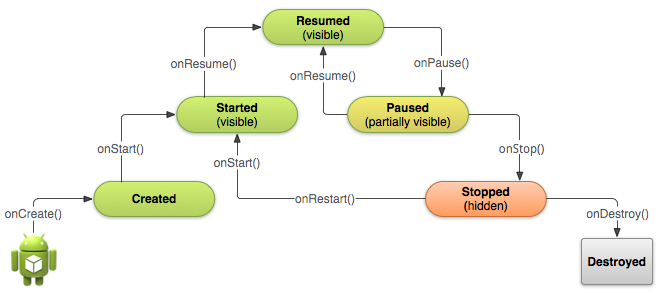
\includegraphics[width=\textwidth]{Images/Android/basic-lifecycle.png}
  \caption[Activity lifecycle]{Simplified scheme of the Activity lifecycle. Source: https://developer.android.com/training/basics/activity-lifecycle/starting.html\#lifecycle-states}
  \label{fig:act_lifec}
\end{figure}

\subsubsection{Fragment Lifecycle}
The lifecycle of a Fragment is closely related to the lifecycle of the Activity that contains it: for example, when an Activity is paused, all the contained Fragments are paused too. In addition to this, however, Fragments can go through lifecycle changes independently of their host Activity: in particular, since Fragments can be dynamically added and removed at runtime, they can be created and destroyed while the Activity is running. Moreover, the developer also has the option to store removed fragments in the so-called backstack and be able to restore them later for example when the user presses the "back" button.\medskip \\
Like Activities, Fragments are characterized by three static states:
\begin{itemize}
	\item Resumed: the Fragment is visible and can receive user input.
	\item Paused: the Activity that contains this Fragment is \textit{partially} hidden by another visual component and has lost the focus.
	\item Stopped: the Fragment is completely hidden to the user. This can happen if the host Activity is also not visible (i.e. in background) or if the Fragment has been stored in the backstack. Like Activities, stopped Fragments are still "alive" and their state is retained.
\end{itemize}
Lifecycle management for Fragments is very similar to the one for Activities, since all callbacks are the same. Fragments provide, however, additional methods to manage the interaction with the host Activity: for example \texttt{onAttach()} is called when the Fragment is linked to an Activity, \texttt{onCreateView()} when the Fragment is ready to build its UI, etc. Figure \ref{fig:fra_lifec} shows the main Fragment callbacks.\bigskip \\
Another characteristic of Fragments is that their instance can be retained, if the developer chooses to do so. This means that the Fragment instance is kept even if the Activity is recreated (e.g. the device screen is rotated), allowing to skip time-consuming initializations.
\begin{figure}
  \centering
  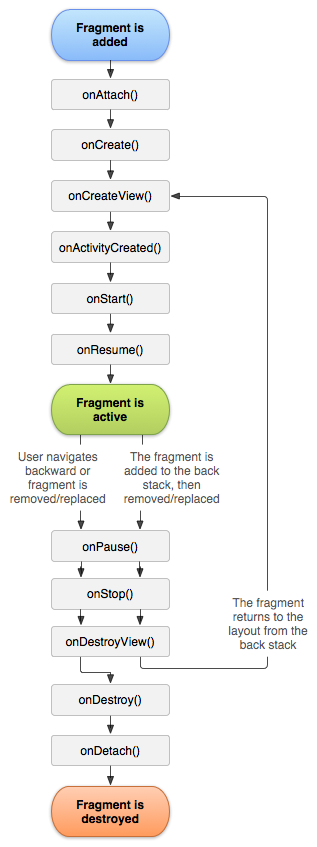
\includegraphics[width=180px]{Images/Android/fragment_lifecycle.png}
  \caption[Fragment lifecycle]{Main fragment lifecycle callbacks. Source: https://developer.android.com/guide/components/fragments.html\#Creating}
  \label{fig:fra_lifec}
\end{figure}

\subsubsection{Managing the Lifecycle}\label{managing_lifecycle}
Handling the components lifecycle is a critical aspect in developing an Android application and it is often source of bugs or unexpected behaviors. For example, properly implementing Activity/Fragment lifecycle methods ensures that the app:
\begin{itemize}
	\item Does not waste system resources (e.g. device sensors) while the user is not interacting with it.
	\item Stops its execution when the user leaves the application (for example a game should pause if the user receives a phone call).
	\item Retains its state if the user leaves and then returns to the application (e.g. a messaging app must keep a partially written message even if the user puts the app in background for a moment).
	\item Does not crash or loses user progress when lifecycle changes occur (e.g. an app that does not correctly manage lifecycle may crash with a NullPointerException if an internal component was destroyed during \texttt{onStop()} but not restored during \texttt{onStart()}).
	\item Adapts to configuration changes (like a device rotation between landscape and portrait modes) without losing data or crashing.
\end{itemize}\medskip
In general, for Activities and Fragments the developer should make sure to:
\begin{itemize}
	\item During \texttt{onCreate()}:
	\begin{itemize}
		\item Set the layout resource defining the UI.
		\item Initialize View components (e.g. add click listeners to buttons).
		\item Initialize the component logic (e.g. class-scope variables).
		\item Restore the previous state (if any) saved during \texttt{onSaveInstanceState()} [this can be alternatively performed during \texttt{onRestoreInstanceState()}].
	\end{itemize}
	\item During \texttt{onRestart()}:
	\begin{itemize}
		\item Requery raw Cursor objects previously deactivated during \texttt{onStop()}.
	\end{itemize}
		\item During \texttt{onStart()}:
	\begin{itemize}
		\item Acquire "secondary" resources (e.g. Broadcast Receiver).
		\item Verify system features (e.g. GPS enabled), because they may change when the application is in background.
	\end{itemize}
	\item During \texttt{onResume()}:
	\begin{itemize}
		\item Start animations and similar CPU-intensive operations.
		\item Acquire "critical" resources (e.g. camera, sensors).
		\item Should \textit{not} restart on-going operations that require user visibility (e.g. games, videos), but let the user decide when to do so.
	\end{itemize}
	\item During \texttt{onPause()}:
	\begin{itemize}
		\item Commit unsaved changes made by the user (e.g. save a draft for an unfinished email), if it does not require too much time.
		\item Stop animations and other operations that may be consuming CPU.
		\item Stop on-going operations that require user visibility (e.g. games, videos).
		\item Release "critical" resources (e.g. camera, sensors).
		\item Should \textit{not} perform any long running operation, the time complexity of this method should be as low as possible.
	\end{itemize}
	\item During \texttt{onStop()}:
	\begin{itemize}
		\item Release "secondary" resources (e.g. Broadcast Receiver).
		\item Perform CPU-intensive shutdown operations (e.g. write unsaved data to database).
	\end{itemize}
	\item During \texttt{onDestroy()}:
	\begin{itemize}
		\item Stop background threads created during \texttt{onCreate()}.
		\item Release long-running resources that could create memory leaks.
		\item Should \textit{not} save data, because the method may not be called in all situations.
	\end{itemize}

\end{itemize}

\section{Event-based Systems}

\subsection{Event-Driven Architecture}
Event-Driven Architecture is a software pattern where the focus is on generation and reaction to events. An event can be defined as a message generated by a producer that represents a change of state or a relevant action performed by a component/actor (e.g. the user). Once generated, events are sent via event channels to all the consumers that are interested to them. Event-Driven Architectures are:
\begin{itemize}
	\item Extremely loosely coupled: the producer does not know about the consequences of its events. It just generates them and then it's up to the consumers to manage everything else.
	\item Well distributed: an event can be anything and exist almost anywhere.
\end{itemize}

\subsection{Android as an Event-Driven Architecture}
Android is implemented as an event-based system. This is because a mobile device must manage several events, like clicks on the touchscreen, sensor data, network requests/responses, etc.\bigskip \\
From an application point of view, events can be generated internally (e.g. from a service/thread created by the application itself) or externally (e.g. sensor data). Each application is composed of several threads, a subset of which, called Looper threads, are in charge of processing events by invoking an appropriate event Handler for each of them.\medskip \\
Events from a single thread are atomic, i.e. they are placed in a FIFO event queue and processes one by one. However, events produced by several threads are processed concurrently and not guaranteed to be ordered or atomic. For example the user may click on a button while the application receives a network response and the device broadcasts some sensor data.\medskip \\
\begin{figure}
  \centering
  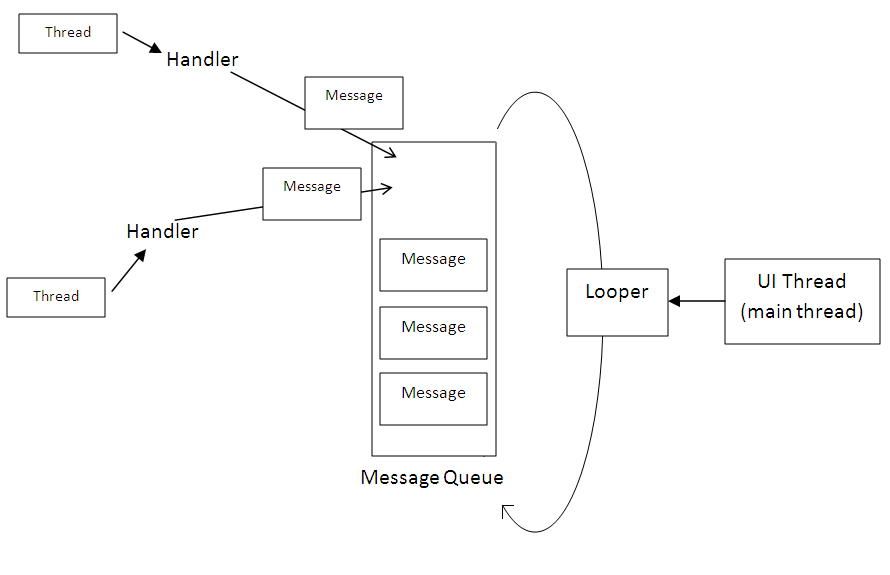
\includegraphics[width=300px]{Images/Android/event-driven.png}
  \caption[Android event handling]{Simplified scheme of Android event handling. Source: https://guides.codepath.com/android/Repeating-Periodic-Tasks}
\end{figure}\\
Examples of events that can be observed in an Android application are:
\begin{itemize}
	\item User input events can be observed attaching listeners to View components. An event listener is a Java interface whose methods are called by the Android framework when the View is triggered by user interaction, for example the \texttt{onClick()} callback of a listener attached to a Button will be called when the user clicks on that button. The developer can then implement the callback to perform any action in response to the input event generation, e.g. starting another activity.
	\item Lifecycle events are triggered when there is a state transition of some component, like an Activity. For example the \texttt{onPause()} callback is invoked when an Activity is paused.
	\item Broadcast events like system messages (e.g. device boot completed, alarm goes off, etc.) or application-specific messages are received by Broadcast Receivers in the \texttt{onReceive()} callback.
	\item Asynchronous messages from services external to the application (e.g. sensor data, network requests, etc.) also have their specific callbacks.
\end{itemize}

\subsection{Event Concurrency Errors}
The concurrency among events inside a single application can lead to unexpected behaviors or crashes.\medskip \\
When the Android developer decides to explicitly create a multi-threaded application we may have the classical problems of concurrency like synchronization, deadlocks and starvation, but problems arise even if he/she does not manually create threads, due to the aforementioned concurrency of events.\medskip \\
In this context, the most relevant challenge in an Android application is race conditions: two or more events do not happen in the order the programmer intended. As an example, reported in listing~\ref{lst_event_race_first}, a race condition may happen when the developer starts an AsyncTask (an utility class that allows to perform short operations in the background without blocking the UI thread) to asynchronously perform some operation. If the user, for example, rotates the device while the AsyncTask is running, the application crashes with an \texttt{IllegalStateException} because the reference to the old view is lost.


%..............................................................................%
%............................ STATE OF THE ART ................................%
%..............................................................................%


\newpage
\part{Android Testing State of the Art}\label{part_state_art}

Android test cases adhere to the JUnit~\cite{JUnit} format, a testing framework for Java. It allows to create classes called test cases that contain methods annotated with \texttt{@Test}, each representing a test.

\section{Unit Testing}
White-box unit testing in Android can be:
\begin{itemize}
	\item Local: it runs on the local development machine (i.e. the computer where the application is coded). It has the advantage of being fast (avoids the overhead to load the application in a device/emulator), but can be exploited only if the tested unit has no dependencies or simple dependencies. This means that the test case should not use any device-specific features (e.g. expect a sensor input) or, if it does so, they should be minimal since they need to be mocked using for example tools like Mockito~\cite{Mockito}.
	\item Instrumented: it is executed on a physical device or on an emulator and so has access to the full instrumentation environment. It is slower than the previous case but it's more convenient if the unit dependencies are too complex to mock.
	\item Hybrid: the external library Robolectric~\cite{Robolectric} tries to take the advantages of the two previous approaches, i.e. it runs "instrumented" tests on the local machine, without mocking. As reported on the website, Robolectric allows a test style that is closer to black box testing, making the tests more effective for refactoring and allowing them to focus on the behavior of the application instead of the implementation of Android.
\end{itemize}
\begin{figure}
  \centering
  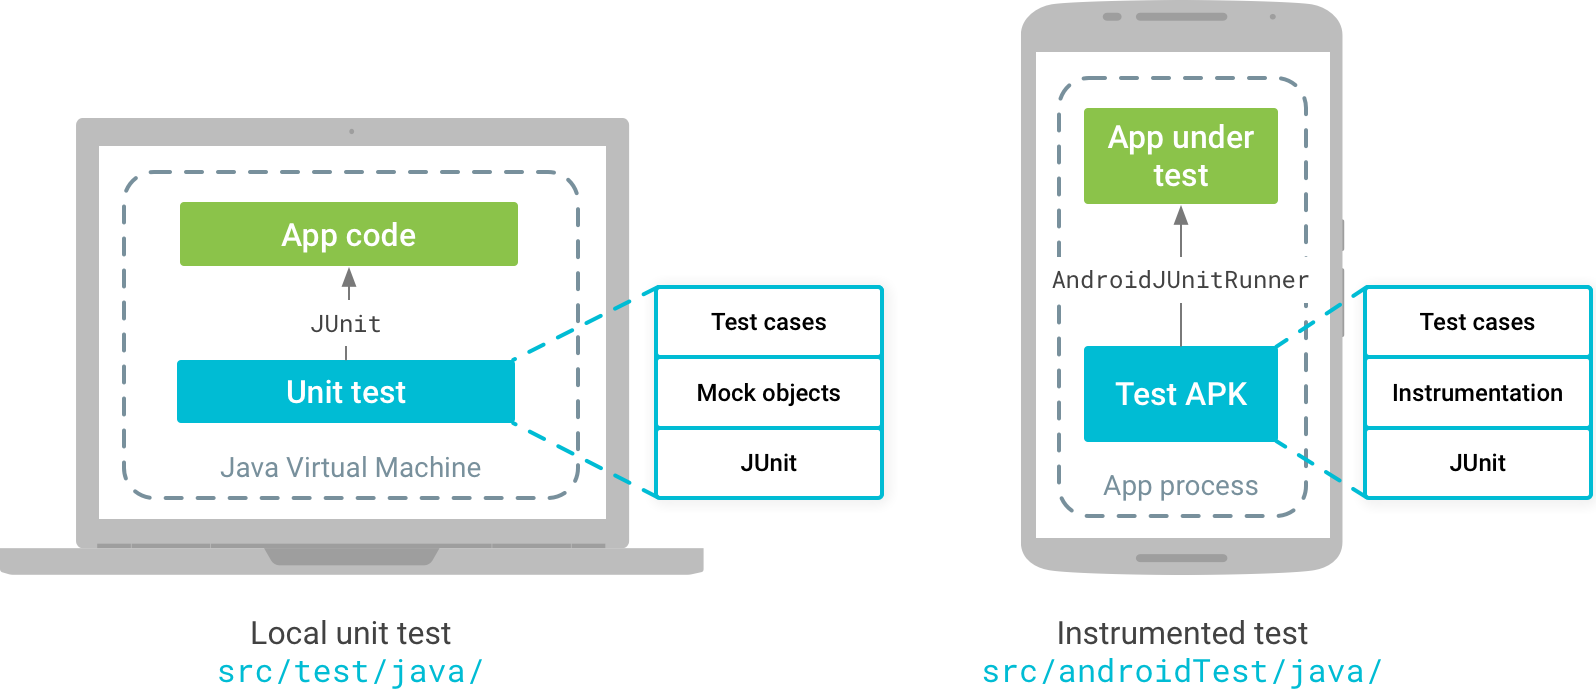
\includegraphics[width=250px]{Images/Android/test-types.png}
  \caption[Local and instrumented Android tests]{Local and instrumented Android tests. Source: https://developer.android.com/training/testing/start/index.html\#test-types}
\end{figure}

\section{UI Testing}
Android also provides a way to test User Interface (UI) to see if it behaves as expected. This type of testing can be defined as a grey-box approach: the application is tested at the user level without considering the actual implementation of the UI, but the definition of the test cases may require to know some information on the internal structure, for example the IDs of the buttons to be clicked.\medskip \\
We may have:
\begin{itemize}
	\item UI testing on a single app: the Espresso~\cite{Espresso} library provides APIs for writing UI tests to simulate user interactions. In general, defining a test case means building a series of \texttt{onView(Matcher).perform(ViewAction).check(ViewAssertion)} instructions, i.e. select a particular View that matches a description (e.g. a button with "Start" text), perform one or more actions on it (e.g. click) and check if some conditions are true (e.g. if after the click the button text changes). The main advantages of Espresso are that the test cases are easily readable and understood, and that it has automatic synchronization (before performing an action it waits for the previous ones to be completed, i.e. for the main thread to be idle).
	\item UI testing on multiple apps: the UI Automator~\cite{UIAutomator} library allows to test if the developed application interacts correctly with the system or other apps (e.g. the application may request an image, the Camera app is opened, the picture is taken and then the control goes back to the original application). 
\end{itemize}

\section{Runner Tools}
In addition to the testing frameworks described in the previous sections, Android also offers some tools to run and test an application without accessing the source code (black-box testing):
\begin{itemize}
	\item UI Exerciser Monkey~\cite{UIExerciserMonkey}: allows to run an application on a physical device or emulator generating a repeatable pseudo-random stream of user events (e.g. clicks) and system-level events (e.g. start call). The developer can set several options like target package, probability of certain events, etc.
	\item monkeyrunner~\cite{monkeyrunner}: controls a device or emulator from a workstation by sending specific commands and events defined as a Python program. It also allows to take screenshots during the test execution and store them on the workstation.
\end{itemize}

\section{Lifecycle Testing}
Due to the importance of lifecycle handling, some approaches to test applications focusing on this aspect have been developed.

\subsection{Testing Frameworks Support}
The built-in instrumented testing framework allows to drive an Activity lifecycle via the methods \texttt{callActivityOnStart()}, \texttt{callActivityOnPause()}, etc. provided by the \texttt{Instrumentation} class. These methods, however, are complex to use because the developer needs to chain the correct methods in each test case to simulate a valid lifecycle transition (e.g. for example to simulate the Activity being closed the developer needs to call in order pause, stop and destroy) and, since they are required to run on the main thread of the application, often need to be executed inside a \texttt{Runnable} that may require explicit synchronization with the testing thread.\bigskip \\
The Robolectric framework makes things a little easier allowing the developer to specify a chain of transitions like \texttt{buildActivity(MyActivity.class).create().start().resume()}, avoiding \texttt{Runnable} and synchronization problems. This approach, however, suffers the same problem of the instrumented framework: it requires explicit calls to the correct chain of transitions to simulate realistic behaviors, and so coded by the developers only in very specific situations.

\subsection{THOR}
One example of tool designed with particular regard to lifecycle handling is THOR~\cite{Adamsen:2015:SEA:2771783.2771786}. The idea of the tool is to run pre-existing UI test cases (defined in Robotium or Espresso) in adverse conditions to test the application robustness. These adverse conditions are not, however, unusual events, but common expected behaviors of the application: in particular, THOR injects in the tests several neutral system events, i.e. events that are not expected to change the outcome of the test. These neutral events are mainly related to Activity lifecycle: for example Pause $\rightarrow$ Resume; Pause $\rightarrow$ Stop $\rightarrow$ Restart; Audio
focus loss $\rightarrow$ Audio focus gain. Neutral events injected in an application that does not manage the lifecycle correctly can lead to the discovery of bugs, which are not necessarily crashes but also unexpected behaviors for the specific application.\medskip \\
The tool provides several features like:
\begin{itemize}
	\item Neutral events are injected in suitable locations to avoid conflicts with the test case: in particular they are triggered when the event queue becomes empty and the execution of the remaining test is delayed.
	\item Multiple errors for each test: if a test fails after some neutral event injections, the test is rerun but injections are only performed after the previous failure point to maximize error detection.
	\item Faults Localization: if a test fails, the tool tries to identify the exact causes (i.e. the neutral events responsible for the unexpected behavior) using a variant of delta debugging (scientific approach of hypothesis-trial-result loop), then displays this information to the user to allow further investigation.
	\item Faults Classification: the errors that make the test cases fail are classified by importance and criticality.
	\item Customization: the developer can select the set of tests to run,
the set of neutral event sequences to take into account, and
several other different variations.
\end{itemize}
While very effective and useful for bug detection, THOR is not a user-friendly tool. First of all the tests are executed via an external program (and so the developer is not able to simply run the tests via an IDE like Android Studio), that is only available for Linux and its installation is not immediate. Moreover, THOR only executes the test cases on an emulator running Android KitKat 4.4.3, which does not leave any choice to the developer on which version of Android to test. In addition to this, the pre-defined test cases on which the tool works need to be well structured: if they do not reach a faulty portion of the application, the neutral events never allow the bug detection.

\section{Race Conditions Testing}\label{section_race_tools}
Due to the relevance of the race conditions problem, several research studies tried to provide a way to detect them.

\subsection{CAFA}
For example, CAFA~\cite{Hsiao:2014:RDE:2666356.2594330} is a tool that allows to detect use-free races. The authors note that thousands of events may get executed every second in a mobile system and that, even if they are processed sequentially in one thread, most of them are logically concurrent. These concurrent events could be commutative with respect to each other, i.e. the result is the same even if they are executed in a different order. The tool determines if two events are commutative or not, restricting the focus on use-after-free violations (a reference is used after it has been freed, i.e. it does not point to an object anymore). If two events where one uses and the other frees a reference are logically concurrent, they must be non-commutative. To detect possible racy behaviors, the tool analyzes the traces of the low-level read and write operations, as well as certain branch instructions. While CAFA is a good starting point for race condition analysis, its main problems are that it's fairly slow (it may take hours to analyze an application), only focuses on a very specific type of race conditions and the tool is not publicly available.

\subsection{EventRacer}
Android EventRacer~\cite{Bielik:2015:SRD:2858965.2814303} is an improvement of CAFA, defined by the authors as the first scalable analysis system for finding harmful data races in real-world Android applications. EventRacer not only analyzes use-free races, but also other types of race conditions like:
\begin{itemize}
	\item Data Races Caused by Object Reuse: list components in Android, like ListView, usually reuse rows while the user scrolls, to improve performance (i.e. avoid instantiating as many rows as the number of data values). If the content of each row is loaded asynchronously, it may happen that the wrong data is loaded in a row (the user scrolled the list in the meanwhile and the row has already been reused).
	\item Data Races Caused by Invalidation: these are the races similar to the first example in listing \ref{lst_event_race_first}, i.e. the AsyncTask completing when the Activity has already been rotated.
	\item Callback Races: different listener callbacks may be invoked in any order. For example the developer may asynchronously create a GoogleMap object and request location updates from the device GPS. They may expect the \texttt{onMapReady()} callback to be executed before the first \texttt{onLocationChanged()} callback (and so use the map to place a marker at the received location), but it might not be the case.
\end{itemize}
Moreover, EventRacer analyzes an application in much less time than CAFA: building the Happens-Before relationship graph has $\mathcal{O}(n^2)$ time complexity instead of $\mathcal{O}(n^3)$. The tool is also publicly available as an online tester or an offline application (only available for Linux systems). One disadvantage of the EventRacer approach is that the implementation requires to modify the Android framework in order to access low-level information and, for this reason, it is only available for Android 4.4, which limits the options of the developer for testing other versions of the OS. Another critical aspect of the tool is that detection is performed by running the application in an emulator feeding it with pseudo-random events: this approach may skip several sections of an application, especially if they are not immediately available (e.g. they require user sign-in).

\fxnote*{New}{\subsection{ERVA}}
The tool ERVA~\cite{Hu:2016:AVR:2931037.2931069} is a further step forward in event race detection. The authors note that the previous tools have several drawbacks like:
\begin{itemize}
	\item They are prone to false positives, due to:
	\begin{itemize}
		\item Imprecise Android Component Model: for example, EventRacer may recognize the callbacks \texttt{onCreateView()} and \texttt{onResume()} as racy, but the Android lifecycle documentation states that they are always called in that order.
		\item Implicit Happens-before Relation: two Runnable objects, if posted to the same Handler, are executed in a FIFO order, but EventRacer may wrongly assume that they can be concurrent.
	\end{itemize}
	\item They cannot verify if it a benign or harmful race. A benign race can be:
	\begin{itemize}
		\item Control Flow Protection: if the access to a variable is protected by an \texttt{if} statement that first checks whether it is null, even if a race occurs there is no impact on the execution.
		\item No State Difference: if the program does not depend on the execution order (e.g. a counter is decreased in the same way by several tasks) a race is meaningless.
	\end{itemize}
	\item They do not give developers a way to reproduce the race.
\end{itemize}
ERVA addresses these issues by splitting the analysis in two phases:
\begin{itemize}
	\item Race detection: the tool runs EventRacer itself to collect all the detected races, recording in the meanwhile replay and synchronization information. With the recorded data, ERVA determines if the race is a false positive.
	\item Race verification: the tool tries to verify if the detected true positives are benign or harmful races. To do so, it exploits the replay data to reproduce the execution by changing the order of some events: if the flipping has no side effect, then the race is benign.
\end{itemize}

\subsection{DEvA}
A completely different approach for race detection is provided by DEvA~\cite{Safi:2015:DEA:2786805.2786836}. The idea of the tool is to base its search on static code analysis rather than dynamic analysis: this approach guarantees more code coverage and completeness. DEvA focuses on a specific type of problem called Event Anomalies: processing of two or more events results in accesses to the same memory location and at least one of those is a write access (note that the use-free races analyzed by CAFA are a subclass of this type of issue). The idea of the tool is to identify variables that may be modified as a result of receiving an event (i.e. a potential Event Anomaly) using the Control Flow Graph of the application (i.e. all paths that may be traversed in the application during its execution). The tool receives as input from the developer:
\begin{itemize}
	\item The list of all methods used as event handlers (callbacks that use the events).
	\item The base class used to implement events in the system.
	\item The set of methods used as consumed event revealing statements (i.e. methods that retrieve information stored in an event without modifying the event's attributes), used to tell apart events when a general parameter is passed to a callback.
\end{itemize}
DEvA allows a very fast analysis (usually 1 or 2 minutes) and guarantees complete code coverage, but static analysis may report false positives or be unable to detect some anomalies.

                                                                                                                                 
\fix{You can conclude the section with a couple of sentences stating that present work addresses the limitations of the state of the art and introduces new X, Y, Z for A, B, C }

%..............................................................................%
%.................................. LIFECYCLE .................................%
%..............................................................................%

\newpage
\part{Lifecycle Testing}\label{part_lifecycle}

\section{Introduction}
Correctly handling a component lifecycle is a key aspect of Android application development, to avoid waste of resources, crashes and unexpected behaviors.\medskip \\
However, the available means to thoroughly test an Activity lifecycle are lacking. The Android testing frameworks provide low-level methods to drive the lifecycle but they need to be carefully chained to simulate realistic behaviors, and existing testing tools like THOR, while effective, present some limitations such as usability issues.\medskip \\
Given this context, the solution proposed by the first part of this thesis provides a more complete support to test a component lifecycle. In particular, two approaches for lifecycle testing are proposed: static analysis and dynamic analysis. The former analyzes the source code of the application to detect possible issues related to the handling of some components in accordance to the host Activity/Fragment lifecycle, for example failing to release a resource that was previously acquired. The dynamic approach, instead, provides to the developer a testing framework to easily drive the lifecycle, with pre-generated test cases for the most common transitions.\medskip \\
The following sections present first the static approach and then the dynamic testing framework.

\section{Static Analysis}\label{section_lifecycle_static}

\subsection{Introduction}
This section presents static lifecycle checks more in detail. First a short introduction of the main concepts of static program analysis is presented, then a detailed explanation of its application in lifecycle testing.

\subsection{Static Program Analysis}
As opposed to dynamic analysis that requires to actually run an application, static analysis only inspects the source code. Static program analysis is mainly employed to highlight possible coding errors (e.g. access a variable that is always null), to formally prove properties (e.g. pre- and post-conditions of a function) and to assess if the software follows a set of coding guidelines (e.g. variable naming conventions). There are several different analysis techniques, here we focus on those that employ the Abstract Syntax Tree and the Control Flow Graph of the problem.\medskip \\
An Abstract Syntax Tree (AST) is a tree representation of the code structure, where each node represents a program construct (e.g. a variable or an instruction). AST Traversal is the static analysis technique that explores the Abstract Syntax Tree to detect possible structural and syntactical problems, such as coding conventions conformity.\medskip \\
A Control Flow Graph (CFG) instead represents the sequence of operations executed along all paths that may be traversed during the execution of the program. Control Flow Analysis employs the CFG to detect possible issues related to the program flow, e.g. accessing a variable that may not have been initialized in all previous paths. Data Flow Analysis is a similar technique that gathers information about the possible set of values in several points of the CFG.

\subsection{Static Lifecycle Checks}
This part of the thesis focuses on possible lifecycle checks using a static analysis approach. The idea is to consider some components used in the applications that require special attention, either because of their own lifecycle or because they need to be carefully used in accordance to the host component lifecycle.\medskip \\
Failing to correctly handle an Activity/Fragment lifecycle may lead to unexpected behaviors or resource waste. An unexpected behavior can be for example the loss of user data: if the developer does not react correctly to an Activity being destroyed in a note-taking app the currently written text may be lost. An example of resource waste can be requesting GPS location updates at constant intervals in an application that uses maps and failing to cancel them when the application is paused/stopped: the system will continue querying the device sensors even if the user is not currently looking at the map.\medskip \\
Static program analysis can help detecting this type of problems. For example, if a method call to acquire a certain component is detected but no call to release it is found in the code, then a warning can be shown to the developer.

\subsection{Target Components}
In this section a more detailed explanation of the target components that are useful to be checked statically is reported.\bigskip \\
Each component is analyzed in terms of:
\begin{itemize}
	\item Release: should the component be always released after it is acquired? If so, the static analysis can check if the call to release is always performed.
	\item Best Practices: in which states of the host Activity/Fragment lifecycle is recommended/usual to acquire and release the component? If there are best practices, the analysis can check if the calls follow them.
	\item Double Instantiation: can acquiring the same component more than once cause unexpected behaviors or waste computational power? If so, the static analysis can check if the resource may be acquired multiple times during the execution.
\end{itemize}
These three aspects were chosen because of their relevance in Android applications and because they are particularly suitable for static analysis, being usually characterized by regular and often strict usage patterns.\bigskip \\
Among the many components that can be used in Android applications, some were chosen and listed below as examples of targets for static lifecycle analysis. These components were selected for their standardization with regard to initialization and destruction: in most situations, the pattern for acquiring and releasing the linked resource is regular, and static analysis can easily assess the conformity with best practices.\bigskip \\
The selected components for static lifecycle analysis are:
\begin{itemize}
	\item Broadcast Receiver: it allows to receive messages from the system or another application component.
	\begin{itemize}
		\item Release: the official documentation states that a Broadcast Receiver, if registered with an Activity context (as it is usually the case), should ideally be unregistered before the Activity is done being destroyed, but if it not so the system will clean up the leaked registration anyway and only log an error. In case the receiver is registered using the Application context, however, it will be never unregistered by the system, so missing a call to the unregister method may lead to significant leaks\footnote{https://developer.android.com/reference/android/content/Context.html\#getApplicationContext()}. Moreover, it is reported that the developer should not unregister during an Activity \texttt{onSaveInstanceState()} method, because it won't be called if the user moves back in the history stack\footnote{https://developer.android.com/reference/android/content/BroadcastReceiver.html}.
		\item Best Practices: the only official recommendation on how to handle a Broadcast Receiver in accordance to the lifecycle of the Activity/Fragment that uses it is to unregister it during \texttt{onPause()} if it is registered during \texttt{onResume()}\footnote{https://developer.android.com/reference/android/content/BroadcastReceiver.html}. The common usage of the receiver is to register during \texttt{onResume()} or \texttt{onStart()} and to unregister during \texttt{onPause()} or \texttt{onStop()} respectively.
		\item Double Instantiation: registering twice a Broadcast Receiver with the same parameters does not create any correctness issue and the complexity of the method is negligible, so there's no need to check double instantiation for this component. However, if the Broadcast Receiver is unregistered twice the system throws an \texttt{IllegalArgumentException}, so it might be useful to warn the developer in advance if two calls are detected.
	\end{itemize}
	\item Google API Client: the \texttt{GoogleApiClient} class allows to connect to the Google Play services for several APIs, like Google+, Google Drive, wearables, etc. The developer can either manage the connection manually or leave it to the system. The following specifications are of course valid for the former case.
	\begin{itemize}
		\item Release: the API Client should always be disconnected when the application is done using it. This fact is not clearly stated in the documentation, but, given the best practices described in the next element, it is safe to assume that it is required.
		\item Best Practices: the official recommendation is to connect during \texttt{onStart()} and to disconnect during \texttt{onStop()}\footnote{https://developers.google.com/android/guides/api-client\#start\_a\_manually\_managed\_connection}. \fix{use package \texttt{url} and wrap the references in it, should simplify your life}
		\item Double Instantiation: it is not a problem since the call to \texttt{connect()} returns immediately if the client is already connected or connecting\footnote{https://developers.google.com/android/reference/com/google/android/gms/common/api/GoogleApiClient\#public-methods}.
	\end{itemize}
	\item Fused Location Provider API: the \texttt{FusedLocationProviderApi} class allows to query information about the current location. In particular, we are interested in the functionality that allows to receive periodic updates.
	\begin{itemize}
		\item Release: the location updates should be removed by calling the \texttt{removeLocationUpdates()} method.
		\item Best Practices: the official documentation encourages the developer to think whether it may be useful to stop the location updates when the Activity is no longer in focus, to reduce power consumption while the app is in background\footnote{https://developer.android.com/training/location/receive-location-updates.html\#stop-updates}.
		\item Double Instantiation: does not need to be considered since any previous location updates are replaced by the call to \texttt{requestLocationUpdates()}\footnote{https://developers.google.com/android/reference/com/google/android/gms/location/FusedLocationProviderApi\#public-methods}.
	\end{itemize}
	\item Camera:
		\begin{itemize}
			\item \texttt{Camera} class: this is the older API to control the device camera, deprecated in API level 21 (Lollipop).
			\begin{itemize}
				\item Release: releasing the camera is fundamental. Failing to do so means that all the applications on the device will be unable to use it\footnote{https://developer.android.com/reference/android/hardware/Camera.html\#release()}.
				\item Best Practices: the best practice is to acquire the camera during \texttt{onResume()} and release it during \texttt{onPause()}\footnote{https://developer.android.com/reference/android/hardware/Camera.html}.
				\item Double Instantiation: if the developer tries to acquire the camera twice, the system will throw a runtime exception\footnote{https://developer.android.com/reference/android/hardware/Camera.html\#open(int)}.
			\end{itemize}
			\item \texttt{camera2} package: this is the new API introduced in Android Lollipop to manage the device camera
			\begin{itemize}
				\item Release: although the documentation does not clearly state that the developer \textit{must} release the components, the objects used to manage the camera such as \texttt{ImageReader}\footnote{https://developer.android.com/reference/android/media/ImageReader.html\#close()}, \texttt{CameraDevice}\footnote{https://developer.android.com/reference/android/hardware/camera2/CameraDevice.html\#close()}, \texttt{CameraCaptureSession}\footnote{https://developer.android.com/reference/android/hardware/camera2/CameraCaptureSession.html\#close()}, etc. all provide a \texttt{close()} method to release the resource. In the sample application provided by Google\footnote{https://github.com/googlesamples/android-Camera2Basic/blob/master/Application/src/main/java/com/example/android/camera2basic/Camera2BasicFragment.java} these methods are all called during \texttt{onPause()} and a \texttt{Semaphore} is used "to prevent the app from exiting before closing the camera", so it is safe to assume that releasing these resources is required.
				\item Double Instantiation: methods to acquire the components like \texttt{setRepeatingRequest()}\footnote{https://developer.android.com/reference/android/hardware/camera2/CameraCaptureSession.html\#setRepeatingRequest(android.hardware.camera2.CaptureRequest, android.hardware.camera2.CameraCaptureSession.CaptureCallback, android.os.Handler)}, \texttt{createCaptureSession()}\footnote{https://developer.android.com/reference/android/hardware/camera2/CameraDevice.html\#createCaptureSession(java.util.List<Candroid.view.Surface>, android.hardware.camera2.CameraCaptureSession.StateCallback, android.os.Handler)}, etc. replace the previous calls. For this reason, there's no need to check double instantiation for correctness, but since the time complexity of most of these calls is significant (e.g. \texttt{createCaptureSession()} "can take several hundred milliseconds") it can be checked for performance reasons.
			\end{itemize}
		\end{itemize}
	\item Ads View: the \texttt{AdView} class is a View used to display banner advertisements.
	\begin{itemize}
		\item Best Practices: the class provides methods like \texttt{destroy()}, \texttt{pause()}, etc. that should be called in the Activity/Fragment lifecycle methods with similar name (\texttt{onDestroy()}, \texttt{onPause()}, etc.)\footnote{https://developers.google.com/android/reference/com/google/android/gms/ads/AdView}.
	\end{itemize}
\end{itemize}\medskip
Other components, such as Services or Threads, should also be carefully managed according to the lifecycle. They are not listed above because, since there are too many different use cases (e.g. a Service may be active during several Activities, work when the application is in background, etc.), it is difficult to extract a list of best practices and, as a consequence, to statically check the code for misuse.

\subsection{Design}
Given the chosen target components, the static analysis tool can help the developer detecting the outlined issues and best practices. In particular, the thesis focuses on two significant examples:
\begin{itemize}
	\item Broadcast Receiver: to implement the static check, the tool only focuses on single Java classes. Even though it is possible to use the same receiver across multiple classes (e.g. passing the reference as a method parameter), it is not a common approach, and so the running complexity may be decreased without loss of much detection power.
	\begin{itemize}
		\item Release: the static tool detects registrations and unregistrations in the class and, if a pair is not found, shows a warning. The detection is performed considering the name of the variable of the considered Broadcast Receiver: even if it is possible to have two different variables referencing the same receiver, it is not common and so we can avoid performing a complex Control Flow Analysis, and employ an AST Traversal technique instead. This check is performed for all registrations, both with Activity and Application Context, since even in the former case it is better to unregister to avoid possible overheads in the automatic system clean-up.
		\item Best Practices: the tool checks if the call to unregister is performed inside the \texttt{onSaveInstanceState()} method of a Fragment or an Activity and, if so, shows a warning to the developer. This is performed by AST Traversal to check in which class and method the unregistration is performed.
		\item Double Instantiation: the tool detects multiple unregistrations of the same receiver inside the class and, in that case, shows a warning. Only the unregistrations outside a try/catch block are considered, since if the developer catches the IllegalStateException that may be generated it is possible to have multiple unregistrations.
	\end{itemize}
	\item Google API Client: the analysis is similar to the Broadcast Receiver case. The tool focuses on single Java classes, since it's unusual to connect in one class and disconnect in another.
	\begin{itemize}
		\item Release: if a call to the connection method is detected but a disconnection is not, the tool shows a warning. Detection is performed via AST Traversal because, given the strict best practice to use \texttt{onStart()} and \texttt{onStop()}, it is not worth to use a Control Flow Analysis to actually see if the disconnection is called in every path following the connection.
		\item Best Practices: if via AST Traversal the tool detects that the current class is an Activity or a Fragment, it shows a warning if connection and disconnection are not performed in \texttt{onStart()} and \texttt{onStop()} respectively.
	\end{itemize}
\end{itemize}

\subsection{Implementation}

\subsubsection{Introduction}
For the implementation of the static checks~\cite{RepositoryStatic} Android Lint was chosen, of which a more detailed description is reported in the next section. After this, the actual implementation structure is explained.

\subsubsection{Android Lint}
Android Lint~\cite{Lint} is a static analysis tool that scans Android projects for potential bugs, performance, security, usability, accessibility and internationalization issues, and more. It is an IDE-independent analyzer, at the moment integrated with Eclipse and Android Studio.\medskip \\
Some of the checked issues are run directly when the user is writing the code and shown via an in-line warning. A more complete analysis can be performed by explicitly running the tool on the whole project, via terminal command or directly from the IDE options. The results are then presented in a list with a description message and a severity level, so that the developer can easily identify the most critical problems and understand their causes. It is also possible to customize the checker for example by specifying the minimum severity level of the detected issues and by suppressing some specific checks if the developer is not interested.\medskip \\
Android Lint provides more than 100 built-in checks. Some examples:
\begin{itemize}
	\item MissingPermission (correctness issue): Lint detects that a call to some method (e.g. store a file on the SD card) requires a specific system permission (e.g. access to external storage) that has not been included in the application manifest.
	\item WrongThread (correctness issue): checks that the methods that must run on the UI thread (e.g. manipulation of a View component) are actually called there.
	\item SecureRandom (security issue): detects random numbers generated by fixed seeds, usually employed only during debugging.
	\item UnusedResources (performance issue): a resource like an image, a string, etc. is not used in the application and so it can be deleted to free space.
	\item UselessParent (performance issue): a layout file contains a View component that is of no use and can be removed for a more efficient layout hierarchy.
	\item ButtonOrder (usability issue): makes sure that "cancel" buttons are placed on the left of the UI component, to follow the Android Design Guidelines.
	\item ContentDescription (accessibility issues): checks that important visual elements like image-buttons have a textual description to allow the system accessibility tools to describe their purpose.
	\item HardcodedText (internationalization issue): makes sure that text strings displayed to the user are placed on the appropriate XML files to allow translation and not hard-coded in Java.
\end{itemize}

\subsubsection{Custom Android Lint Checks}
\textit{Important note: the Lint API is not final and mostly undocumented. This means that what is reported below is based only on a few examples/tutorials found on the Internet, on the built-in checks implementations and on source code inspection, and not on official documentation. Moreover, since it is not final, future releases of the tool may invalidate the following statements and the custom implementations.}\bigskip \\
The open source Android Lint API allows to build custom rules for the static analyzer.\medskip \\
Implementing a custom Lint rule means building four components:
\begin{itemize}
	\item Issue: a problem detected by the rule, characterized by properties like ID, explanation, category, priority, etc. For example the "MissingPermission" issue has "9/10" priority, "Error" severity, "Correctness" category and an explanation describing the problem to the developer.
	\item Detector: a detector is in charge of identifying one or more issues (if more than one, they are independent but logically related). For example the built-in \texttt{ButtonDetector} identifies the "Order" (cancel button on the left), "Style" (button borders), "Back" (avoid custom back buttons) and "Case" (capitalization of "OK" and "Cancel" labels on buttons) issues.
	\item Implementation: links an issue to a detector and specifies the rule scope.
	\item Registry: it is simply in charge of registering the issues to allow the Lint tool to identify the custom rules.
\end{itemize}\bigskip
More in detail, a custom detector extends the \texttt{Detector} class and implements one (or more in special cases) of these interfaces:
\begin{itemize}
	\item \texttt{XmlScanner} if it needs to analyze XML files (such as the application manifest or layout descriptions).
	\item \texttt{JavaScanner} if it needs to analyze Java files (source code for classes).
	\item \texttt{ClassScanner} if it needs to analyze Class files (compiled Java files).
\end{itemize}
The extended class and the interfaces provide some utility methods that can be overridden by the developer to filter applicable files (e.g. name contains a given substring), nodes (e.g. only variable declarations), elements (e.g. an XML scanner only wants to read \texttt{TextView} elements), etc. to focus the rule attention only on particular situations and improve performance.\\
In particular, a detector that implements \texttt{JavaScanner} is able to visit the Java files via an Abstract Syntax Tree, represented with the \texttt{lombok.ast} API. The developer has two options:
\begin{itemize}
	\item Use the \texttt{Detector} callback methods to visit the nodes using the default AST Visitor. First of all, if the detector is interested only in specific types of nodes in the AST (as it is usually the case) the developer should override the \texttt{getApplicableNodeTypes()} method and return a list of types (e.g. \texttt{ClassDeclatation}, \texttt{MethodInvocation}, etc.). The class also provides several other methods to focus the search, like \texttt{getApplicableMethods()} (return list of method names), \texttt{applicableSuperClasses()} (return list of super-classes names), etc. Once this is done, the developer can override the detector methods like \texttt{visitMethod()} to receive all matching method invocations found in the tree, \texttt{checkClass()} to receive the matching class declarations, etc. to implement the rule logic.
	\item Return in \texttt{createJavaVisitor()} method a custom implementation of the AST Visitor (subclass of \texttt{AstVisitor}) that implements the rule logic. Inside the AST Visitor the developer can override one or more methods that allow to visit every type of node in the tree such as \texttt{visitMethodDeclaration()}, \texttt{visitVariableDeclaration()}, \texttt{visitAnnotation()}, \texttt{visitWhile()}, etc. 
\end{itemize}
If a problem is found during one of the callbacks, the detector can call the \texttt{report()} method to pass the issue, the location (i.e. file and line) and a message in order to show the warning to the developer.\smallskip \\
Note that some detectors can just visit the nodes and immediately recognize and report an error (e.g. if an attribute of a given component is not set), but others may require to do more expensive computation (even across multiple files). If this is the case, the developer can use the detector's \texttt{afterProject()} hook that is called when the whole project has been analyzed. In order to decide if a problem is present or not, the developer needs to save the state of the computation: variables like boolean flags can be easily stored in the detector object, but the problem is with code locations. Computing the location of an issue is an expensive operation and, especially if the probability of error is very low, we may have performance issues (e.g. a detector that finds unused resources cannot store the location of each of them before finding out that they are actually used somewhere). To solve this issue the developer can store location handles (lightweight representations of locations that can later be fully resolved if the problem is actually present) or request a second pass to the Lint tool (i.e. in the first project analysis one only sets some flags to detect problems, then if that is the case the project is scanned again to gather the actual locations of the issues).\medskip \\
The Android Lint tool also provides the means to perform Control Flow Analysis during the detection process. In particular, the \texttt{ControlFlowGraph} class allows to build a low-level Control Flow Graph containing the \textit{insns} nodes of a method, i.e. the RTL (Register Transfer Language) representation of the code where each \textit{insns} node is a bytecode instruction (e.g. jump). This Control Flow Graph can be useful for example to analyze if some component is always released, e.g. the built-in \texttt{WakelockDetector} uses it to see if, when the Wake-Lock (a lock to keep the device awake) is acquired in a method, it is released afterwards in every possible path.\bigskip \\
Issues are usually defined as public, final and static fields inside their detector class. They are simply objects of the \texttt{Issue} class that are instantiated calling \texttt{Issue.create()} with some parameters like ID, category, severity, etc.\bigskip \\
Implementations are objects of the \texttt{Implementation} class, whose constructor requires the detector class and the scope (e.g. \texttt{Scope.JAVA\_FILE\_SCOPE}). The implementation is passed as the last parameter of the \texttt{Issue.create()} method to link the issue with the detector.\bigskip \\
Finally, registers are sub-classes of \texttt{IssueRegistry} that usually only override the \texttt{getIssues()} method to return the list of custom issues. The registry must be referenced in the \texttt{build.gradle} file (in Android Studio) or in a manifest file (in Eclipse) to allow Lint to find it.\bigskip \\
Once every component has been implemented, to actually include the Lint check in the list of rules enforced by the tool one must copy the generated JAR file of the library in the \texttt{$\sim$/.android/lint/} directory. Using Gradle in Android Studio, one can write a snippet to automatically copy the JAR after each \textit{install} command.

\subsubsection{Code Structure}
\begin{figure}
  \centering
  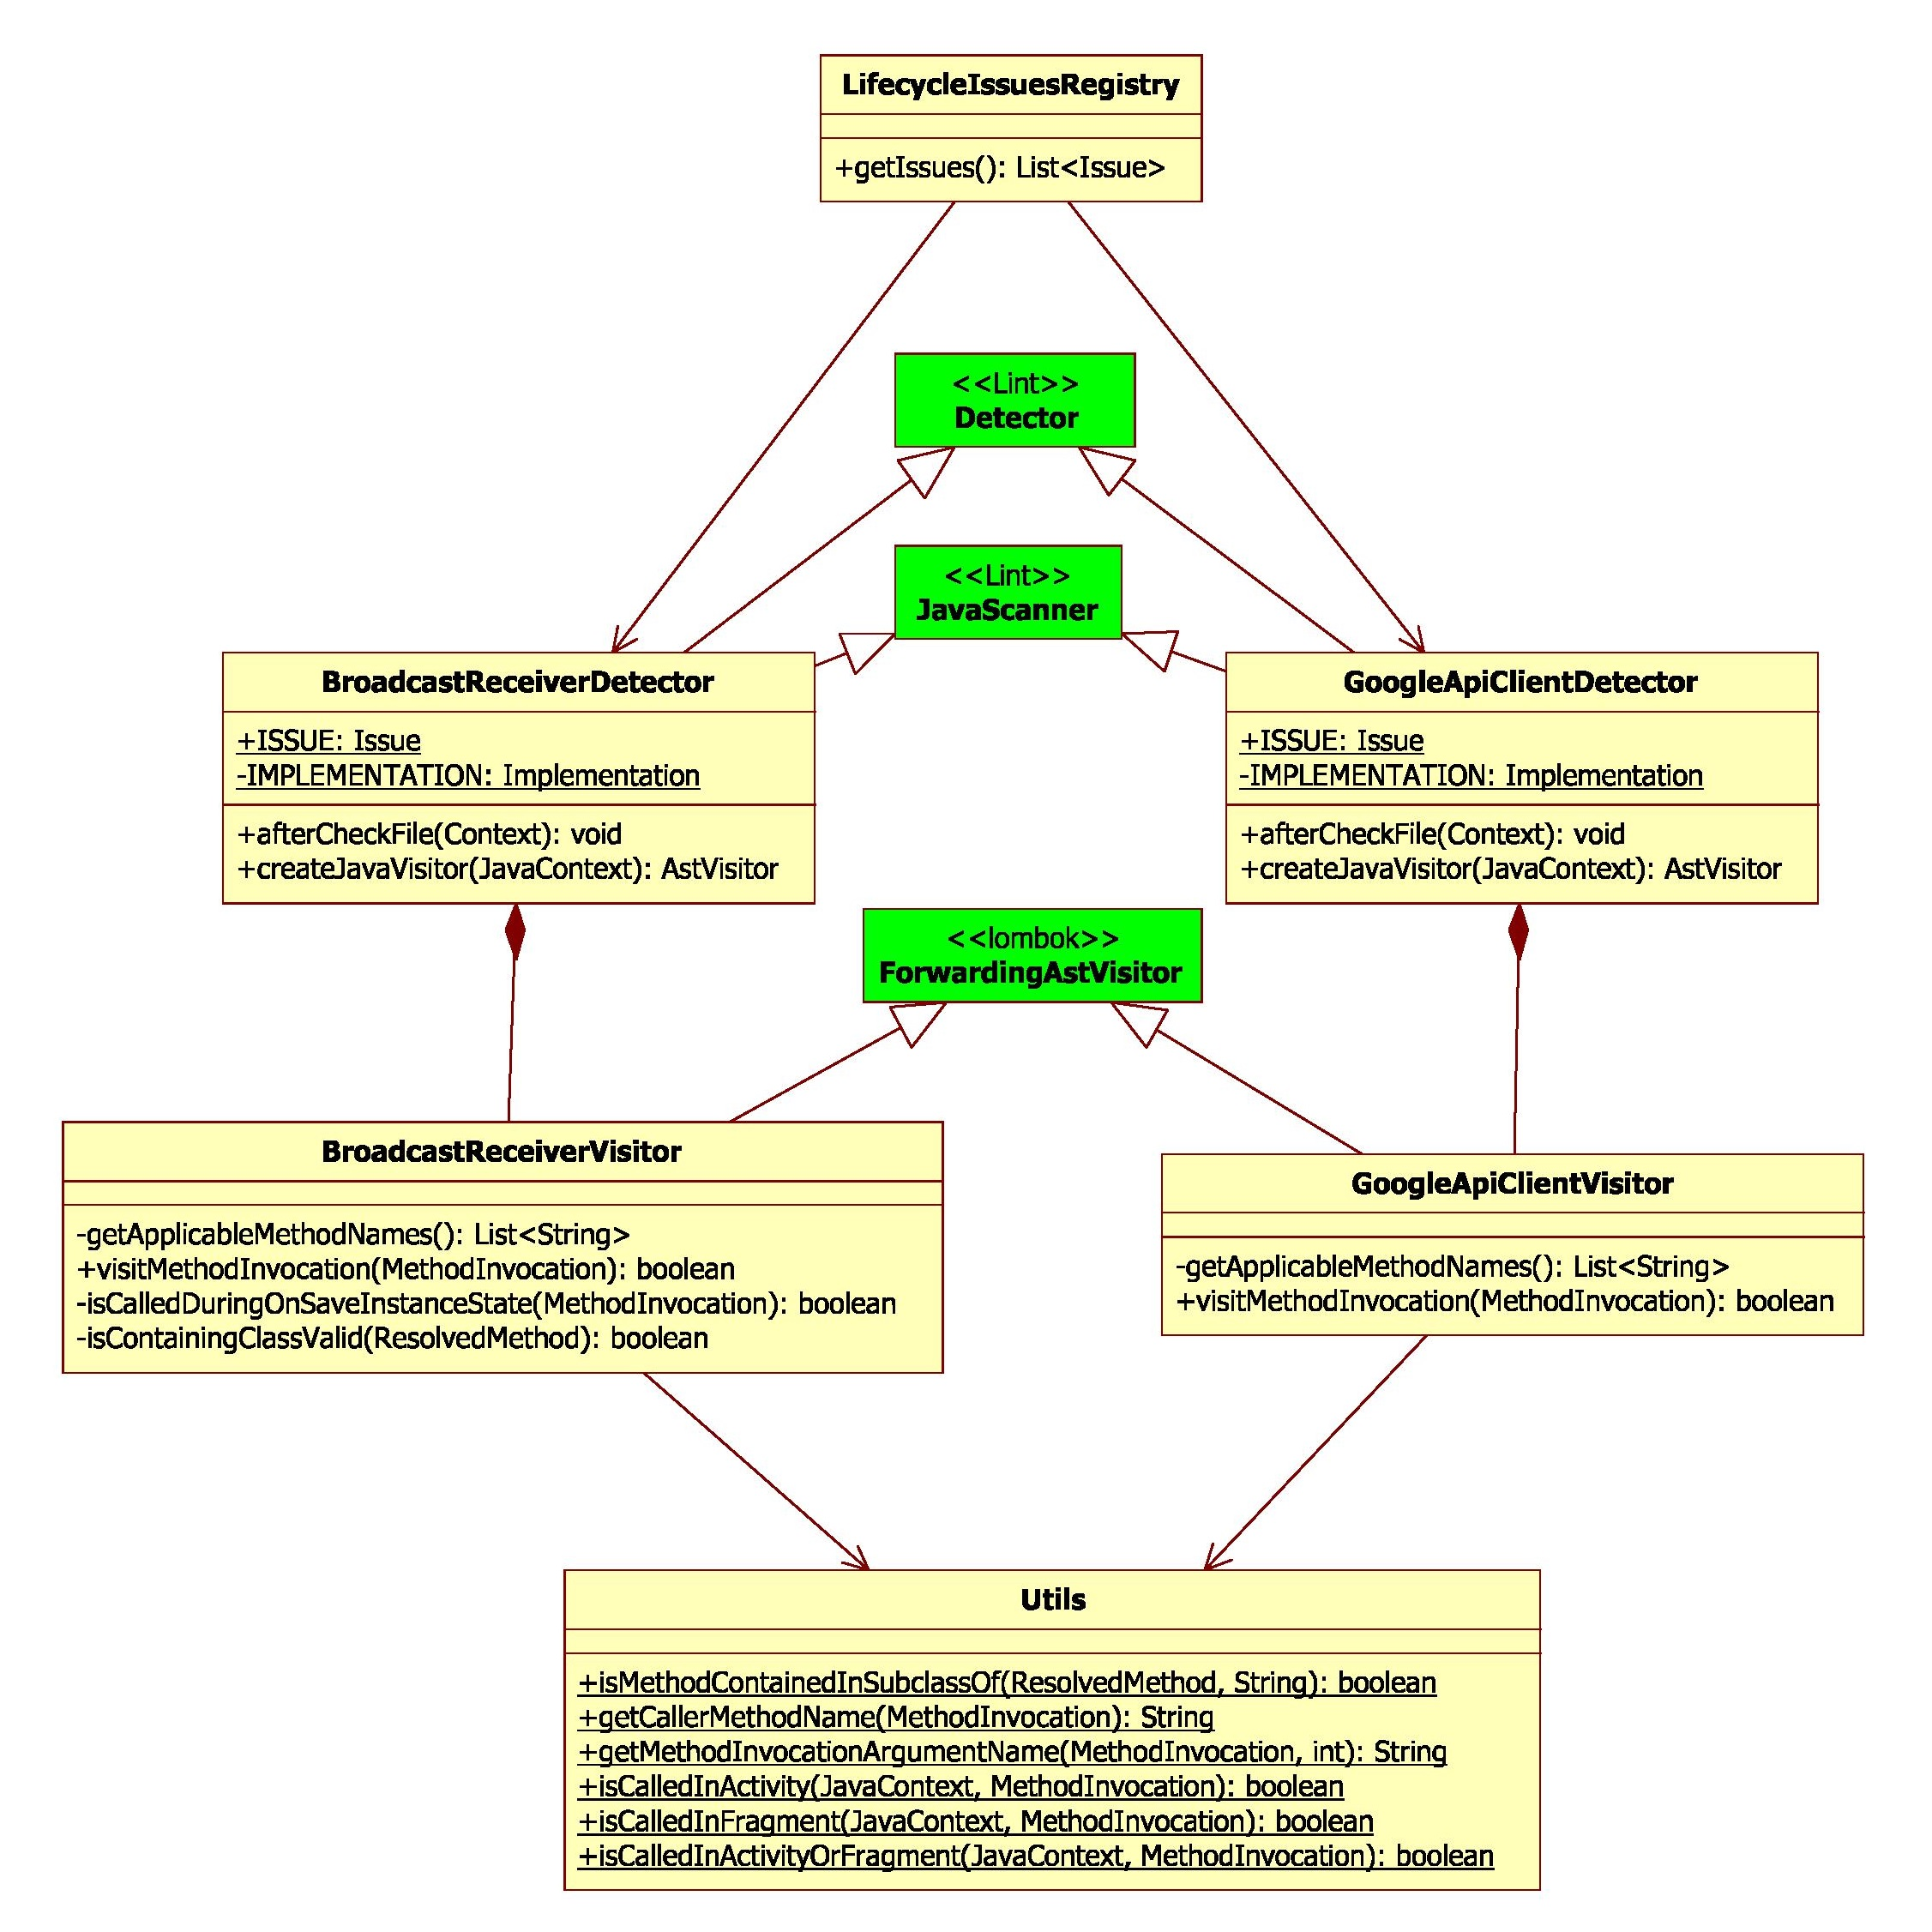
\includegraphics[width=\textwidth]{Images/LifecycleSta/UML/Implementation.jpg}
  \caption[Lifecycle Static Checks Implementation UML]{UML Diagram for the Lifecycle Static Checks Implementation}
\end{figure}
The detectors \texttt{BroadcastReceiverDetector} and \texttt{GoogleApiClientDetector} are implementations of \texttt{JavaScanner} and they both define a \texttt{ForwardingAstVisitor} subclass to implement their AST Traversal behavior.\medskip \\
In particular, \texttt{BroadcastReceiverVisitor} employs the \texttt{visitMethodInvocation(MethodInvocation)} callback to detect the calls to registration and unregistration. First, it checks that the current \texttt{MethodInvocation} is from the correct class (either \texttt{Context} for global receivers or \texttt{LocalBroadcastManager} for local receivers) and, if so, it stores the variable name in a list field variable. If it's the unregistration method, it also checks if the caller method is \texttt{onSaveInstanceState()} and in case shows a warning to the user. In the \texttt{afterCheckFile()} callback,  \texttt{BroadcastReceiverDetector} checks the stored values consistency, showing an issue if an unregistration is missing or if the same receiver is unregistered multiple times (without any try/catch block). In that case, it computes the code location handle to show a warning to the user in the correct place.\medskip \\
\texttt{GoogleApiClientVisitor} also receives the \texttt{visitMethodInvocation(MethodInvocation)} callback and checks if the current invocation is either a connection or a disconnection, setting a boolean flag for each. If the current class is an Activity or a Fragment, it checks that the caller method is \texttt{onStart()} or \texttt{onReceive()} respectively. During \texttt{afterCheckFile()}, the \texttt{GoogleApiClientDetector} shows a warning if the connection flag is set but the disconnection one is not, computing the correct location handle.\bigskip \\
Finally, the \texttt{LifecycleIssuesRegistry} simply sends the \texttt{Issue} objects (defined as static fields in the detector classes) to the Lint tool.

\fxnote*{New}{\subsection{Evaluation}}

\subsubsection{General Properties}
\begin{itemize}
	\item Applicability: the static lifecycle tests target a specific subset of Android applications, i.e. those that employ the components linked to each detector. Moreover, they are useful mostly in the early stages of development to recognize inconsistencies when the developer is coding a particular Activity or Fragment, since the issues would likely be detected at the first run or test case via crashes or logged errors.
	\item Effectiveness: static analysis in general can produce false negatives or false positives, so there may be situations where the developer is notified of a non-relevant problem or a real issue is not detected. For example, if the developer decides to employ the checked components in a non-standard way (e.g. register a Broadcast Receiver in an Activity and unregister it in another, passing the reference between them) the tool would wrongly recognize it as a problem.
	\item Usability: the static checks are completely integrated in the Lint tool available in the development IDE, so each of them behaves exactly as the built-in detectors. For this reason, the issues are both displayed as a visual clue on the code (the detected problem is highlighted and a warning message is shown) and they are included on the project-wide analysis run on demand by the developer.
	\item Performance: the Lint tool is usually able to analyze an entire project in a few seconds, checking for all the listed issues. The code of the developed lifecycle checks does not present any criticality from the performance point of view, since it employs only a AST Traversal technique on a single Java class.
\end{itemize}

\subsubsection{Real-World Application}
Since the lifecycle static checks are effective mostly in the early stages of development, it is not an easy task to find significant real-world examples of applications that may benefit from them. However, searching for open-source applications on the GitHub platform, the following examples may be found:
\begin{itemize}
	\item InTheClear~\cite{InTheClear} is an application for alerting during emergencies. Before commit \textit{cabfc26}\footnote{https://github.com/SaferMobile/InTheClear/commit/cabfc2643bc5820e109433a8ae48f9f6a0788d9f} a Broadcast Receiver was registered but never unregistered in the \texttt{SMSSender} class. Using the static lifecycle tests the developers would have detected the issue immediately, without the need to receive the log notification and open the issue \#56\footnote{https://github.com/SaferMobile/InTheClear/issues/56}.
	\item TrackBuddy~\cite{TrackBuddy} is an SMS tracker application. Commit \textit{007b6f7}\footnote{https://github.com/byteShaft/TrackBuddy/commit/007b6f7acb39e90d53ef38577d212927fae19d91} solves a bug in \texttt{LocationService}, which was missing a GoogleApiClient disconnection, a problem that would have been detected by lifecycle checks.
\end{itemize}

\section{Dynamic Analysis}\label{section_lifecycle_dynamic}

\subsection{Lifecycle Test Cases}
In this section a dynamic approach to lifecycle testing is presented, as opposed to the static technique described in the previous section.\medskip \\
The idea is to provide to the developer pre-generated test cases that allow to explore the most common lifecycle changes, to overcome the limitation of the built-in testing frameworks that only provide low-level methods that need to be carefully chained each time. With the proposed approach, the complexity of managing the lifecycle transitions is completely hidden to the developer, which can only focus on expressing actions to be performed and conditions to be checked during the test execution.

\subsection{Design}
To allow custom actions and checks during the pre-defined lifecycle tests the system uses several callbacks, for example the \textit{PauseCallback} allows the developer to specify some actions and checks before the component is paused, some checks while it is paused and some other actions and checks when the component is resumed again. These callbacks are defined by the developer inside a test case and then used by the system during the actual lifecycle tests in the appropriate moments.\medskip \\
The pre-generated lifecycle tests are defined for two frameworks:
\begin{itemize}
	\item Activity Test Rule tests: the \texttt{ActivityTestRule} objects allow the developer to specify which Activity to consider during a test. It is used for:
	\begin{itemize}
		\item Instrumented unit testing
		\item Espresso UI testing
	\end{itemize}
	\item Robolectric tests: "hybrid" unit testing
\end{itemize}
Which cover the most used modern testing mechanisms in Android.\bigskip \\
The defined tests are:
\begin{itemize}
	\item Pause: simulates the component being partially hidden, i.e. paused and then resumed. It is useful for example to see if the component correctly frees/stops and reacquires/starts "critical" resources and CPU-intensive operations.
	\begin{itemize}
		\item \texttt{onCreate()}
		\item \texttt{onStart()}
		\item \texttt{onResume()}
		\item \textit{Actions and assertions before the pause}
		\item \texttt{onPause()}
		\item \textit{Assertions while paused}
		\item \texttt{onResume()}
		\item \textit{Actions and assertions after the pause}
	\end{itemize}
	\item Stop: simulates the component being completely hidden (in background), i.e. stopped and restarted. The developer can for example check if all resources used by the application are correctly released while the component is in background, to avoid wasting computational power.
	\begin{itemize}
		\item \texttt{onCreate()}
		\item \texttt{onStart()}
		\item \texttt{onResume()}
		\item \textit{Actions and assertions before the stop}
		\item \texttt{onPause()}
		\item \texttt{onStop()}
		\item \textit{Assertions while stopped}
		\item \texttt{onRestart()}
		\item \texttt{onStart()}
		\item \texttt{onResume()}
		\item \textit{Actions and assertions after the stop}
	\end{itemize}
	\item Destruction: simulates the component being closed (e.g. back button pressed or the application is killed by the system). In this case two different tests are defined, one where \texttt{onDestroy()} is called and another one where it is not, since in a real application this call is not guaranteed\footnote{https://developer.android.com/reference/android/app/Activity.html\#onDestroy()}. This test case can be used for example to see if the component stops all computations and, if needed, stores unsaved data in memory.
	\begin{itemize}
		\item \texttt{onCreate()}
		\item \texttt{onStart()}
		\item \texttt{onResume()}
     	\item \textit{Actions and assertions before the destruction}
		\item \texttt{onPause()}
		\item \texttt{onStop()}
		\item $[$\texttt{onDestroy()}$]$
     	\item \textit{Assertions after the destruction}
	\end{itemize}
	\item Recreation: simulates the component being recreated. This can happen for example when a device configuration change happens (e.g. device is rotated) or an application in background is killed by Android to free resources and then restarted. This is usually the most critical lifecycle transition: since a completely new instance of the component is created (with a different reference), all variables that are not passed in the saved instance state \texttt{Bundle} are lost, other components (e.g. \texttt{AsyncTask}) may not be able to commit their results to the new component, etc.  
	\begin{itemize}
		\item \texttt{onCreate()}
		\item \texttt{onStart()}
		\item \texttt{onResume()}
     	\item \textit{Actions and assertions before the recreation}
		\item \texttt{onPause()}
		\item \texttt{onStop()}
		\item \texttt{onDestroy()}
		\item \texttt{onCreate()}
		\item \texttt{onStart()}
		\item \texttt{onResume()}
     	\item \textit{Actions and assertions after the recreation}
	\end{itemize}
	The test case also provides a way to check the actual contents of the saved instance state \texttt{Bundle} to see if it contains the correct data passed from the old to the new instance of the component.
	\item Rotation: simulates the device being rotated, from portrait to landscape modes or vice versa. By default, from the lifecycle point of view this has the same effect of a recreation, but the developer can specify a different behavior changing the \texttt{configChanges} attribute in the application manifest. This test case can be useful to see if the component dynamically adapts to the new rotation, e.g. providing a different UI layout.
	\begin{itemize}
		\item \texttt{onCreate()}
		\item \texttt{onStart()}
		\item \texttt{onResume()}
		\item \textit{Actions and assertions before the rotation}
		\item $[$Possible lifecycle changes, by default recreation$]$
		\item \textit{Actions and assertions after the rotation}
	\end{itemize}
\end{itemize}
The developer can also chain several of the listed tests together to build a complex execution flow, for example first pausing and resuming an Activity, and then destroying it.

\subsection{Implementation}
\begin{figure}
  \centering
  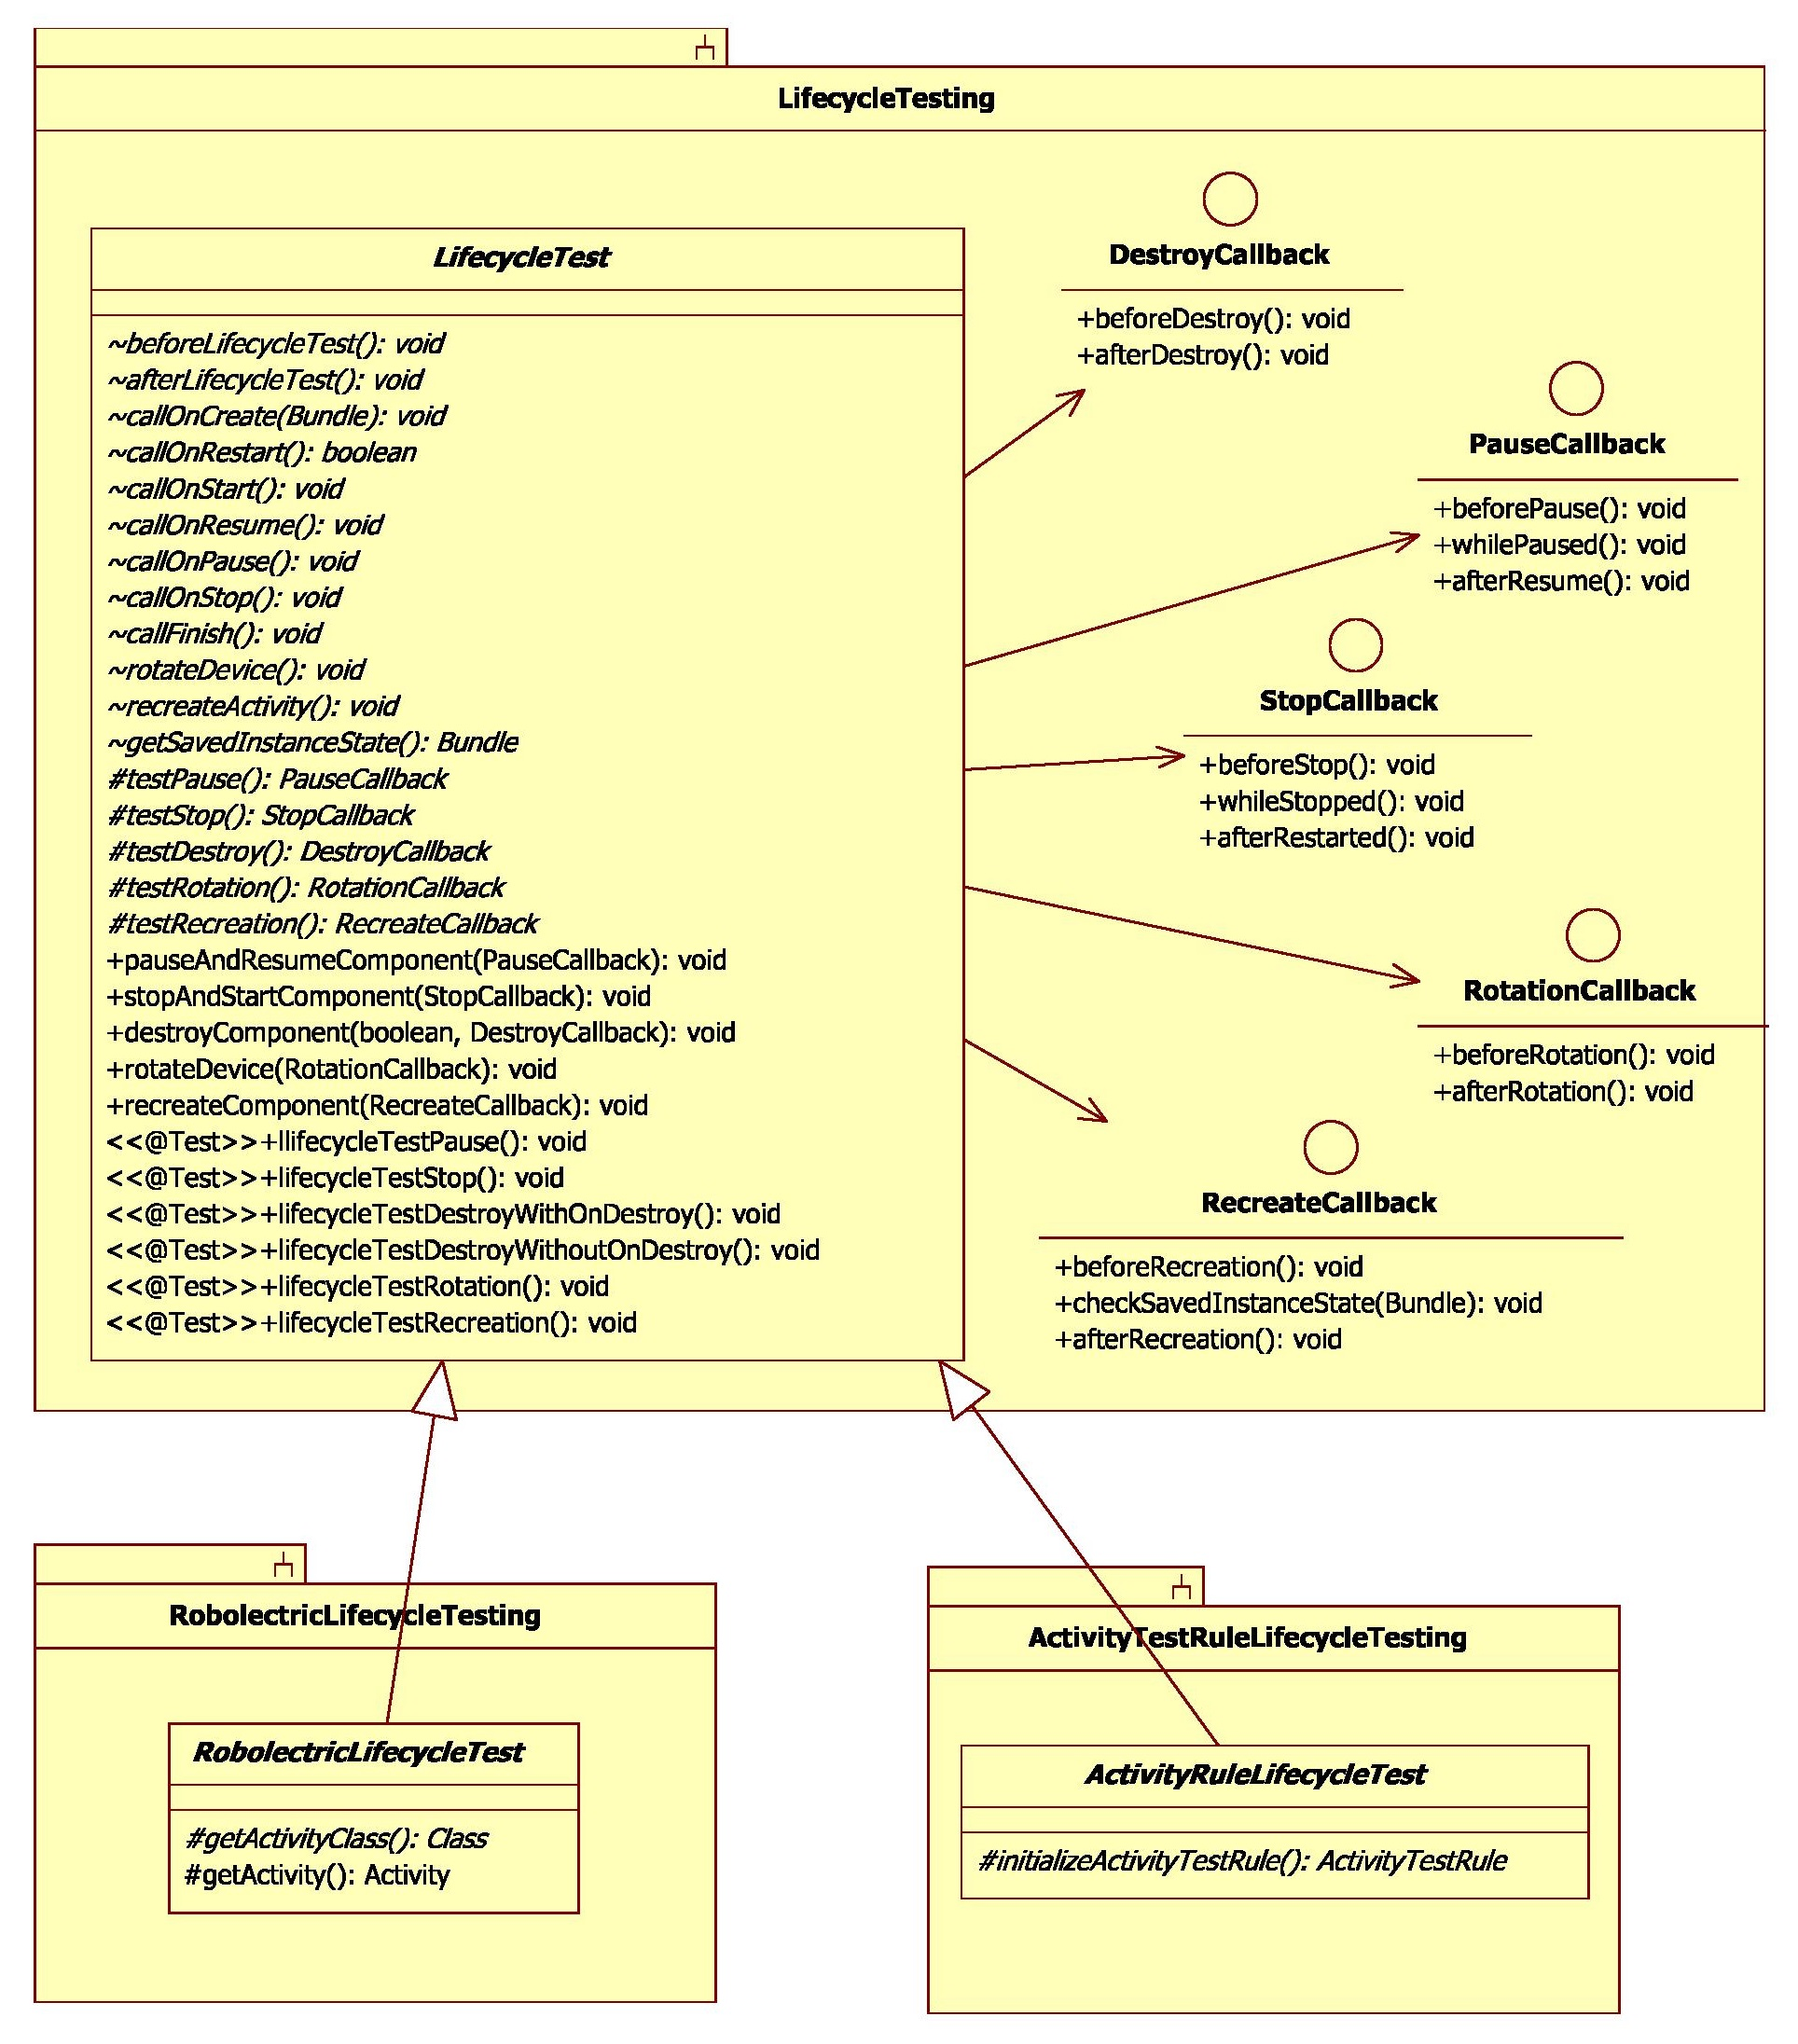
\includegraphics[width=\textwidth]{Images/LifecycleDyn/UML/Implementation.jpg}
  \caption[Lifecycle Tests Implementation UML]{UML Diagram for the Lifecycle Dynamic Tests Implementation}
\end{figure}
The dynamic lifecycle tests library~\cite{DynamicLifecycleTesting} is split in three modules. The reason for this is the Android system of including test libraries: using Gradle, the developer can \textit{testCompile} the libraries used for local tests (i.e. that run on the development computer) and \textit{androidTestCompile} the libraries used for instrumented tests (i.e. that run on real mobile devices or emulators). Since Robolectric is local and Activity Test Rule is instrumented, two distinct modules \texttt{RobolectricLifecycleTesting} and \texttt{ActivityTestRuleLifecycleTesting} allow the developer to correctly include them without creating useless dependencies. The module \texttt{LifecycleTesting} includes the common parts of the other two.\medskip \\
The \texttt{LifecycleTest} class inside the \texttt{LifecycleTesting} module is the main class of the system. It defines:
\begin{itemize}
	\item Abstract methods implemented by the sub-modules that allow to specify the means to control the component lifecycle, according to their structure.
	\item Abstract methods implemented by the end-developer that allow to pass the callbacks for each lifecycle test.
	\item Helper methods that define the correct sequence of lifecycle callbacks for each of the tests, which can also be used by the end-developer to chain several test cases together.
	\item The actual tests that use the previous three sets of methods to drive the lifecycle and to perform actions and checks in between.
\end{itemize}
Inside the module, several interfaces for the callbacks are also defined. \bigskip \\
The \texttt{RobolectricLifecycleTest} class inside the  \texttt{RobolectricLifecycleTesting} module is the implementation of the lifecycle tests for the Robolectric framework. Besides implementing the methods to drive the component lifecycle using the Robolectric \texttt{ActivityController} class, it also provides the abstract method \texttt{getActivityClass()} to allow the developer to define the activity under test and the utility \texttt{getActivity()} that allows to retrieve the activity during a callback.\bigskip \\
Activity Test Rule tests are covered by the \texttt{ActivityRuleLifecycleTest} class inside the \texttt{ActivityTestRuleLifecycleTesting} module. It implements the lifecycle methods using the Android \texttt{Instrumentation} class and provides the abstract method \texttt{initializeActivityTestRule()} to allow the developer to define the Activity Test Rule under test.

\fxnote*{New}{\subsection{Evaluation}}

\subsubsection{General Properties}
\begin{itemize}
	\item Applicability: lifecycle tests have a wide applicability range, since the behavior of almost every Activity of an application is directly affected by its lifecycle. Moreover, the tests are available for Activity Test Rule unit/integration testing, Espresso UI testing and Robolectric unit testing, and so they can be applied in most of the testing environments employed in Android development.
	\item Effectiveness: the tests correctly simulate the real behaviors of lifecycle transitions, allowing the developer to setup test cases that can effectively reveal criticalities.
	\item Usability: to define the lifecycle test cases the developer only needs to inherit from the classes provided by the library and implement the abstract methods. In each of them, the complexity of handling the lifecycle transitions is completely hidden to the developer thanks to the callback mechanism, allowing to focus only on the actions and assertions to be performed during the test.
	\item Performance: the overhead introduced by the lifecycle transitions handling is negligible, and so the time complexity of each test depends only on the actions and assertions defined by the developer.
\end{itemize}

\subsubsection{Real-World Application} \fix{Do you provide listings of the generated tests? If not, could you please add short code snippets showing how your tests will look like for the three cases. And mention if developers have added any new test cases.}
To prove the lifecycle tests effectiveness, the library has been applied to WordPress~\cite{WordPressApp}, the Android application that allows to manage directly from mobile devices the websites created with the well-known content management system WordPress~\cite{WordPressCMS}.\bigskip \\ \fix{to separate paragraphs just an empty line in the latex source should be enough. Without \texttt{bigskip} etc.}

The evaluation has been performed by applying the same lifecycle tests first on an old version of the application (at commit \textit{9f9cb12}\footnote{https://github.com/wordpress-mobile/WordPress-Android/commit/9f9cb12bb1d8a82d60897b5c3ff954c2f88de4f2} on December 6, 2015)~\cite{WordPress2015-12-06} and then on the latest version at the time of writing (at commit \textit{bfdf611}\footnote{https://github.com/wordpress-mobile/WordPress-Android/commit/bfdf611c6a37ddd1fad1980f73a00389b2e22677} on July 15, 2016)~\cite{WordPress2016-07-15}. In the six months elapsed between the two versions some lifecycle issues were discovered and fixed, and so the idea is to show that the defined tests fail in the older version while they succeed in the newer one.\bigskip \\
The defined tests are:
\begin{itemize}
	\item Loss of data in profile
	\begin{itemize}
		\item Bug Category: usability, correctness
		\item Lifecycle Transition: rotation
		\item Linked Issue: \#3608\footnote{https://github.com/wordpress-mobile/WordPress-Android/issues/3608}
		\item Fixed In: pull request \#3912\footnote{https://github.com/wordpress-mobile/WordPress-Android/pull/3912} 
		\item Problem Description: in the profile page, if the user typed a value (e.g. his/her name) and then rotated the device, the inserted data would be lost.
		\item Test: the lifecycle test, defined in Espresso, exploits the rotation callback by first typing the name value and then, after the transition, asserting the input contents. The source code of the test can be found in listing~\ref{lst_lifecycle_wp}.
		\item Causes and Solutions: the bug was caused by not saving the instance of the views at the device rotation. The chosen solution was to employ a \texttt{DialogFragment} component that automatically manages button and dialog, including their lifecycle.
	\end{itemize}
	\item Blank post content
	\begin{itemize}
		\item Bug Category: correctness
		\item Lifecycle Transition: pause/stop
		\item Linked Issue: \#3575\footnote{https://github.com/wordpress-mobile/WordPress-Android/issues/3575}
		\item Fixed In: pull request \#3577\footnote{https://github.com/wordpress-mobile/WordPress-Android/pull/3577} 
		\item Problem Description: reading a long blog post, pausing and resuming the application caused most of the content to be invisible to the user.
		\item Test: the Espresso lifecycle test opens a blog post, scrolls down and, after the pause, checks that all the content is displayed.
		\item Causes and Solutions: the \texttt{WebView} component used to display the page was paused during \texttt{onPause()} but not resumed during \texttt{onResume()}, and so the simple solution of the bug was to add the latter call.
	\end{itemize}
	\item Unexpected page change
	\begin{itemize}
		\item Bug Category: usability
		\item Lifecycle Transition: rotation
		\item Linked Issue: \#3948\footnote{https://github.com/wordpress-mobile/WordPress-Android/issues/3948}
		\item Fixed In: pull request \#4127\footnote{https://github.com/wordpress-mobile/WordPress-Android/pull/4127} 
		\item Problem Description: in the settings page, if the user accessed the notifications-specific area and then rotated the device, he/she was redirected back to the general settings screen. 
		\item Test: the Espresso lifecycle test first opens the settings page and clicks on the notifications section button, then after the rotation checks if the same page is still displayed.
		\item Causes and Solutions: the bug was caused by the missing \texttt{NotificationsSettingsActivity} rotation handling. To solve the issue, the developers decided to simply add \texttt{android:configChanges=\char`\"orientation|screenSize\char`\"} in the application manifest, to override the automatic recreation of the Activity after the rotation. This solution was chosen for consistency with the other Activities of the application, but it is not ideal since the Android developers themselves suggest it only as a last resort\footnote{https://developer.android.com/guide/topics/manifest/activity-element.html}.
	\end{itemize}
\end{itemize}


%..............................................................................%
%.................................... EVENTS ..................................%
%..............................................................................%

\newpage
\part{Event-based Testing}\label{part_events}

\section{Introduction}
Moving from the specific type of events related to the lifecycle to a more general concept of event, we can also state that the built-in testing support is lacking from this point of view. In general, the only way to test concurrency of events with the provided frameworks is to manually set variables and check their state via conditional statements, which hardly helps in complex environments.\medskip \\
Given this lack of testing capabilities, several approaches related to the issue of race conditions were devised. These tools, like dynamic analysis with EventRacer and static analysis with DEvA, described in detail in section \ref{section_race_tools}, do not focus on manual testing but on automatic detection of concurrency problems among events, mainly related to data races.\medskip \\
The solution proposed in the second part of this thesis aims at being a complementary tool to these approaches. Instead of focusing on automatic detection, it provides the means to manually specify event-related conditions during standard unit, integration or UI tests. This means that this approach presents the advantage of avoiding the issue of false positives and false negatives, intrinsic for detection tools, but the developer has to code test cases by hand to cover the relevant parts of the application.\medskip \\
More in detail, with the proposed event-based testing library the developer is able to specify which events to observe during the execution of the application and then to define consistency checks on their stream, such as happens-before relationship, ordering and existence.\medskip \\
This approach allows to detect possible race conditions like the other tools, but the scope is not limited to data races: the developer is able to specify any type of condition on any event generated by the application, from user input to sensor data callbacks. Moreover, the tool does not only apply to race conditions but it also allows to focus on ordering among similar events, to quantify the amount of events of a certain type during a particular execution and so on.\medskip \\
The implementation of this event-based testing approach exploits the ReactiveX library, an innovative system of industrial interest (it is employed for example by Microsoft and Netflix) that allows to observe, transform and listen to events.\medskip \\
The following sections first present a formalization of the temporal assertions language used to define the consistency checks on the event stream, followed by a detailed explanation of the design, implementation and evaluation of the system.

\section{Temporal Assertions Language}

\subsection{Consistency Checks}
An approach to event-based testing is to define consistency checks, i.e. conditions that should be verified in the event stream. For example we can define the happens-before relationship between two or more events, specify the exact number of events of a certain type that can appear during a particular execution and so on.\medskip \\
The idea of event-based testing described in this part of the thesis is based on a temporal assertions language: a language that allows to express consistency checks on some of the events generated during the application execution and, in case they are not satisfied, the assertion error is notified to the developer. A detailed explanation of the language to express checks is reported in the next sections.\bigskip \\
First, let's formally define some terminology:
\begin{itemize}
	\item Event Stream $E$: the list of all the events registered during a particular execution, i.e. from the tool start at time \textit{t1} until the tool stop at time \textit{t2}.
	\item Event $e \in E$: an event contained in the stream. The event stream is totally ordered: each event has a generation time and given any two events $e1$ and $e2$ we have either $e1 \prec e2$ or $e2 \prec e1$.
	\item Consistency Check $c$: a rule among one or more events that should be verified in the stream. Once specified, the check is applied to the stream and returns either a \textit{Success} or \textit{Failure} outcome.
	\item Matcher $m$: a specification that describes one or more events in the stream. It is used by the consistency checks to match the events, in order to express a condition on them. For example, considering the events to be names, if $E= \big\{ John, Bill, Mary, Jack, Elizabeth \big\} $, the matcher $starts\_with\_J$ would match (i.e. return true) the events $John$ and $Jack$.
	\item $n, i \in \mathbb{N}$
\end{itemize}\medskip
In the proposed formalization, each check is described by:
\begin{itemize}
	\item Code structure: abstract description of the check specification. It has the same structure of the final code but use the aforementioned terminology to describe which components are expected.
	\item Description: a brief explanation of the check logic.
	\item First Order Logic (FOL) formalization of the check meaning, expressed using the following logic relationships:
	\begin{itemize}
		\item $match(e, m)$ means that the matcher \textit{m} matches the event \textit{e}.
		\item $before(e1, e2)$ means that the event \textit{e1} is generated in the sequence before \textit{e2}, i.e. $e1 \prec e2$.
		\item $between(e2, e1, e3) \equiv before(e2, e1) \land before(e1, e3)$ means that the event \textit{e1} is generated in the sequence after \textit{e2} and before \textit{e3}, i.e. $e2 \prec e1 \prec e3$.
	\end{itemize}
	\item Visual representation: shows some examples of event streams and the corresponding check outcome. The outcome is placed in the spot where it is actually produced by the system: some checks may not need to explore the whole stream, i.e. if the condition is fulfilled or violated after an intermediate event the check "short-circuits".
	\item Real code example: an example of check specification as implemented by the system. The structure of the Java classes and objects will be clear later when the implementation is explained in detail.
\end{itemize}


\subsection{Checks on Single Events}

The first type of checks focuses on single events at a time: for example we may say that an event of a certain type can be detected in the stream only after another event of a certain type.

\subsubsection{Can Happen Only After}

\begin{center}
\bgroup
\def\arraystretch{1.5}%
\begin{longtable}{ | m{0.3cm} | m{15cm} | }
  \hline
  
  \rotatebox[origin=c]{90}{\textbf{ Structure }} & 
  
  	\begin{lstlisting}
	anEventThat(m1).canHappenOnlyAfter(anEventThat(m2))
	\end{lstlisting}
	
  	\\ \hline
  	 
  \rotatebox[origin=c]{90}{\textbf{ Description }} & 
  
  	Checks that the events that match \texttt{m1} happen only after any event that matches \texttt{m2}, i.e. there cannot be an event that matches \texttt{m1} before the first event that matches \texttt{m2}.
	
  	\\ \hline

  \rotatebox[origin=c]{90}{\textbf{ FOL }} & 
  
  	\begin{multline*}
\forall e1 \bigg( match(e1, m1) \Rightarrow \exists e2 \Big( match(e2, m2) \land before(e2, e1) \Big) \bigg)
	\end{multline*}
	
  	\\ \hline

  \rotatebox[origin=c]{90}{\textbf{ Visual }} & 
  
	\raisebox{-230pt}{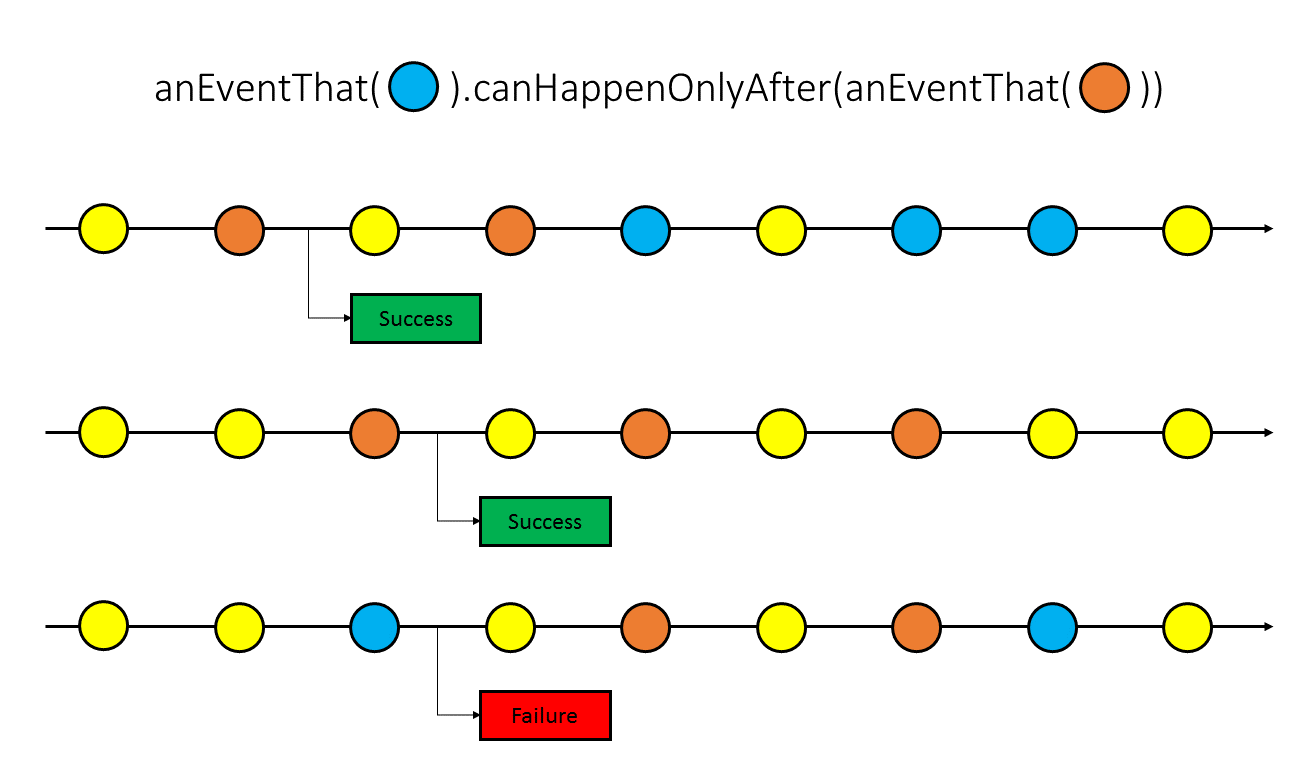
\includegraphics[width=400px]{Images/Event/Lang/Slide1.PNG}}
	
	Note in particular that in the second case the checks succeeds even if no blue event occurs: we are  just saying that blue events \textit{can} happen after an orange one.
	
  	\\ \hline
  	
  \rotatebox[origin=c]{90}{\textbf{ Code Example }} & 
  
  	\begin{lstlisting}
	/* Check race condition with maps */
	anEventThat(isMarkerPlacement())
		.canHappenOnlyAfter(anEventThat(isMapReady()));
	\end{lstlisting}
	
  	\\ \hline  	
  	 
\end{longtable}
\egroup
\end{center}

\subsubsection{Can Happen Only Before}

\begin{center}
\bgroup
\def\arraystretch{1.5}%
\begin{longtable}{ | m{0.3cm} | m{15cm} | }
  \hline
  
  \rotatebox[origin=c]{90}{\textbf{ Structure }} & 
  
  	\begin{lstlisting}
	anEventThat(m1).canHappenOnlyBefore(anEventThat(m2))
	\end{lstlisting}
	
  	\\ \hline
  	 
  \rotatebox[origin=c]{90}{\textbf{ Description }} & 
  
  	Checks that the events that match \texttt{m1} happen only before any event that matches \texttt{m2}, i.e. there cannot be an event that matches \texttt{m1} after the last event that matches \texttt{m2}.
	
  	\\ \hline

  \rotatebox[origin=c]{90}{\textbf{ FOL }} & 
  
  	\begin{multline*}
	\forall e1 \bigg( match(e1, m1) \Rightarrow \exists e2 \Big( match(e2, m2) \land before(e1, e2) \Big) \bigg)
	\end{multline*}
	
  	\\ \hline

  \rotatebox[origin=c]{90}{\textbf{ Visual }} & 
  
	\raisebox{-230pt}{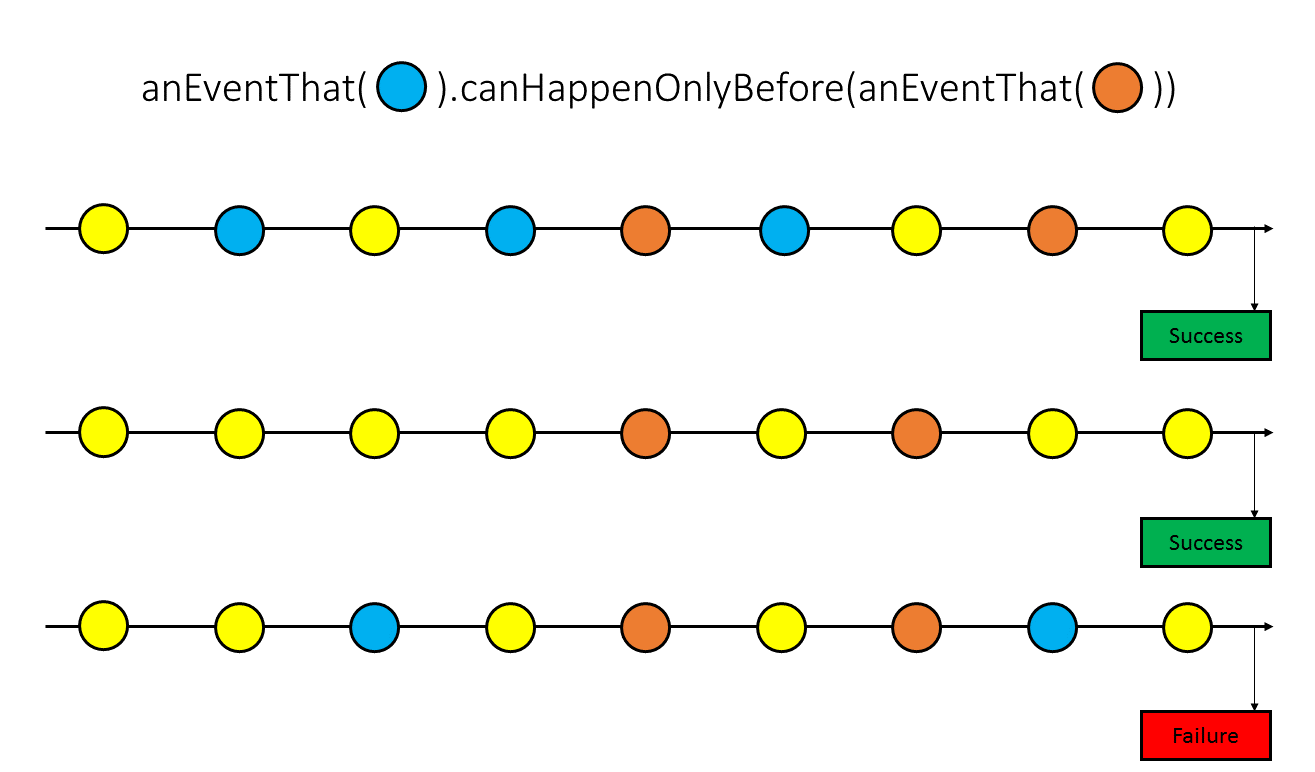
\includegraphics[width=400px]{Images/Event/Lang/Slide2.PNG}}
	
	
  	\\ \hline
  	
  \rotatebox[origin=c]{90}{\textbf{ Code Example }} & 
  
  	\begin{lstlisting}
	/* Can change form input only before it is submitted */
	anEventThat(isTextChangeFrom(usernameTextView))
		.canHappenOnlyBefore(anEventThat(isSubmitForm()));
	\end{lstlisting}
	
  	\\ \hline  	
  	 
\end{longtable}
\egroup
\end{center}

\subsubsection{Can Happen Only Between}

\begin{center}
\bgroup
\def\arraystretch{1.5}%
\begin{longtable}{ | m{0.3cm} | m{15cm} | }
  \hline
  
  \rotatebox[origin=c]{90}{\textbf{ Structure }} & 
  
  	\begin{lstlisting}
	anEventThat(m1).canHappenOnlyBetween(anEventThat(m2), anEventThat(m3))
	\end{lstlisting}
	
  	\\ \hline
  	 
  \rotatebox[origin=c]{90}{\textbf{ Description }} & 
  
  	Checks that the events that match \texttt{m1} happen only between an event that matches \texttt{m2} and an event that matches \texttt{m3}, i.e. there cannot be an event that matches \texttt{m1} outside a pair \texttt{m2}-\texttt{m3}. 
	
  	\\ \hline

  \rotatebox[origin=c]{90}{\textbf{ FOL }} & 
  
  	\begin{multline*}
	\forall e1 \Bigg( match(e1, m1) \Rightarrow \exists e2, e3 \bigg( match(e2, m2) \land match(e3, m3) \\ \land between(e2, e1, e3) \land \neg \exists e3' \Big( match(e3', m3) \land \big( between(e2, e3', e1) \\ \lor between(e1, e3', e3) \big) \Big) \bigg) \Bigg)
	\end{multline*}
	
  	\\ \hline

  \rotatebox[origin=c]{90}{\textbf{ Visual }} & 
  
	\raisebox{-230pt}{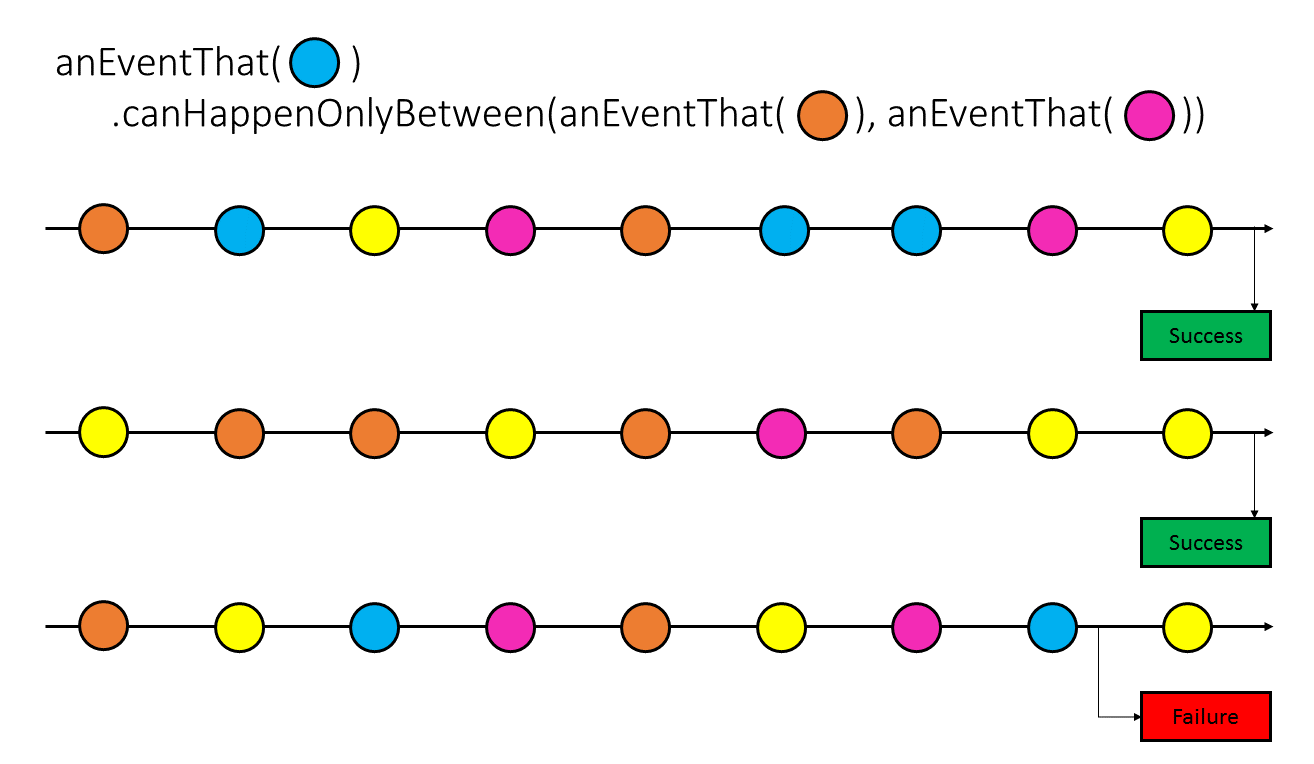
\includegraphics[width=400px]{Images/Event/Lang/Slide3.PNG}}
	
	
  	\\ \hline
  	
  \rotatebox[origin=c]{90}{\textbf{ Code Example }} & 
  
  	\begin{lstlisting}
	/* Can send broadcast only if the service is working */
	anEventThat(isSendBroadcast())
		.canHappenOnlyBetween(
			anEventThat(isServiceStart(mainService)),
			anEventThat(isServiceStop(mainService)));
	\end{lstlisting}
	
  	\\ \hline  	
  	 
\end{longtable}
\egroup
\end{center}

\subsection{Checks on Sets of Events}

These checks work on sets of events: for example we may say that a certain event generates a set of \textit{n} other events. The cardinality of each set is specified by the quantifiers:
\begin{itemize}
	\item Exactly
	\item At most
	\item At least
\end{itemize}
Only the formulas for "exactly" are written since the others can be derived by analogy.\bigskip \\
First Order Logic specifications use the counting quantifiers~\cite{Pratt-Hartmann:2014:LCE:2603088.2603117} as a notational shorthand, i.e. $\exists_{=n} x$ means that there exist exactly \textit{n} elements \textit{x}.

\subsubsection{Must Happen After}

\begin{center}
\bgroup
\def\arraystretch{1.5}%
\begin{longtable}{ | m{0.3cm} | m{15cm} | }
  \hline
  
  \rotatebox[origin=c]{90}{\textbf{ Structure }} & 
  
  	\begin{lstlisting}
	exactly(n).eventsWhereEach(m1).mustHappenAfter(anEventThat(m2))
	\end{lstlisting}
	
  	\\ \hline
  	 
  \rotatebox[origin=c]{90}{\textbf{ Description }} & 
  
  	Checks that exactly \texttt{n} events that match \texttt{m1} happen exclusively after every event that matches \texttt{m2}. "Exclusively" means that there cannot be another event that matches \texttt{m2} before the sequence of \texttt{n} events is completed.
	
  	\\ \hline

  \rotatebox[origin=c]{90}{\textbf{ FOL }} & 
  
  	\begin{multline*}
	\forall e2 \Bigg( match(e2, m2) \Rightarrow \exists_{=n} e1 \bigg( match(e1, m1) \land before(e2, e1) \\ \land \neg \exists e2' \Big( match(e2', m2) \land between(e2, e2', e1) \Big) \bigg) \Bigg)
	\end{multline*}
	
  	\\ \hline

  \rotatebox[origin=c]{90}{\textbf{ Visual }} & 
  
	\raisebox{-280pt}{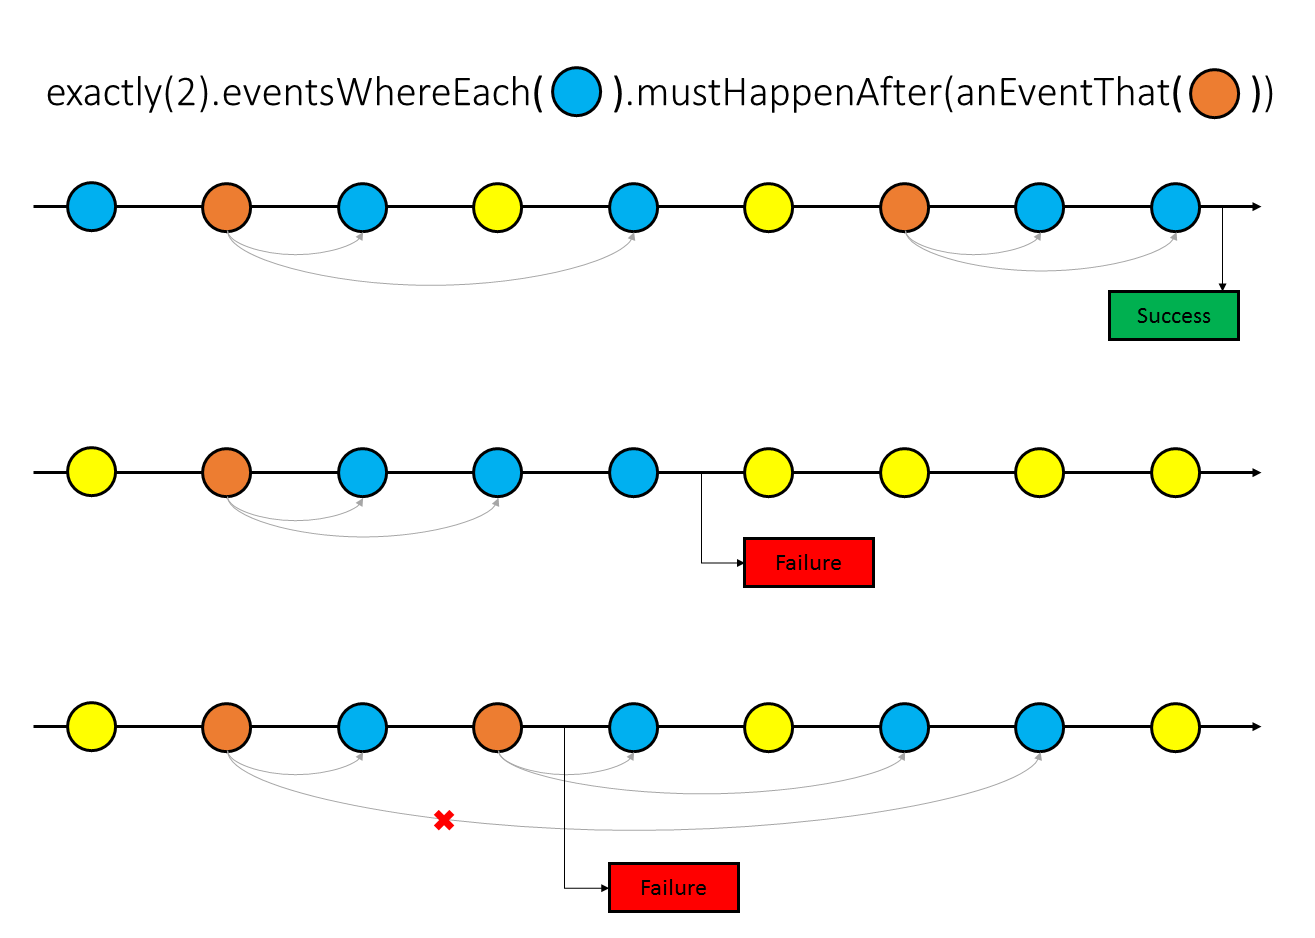
\includegraphics[width=400px]{Images/Event/Lang/Slide4.PNG}}
	
	Note in particular that the third case shows the "exclusively" constraint mentioned before: the check fails because we do not have two blue events after the first orange but before the second one (i.e. the first orange event does \textit{not} match one of the three blue events that follow the second orange event).

  	\\ \hline
  	
  \rotatebox[origin=c]{90}{\textbf{ Code Example }} & 
  
  	\begin{lstlisting}
	/* If a location change happens, the text view must be updated exactly once */	
	exactly(1).eventsWhereEach(isTextChangeFrom(locationTextView))
		.mustHappenAfter(anEventThat(isLocationChange()));
	\end{lstlisting}
	
  	\\ \hline  	
  	 
\end{longtable}
\egroup
\end{center}

\subsubsection{Must Happen Before}

\begin{center}
\bgroup
\def\arraystretch{1.5}%
\begin{longtable}{ | m{0.3cm} | m{15cm} | }
  \hline
  
  \rotatebox[origin=c]{90}{\textbf{ Structure }} & 
  
  	\begin{lstlisting}
	exactly(n).eventsWhereEach(m1).mustHappenBefore(anEventThat(m2))
	\end{lstlisting}
	
  	\\ \hline
  	 
  \rotatebox[origin=c]{90}{\textbf{ Description }} & 
  
  	Checks that exactly \texttt{n} events that match \texttt{m1} happen exclusively before every event that matches \texttt{m2}. "Exclusively" means that the sequence of \texttt{n} events must be after the previous (if any) event that matches \texttt{m2}.
	
  	\\ \hline

  \rotatebox[origin=c]{90}{\textbf{ FOL }} & 
  
  	\begin{multline*}
	\forall e2 \Bigg( match(e2, m2) \Rightarrow \exists_{=n} e1 \bigg( match(e1, m1) \land before(e1, e2) \\ \land \neg \exists e2' \Big( match(e2', m2) \land between(e1, e2', e2) \Big) \bigg) \Bigg)
	\end{multline*}
	
  	\\ \hline

  \rotatebox[origin=c]{90}{\textbf{ Visual }} & 
  
	\raisebox{-280pt}{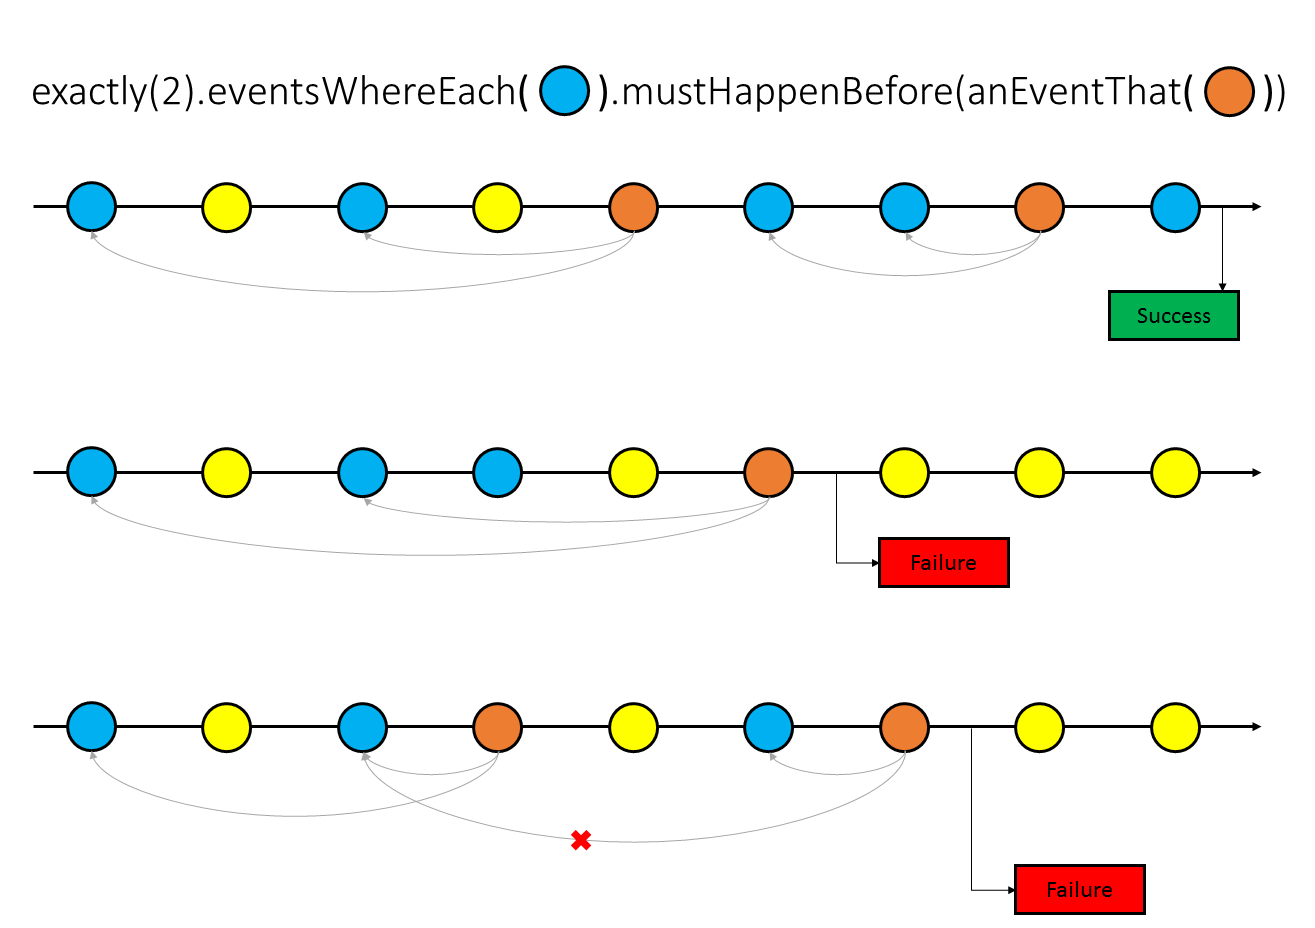
\includegraphics[width=400px]{Images/Event/Lang/Slide5.PNG}}
	
	
  	\\ \hline
  	
  \rotatebox[origin=c]{90}{\textbf{ Code Example }} & 
  
  	\begin{lstlisting}
	/* To setup the list of data the system must perform exactly 3 database queries */
	exactly(3).eventsWhereEach(isDatabaseQuery())
		.mustHappenBefore(anEventThat(isListSetup()));
	\end{lstlisting}
	
  	\\ \hline  	
  	 
\end{longtable}
\egroup
\end{center}

\subsubsection{Must Happen Between}

\begin{center}
\bgroup
\def\arraystretch{1.5}%
\begin{longtable}{ | m{0.3cm} | m{15cm} | }
  \hline
  
  \rotatebox[origin=c]{90}{\textbf{ Structure }} & 
  
  	\begin{lstlisting}
	exactly(n).eventsWhereEach(m1).mustHappenBetween(AnEventThat(m2), AnEventThat(m3))
	\end{lstlisting}
	
  	\\ \hline
  	 
  \rotatebox[origin=c]{90}{\textbf{ Description }} & 
  
  	Checks that exactly \texttt{n} events that match \texttt{m1} happen between every pair of events that match \texttt{m2} and \texttt{m3} respectively.
	
  	\\ \hline

  \rotatebox[origin=c]{90}{\textbf{ FOL }} & 
  
  	\begin{multline*}
	\forall e2 \Bigg( match(e2, m2) \Rightarrow \exists e3 \bigg( \Big( match(e3, m3) \land before(e2, e3) \\ \land \neg \exists e2', e3' \big( match(e2', m2) \land between(e2, e2', e3) \lor match(e3', m3) \\ \land between(e2, e3', e3) \big) \Big) \iff \exists_{=n} e1 \Big( match(e1, m1) \land between(e2, e1, e3 \Big) \bigg) \Bigg)
	\end{multline*}
	
  	\\ \hline

  \rotatebox[origin=c]{90}{\textbf{ Visual }} & 
  
	\raisebox{-190pt}{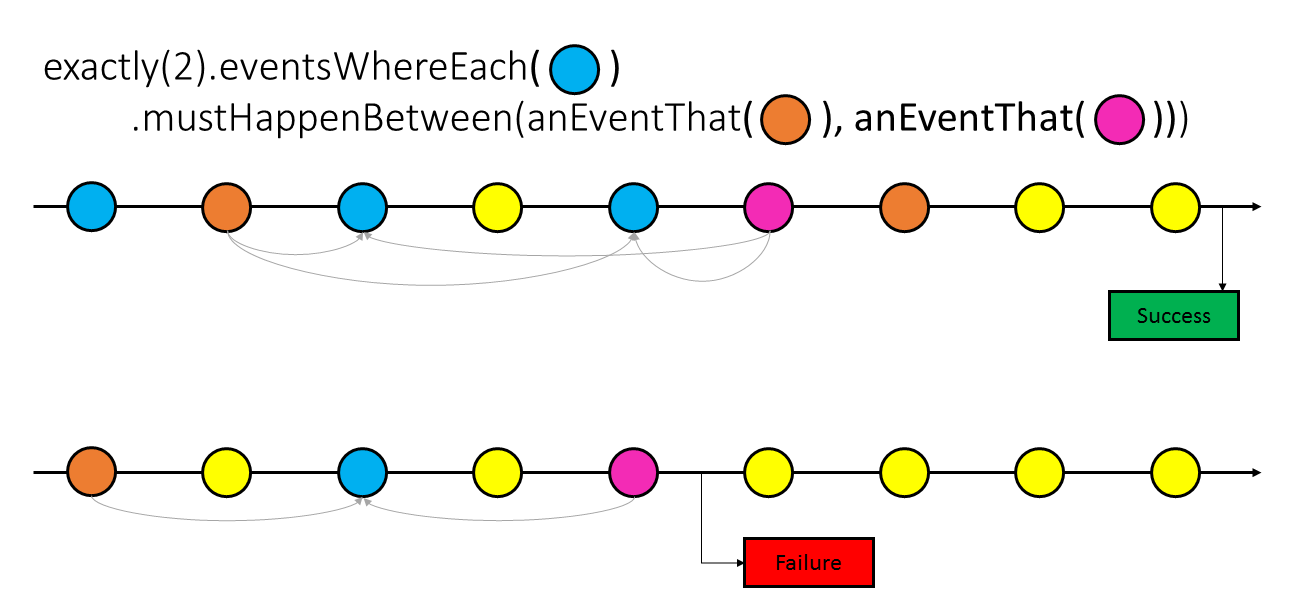
\includegraphics[width=400px]{Images/Event/Lang/Slide6.PNG}}
	
	
  	\\ \hline
  	
  \rotatebox[origin=c]{90}{\textbf{ Code Example }} & 
  
  	\begin{lstlisting}
	/* During the execution of the activity the text is changed exactly four times */
	exactly(4).eventsWhereEach(isTextChangeFrom(myTextView))
		.mustHappenBetween(
			anEventThat(isActivityLifecycleEvent(ON_RESUME)),
			anEventThat(isActivityLifecycleEvent(ON_PAUSE)));
	\end{lstlisting}
	
  	\\ \hline  	
  	 
\end{longtable}
\egroup
\end{center}


\subsection{Checks on the Whole Stream}

The third type of checks concerns the entire stream of events: they allow for example to specify the number of all the events of a certain type in the whole sequence generated by a particular execution.

\subsubsection{Match In Order}

\begin{center}
\bgroup
\def\arraystretch{1.5}%
\begin{longtable}{ | m{0.3cm} | m{15cm} | }
  \hline
  
  \rotatebox[origin=c]{90}{\textbf{ Structure }} & 
  
  	\begin{lstlisting}[mathescape]
	allEventsWhereEach(m).matchInOrder(m$_1$, m$_2$, ... , m$_n$)
	\end{lstlisting}
	
  	\\ \hline
  	 
  \rotatebox[origin=c]{90}{\textbf{ Description }} & 
  
  	Checks that \textit{all} the events that match \texttt{m} match in order the given matchers.
	
  	\\ \hline

  \rotatebox[origin=c]{90}{\textbf{ FOL }} & 
  
  	\begin{multline*}
	\forall e \bigg( match(e, m) \Rightarrow \exists i \Big( indexOf(e, m, i) \land match(e, m_i) \Big) \bigg)\\\\
indexOf(e, m, i) \equiv \exists_{=i} e' \Big( match(e', m) \land before(e', e) \Big)
	\end{multline*}
	
  	\\ \hline

  \rotatebox[origin=c]{90}{\textbf{ Visual }} & 
  
	\raisebox{-230pt}{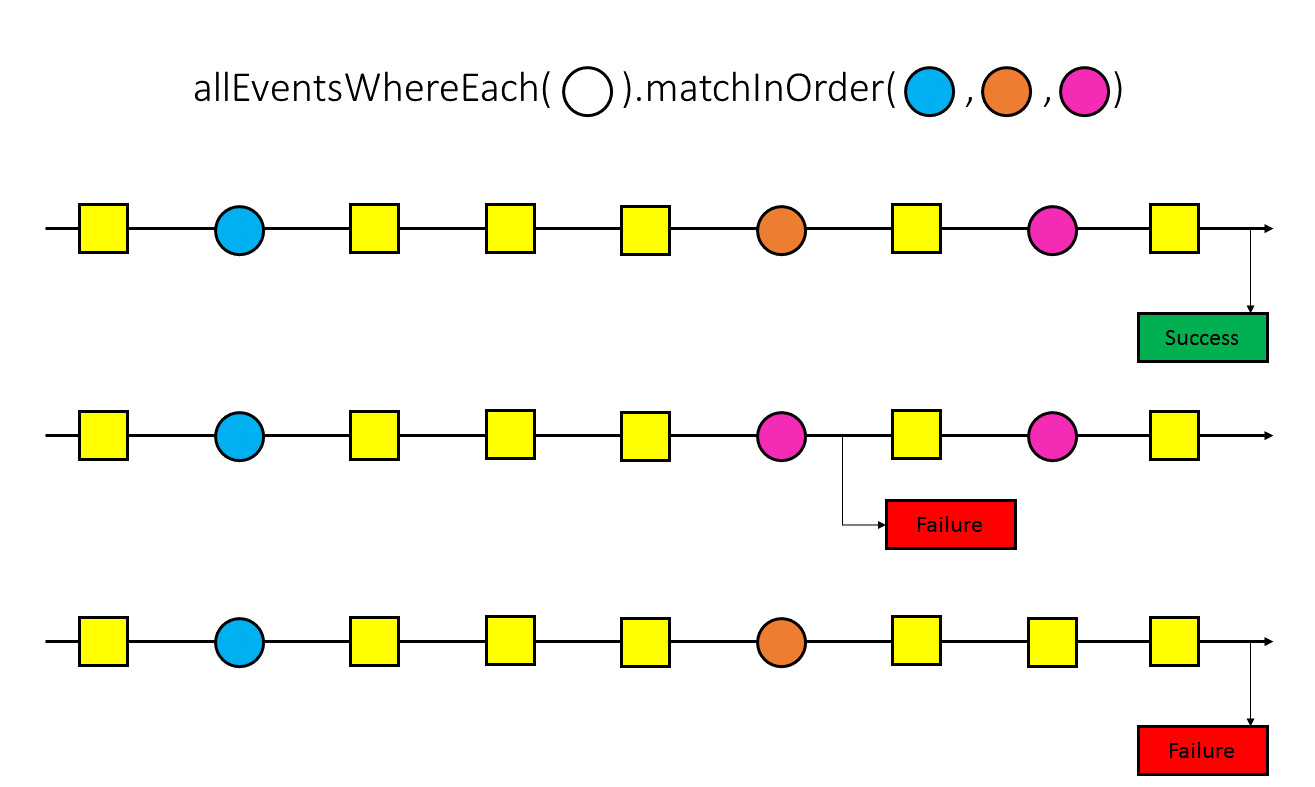
\includegraphics[width=400px]{Images/Event/Lang/Slide7.PNG}}
	
	Note in particular the last case: the check implicitly states that the events must be exactly 3 and they must satisfy the three matchers.	If the third one is missing, the check fails.
	
  	\\ \hline
  	
  \rotatebox[origin=c]{90}{\textbf{ Code Example }} & 
  
  	\begin{lstlisting}
	/* Defines the only valid fragment backstack changes sequence */	
	allEventsWhereEach(isFragmentBackstackChange())
		.matchInOrder(
			isFragmentBackstackPush(mainFragment),
			isFragmentBackstackPush(languageFragment),
			isFragmentBackstackPush(gameFragment),
			isFragmentBackstackPop(mainFragment));
	\end{lstlisting}
	
  	\\ \hline  	
  	 
\end{longtable}
\egroup
\end{center}

\subsubsection{Are Ordered}

\begin{center}
\bgroup
\def\arraystretch{1.5}%
\begin{longtable}{ | m{0.3cm} | m{15cm} | }
  \hline
  
  \rotatebox[origin=c]{90}{\textbf{ Structure }} & 
  
  	\begin{lstlisting}
	allEventsWhereEach(m).areOrdered(f)
	\end{lstlisting}
	
  	\\ \hline
  	 
  \rotatebox[origin=c]{90}{\textbf{ Description }} & 
  
  	Checks that \textit{all} the events that match \texttt{m} are in the order defined by the comparator function \textit{f} (receives two events and returns an integer $<$ 0 if the first is less than the second, 0 if they are equal, and $>$ 0 if the first is greater than the second).
	
  	\\ \hline

  \rotatebox[origin=c]{90}{\textbf{ FOL }} & 
  
  	\begin{multline*}
	\forall e, e' \bigg( match(e, m) \land match(e', m) \land before(e, e') \land\\ \neg \exists e'' \Big( match(e'', m) \land between(e, e'', e') \Big) \Rightarrow ordered(f, e, e') \bigg)\\\\
ordered(com, e1, e2) \equiv \bigg( \Big( com<0 \Rightarrow before(e1, e2) \Big) \lor\\ \Big( com=0 \Rightarrow before(e1, e2) \lor before(e2, e1) \Big) \lor\\ \Big( com>0 \Rightarrow before(e2, e1) \Big) \bigg)
	\end{multline*}
	
  	\\ \hline

  \rotatebox[origin=c]{90}{\textbf{ Visual }} & 
  
	\raisebox{-160pt}{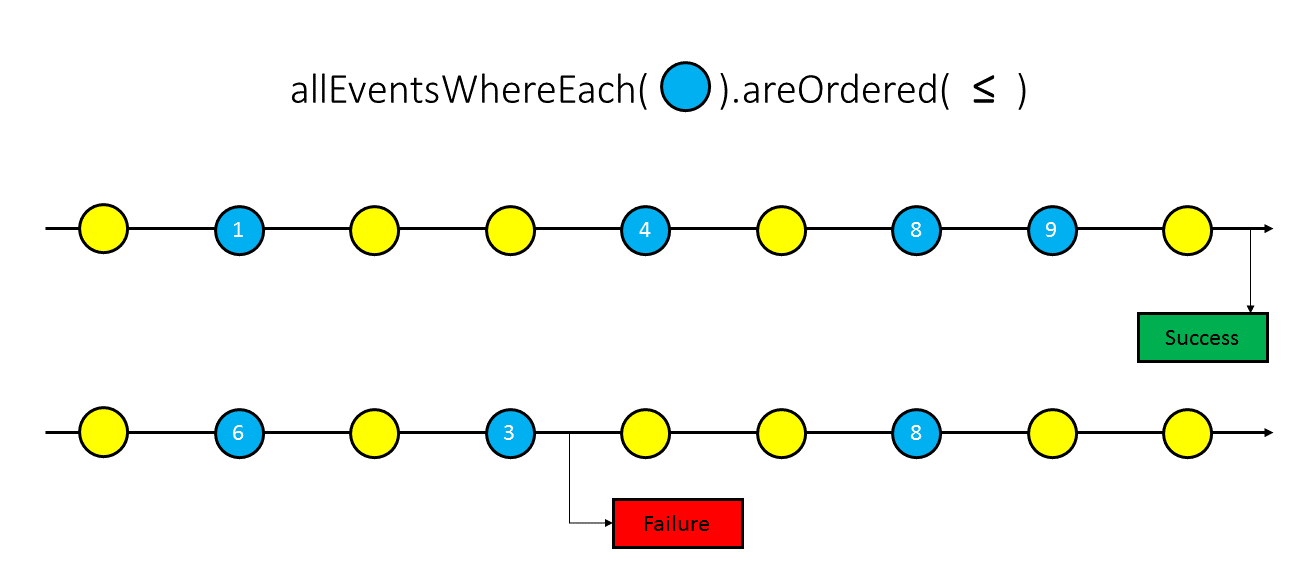
\includegraphics[width=400px]{Images/Event/Lang/Slide8.PNG}}
	
	
  	\\ \hline
  	
  \rotatebox[origin=c]{90}{\textbf{ Code Example }} & 
  
  	\begin{lstlisting}
	/* The text in the countdown is updated in the correct (inverse) order */
	allEventsWhereEach(isTextChangeFrom(countdownView))
		.areOrdered(new Comparator<TextChangeEvent>()
					{
						@Override
						public int compare(TextChangeEvent lhs, TextChangeEvent rhs)
						{
							String t1 = lhs.getText();
							String t2 = rhs.getText();
							return Integer.compare(Integer.valueOf(t2),
												   Integer.valueOf(t1));
						}
					}));
	\end{lstlisting}
	
  	\\ \hline  	
  	 
\end{longtable}
\egroup
\end{center}

\subsection{Existential Checks}

These checks assess the existence of one or more events in the stream. Similarly to the previous categories, only the formulas for "exactly" will be formalized.

\subsubsection{Exists An Event}

\begin{center}
\bgroup
\def\arraystretch{1.5}%
\begin{longtable}{ | m{0.3cm} | m{15cm} | }
  \hline
  
  \rotatebox[origin=c]{90}{\textbf{ Structure }} & 
  
  	\begin{lstlisting}
	existsAnEventThat(m)
	\end{lstlisting}
	
  	\\ \hline
  	 
  \rotatebox[origin=c]{90}{\textbf{ Description }} & 
  
  	Checks that at least one event that matches the matcher \texttt{m} exists anywhere in the sequence.
	
  	\\ \hline

  \rotatebox[origin=c]{90}{\textbf{ FOL }} & 
  
  	\begin{multline*}
	\exists e \Big( match(e, m) \Big)
	\end{multline*}
	
  	\\ \hline

  \rotatebox[origin=c]{90}{\textbf{ Visual }} & 
  
	\raisebox{-170pt}{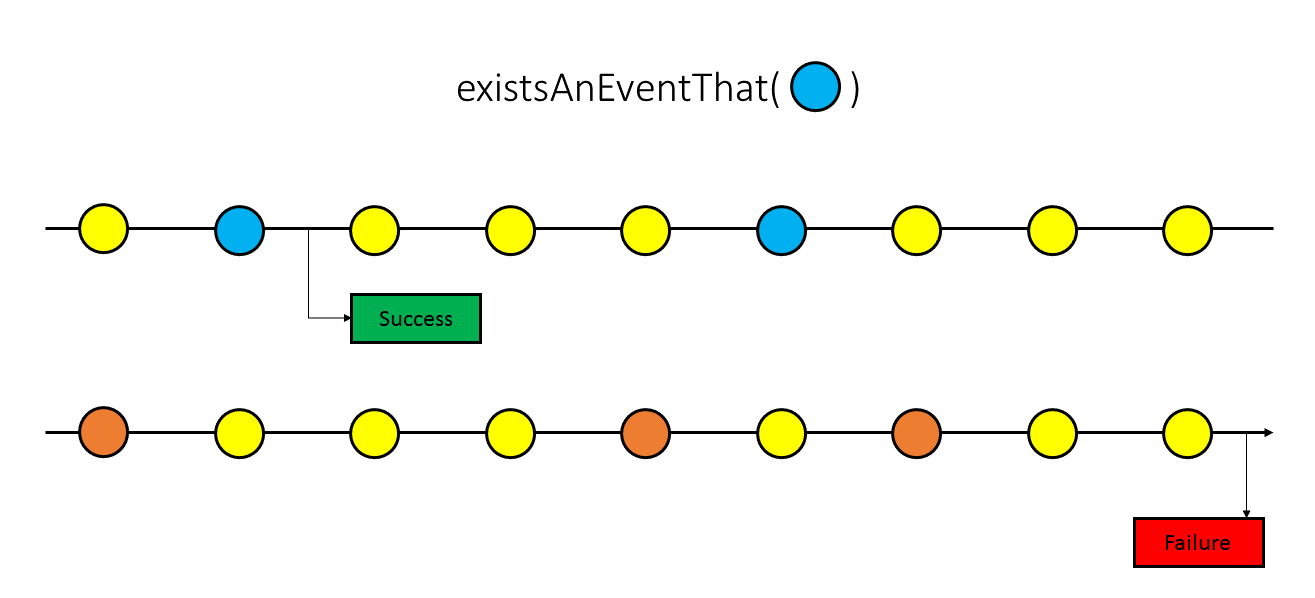
\includegraphics[width=400px]{Images/Event/Lang/Slide9.PNG}}
	
	
  	\\ \hline
  	
  \rotatebox[origin=c]{90}{\textbf{ Code Example }} & 
  
  	\begin{lstlisting}
	/* The database must be opened sooner or later during the execution */
	existsAnEventThat(isOpenDatabase());
	\end{lstlisting}
	
  	\\ \hline  	
  	 
\end{longtable}
\egroup
\end{center}

\subsubsection{Exist Events}

\begin{center}
\bgroup
\def\arraystretch{1.5}%
\begin{longtable}{ | m{0.3cm} | m{15cm} | }
  \hline
  
  \rotatebox[origin=c]{90}{\textbf{ Structure }} & 
  
  	\begin{lstlisting}
	exist(exactly(n)).eventsWhereEach(m)
	\end{lstlisting}
	
  	\\ \hline
  	 
  \rotatebox[origin=c]{90}{\textbf{ Description }} & 
  
  	Checks that the events that match \texttt{m} are exactly \texttt{n} in the whole stream.
	
  	\\ \hline

  \rotatebox[origin=c]{90}{\textbf{ FOL }} & 
  
  	\begin{multline*}
	\exists_{=n} e \Big( match(e, m) \Big)
	\end{multline*}
	
  	\\ \hline

  \rotatebox[origin=c]{90}{\textbf{ Visual }} & 
  
	\raisebox{-170pt}{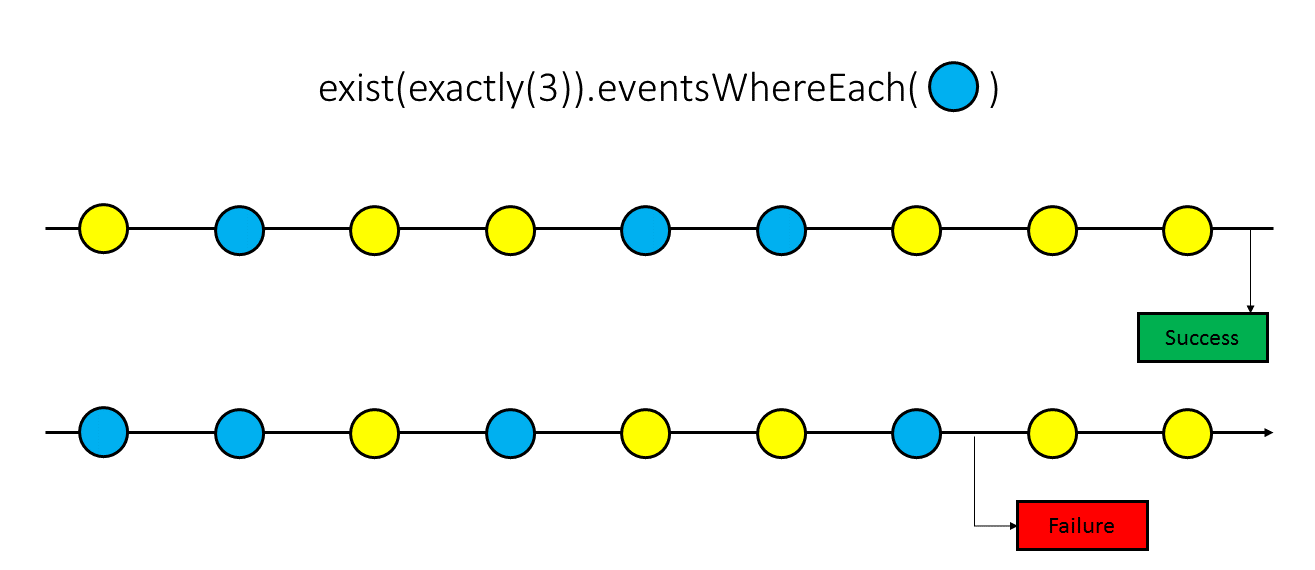
\includegraphics[width=400px]{Images/Event/Lang/Slide10.PNG}}
	
	
  	\\ \hline
  	
  \rotatebox[origin=c]{90}{\textbf{ Code Example }} & 
  
  	\begin{lstlisting}
	/* In this execution the system sends exactly 10 broadcasts */
	exist(exactly(10))
		.eventsWhereEach(isSendBroadcast());
	\end{lstlisting}
	
  	\\ \hline  	
  	 
\end{longtable}
\egroup
\end{center}

\fxnote*{New}{
\subsubsection{Exist Events After}}

\begin{center}
\bgroup
\def\arraystretch{1.5}%
\begin{longtable}{ | m{0.3cm} | m{15cm} | }
  \hline
  
  \rotatebox[origin=c]{90}{\textbf{ Structure }} & 
  
  	\begin{lstlisting}
	exist(after(anEventThat(m2)), exactly(n)).eventsWhereEach(m1)
	\end{lstlisting}
	
  	\\ \hline
  	 
  \rotatebox[origin=c]{90}{\textbf{ Description }} & 
  
  	Similar to the unbounded existential quantifier described in the previous section but with a restriction on the validity interval: exactly \texttt{n} events that match \texttt{m1} must exist exclusively after \textit{an} event (i.e. at least once) that matches \texttt{m2}.
	
  	\\ \hline

  \rotatebox[origin=c]{90}{\textbf{ FOL }} & 
  
  	\begin{multline*}
	\exists_{=n} e1 \Bigg( match(e1, m1) \land \bigg( \exists e2 \Big( match(e2, m2) \land before(e2, e1) \land \\ \neg \exists e2' \big( match(e2', m2) \land between(e2, e2', e1) \big) \Big) \bigg) \Bigg)
	\end{multline*}
	
  	\\ \hline

  \rotatebox[origin=c]{90}{\textbf{ Visual }} & 
  
	\raisebox{-200pt}{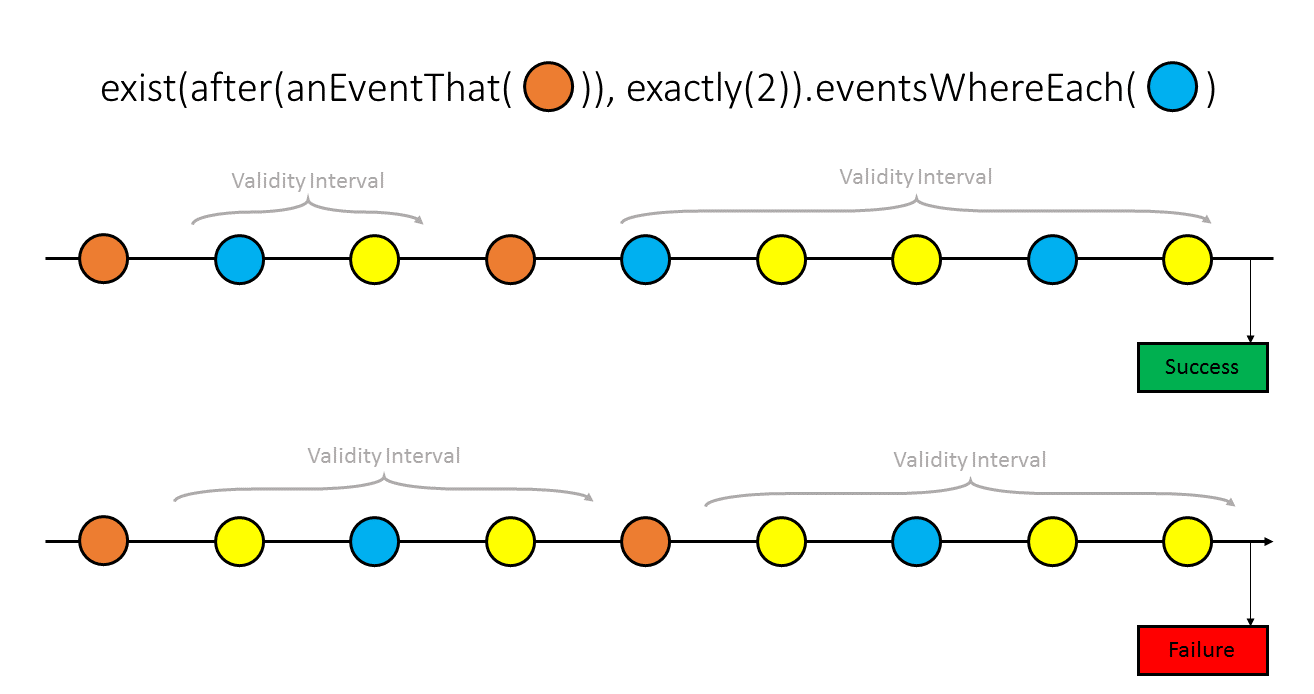
\includegraphics[width=400px]{Images/Event/Lang/Slide16.PNG}}
	
	
  	\\ \hline
  	
  \rotatebox[origin=c]{90}{\textbf{ Code Example }} & 
  
  	\begin{lstlisting}
	/* At least one click must be followed by a broadcast */
	exist(
		after(anEventThat(isClickOn(myButton))),
		exactly(1))
			.eventsWhereEach(isSendBroadcast());
	\end{lstlisting}
	
  	\\ \hline  	
  	 
\end{longtable}
\egroup
\end{center}

\fxnote*{New}{
\subsubsection{Exist Events Before}}

\begin{center}
\bgroup
\def\arraystretch{1.5}%
\begin{longtable}{ | m{0.3cm} | m{15cm} | }
  \hline
  
  \rotatebox[origin=c]{90}{\textbf{ Structure }} & 
  
  	\begin{lstlisting}
	exist(before(anEventThat(m2)), exactly(n)).eventsWhereEach(m1)
	\end{lstlisting}
	
  	\\ \hline
  	 
  \rotatebox[origin=c]{90}{\textbf{ Description }} & 
  
  	Similar to the unbounded existential quantifier but with a restriction on the validity interval: exactly \texttt{n} events that match \texttt{m1} must exist exclusively before \textit{an} event (i.e. at least once) that matches \texttt{m2}.
	
  	\\ \hline

  \rotatebox[origin=c]{90}{\textbf{ FOL }} & 
  
  	\begin{multline*}
	\exists_{=n} e1 \Bigg( match(e1, m1) \land \bigg( \exists e2 \Big( match(e2, m2) \land before(e1, e2) \land \\ \neg \exists e2' \big( match(e2', m2) \land between(e1, e2', e2) \big) \Big) \bigg) \Bigg)
	\end{multline*}
	
  	\\ \hline

  \rotatebox[origin=c]{90}{\textbf{ Visual }} & 
  
	\raisebox{-200pt}{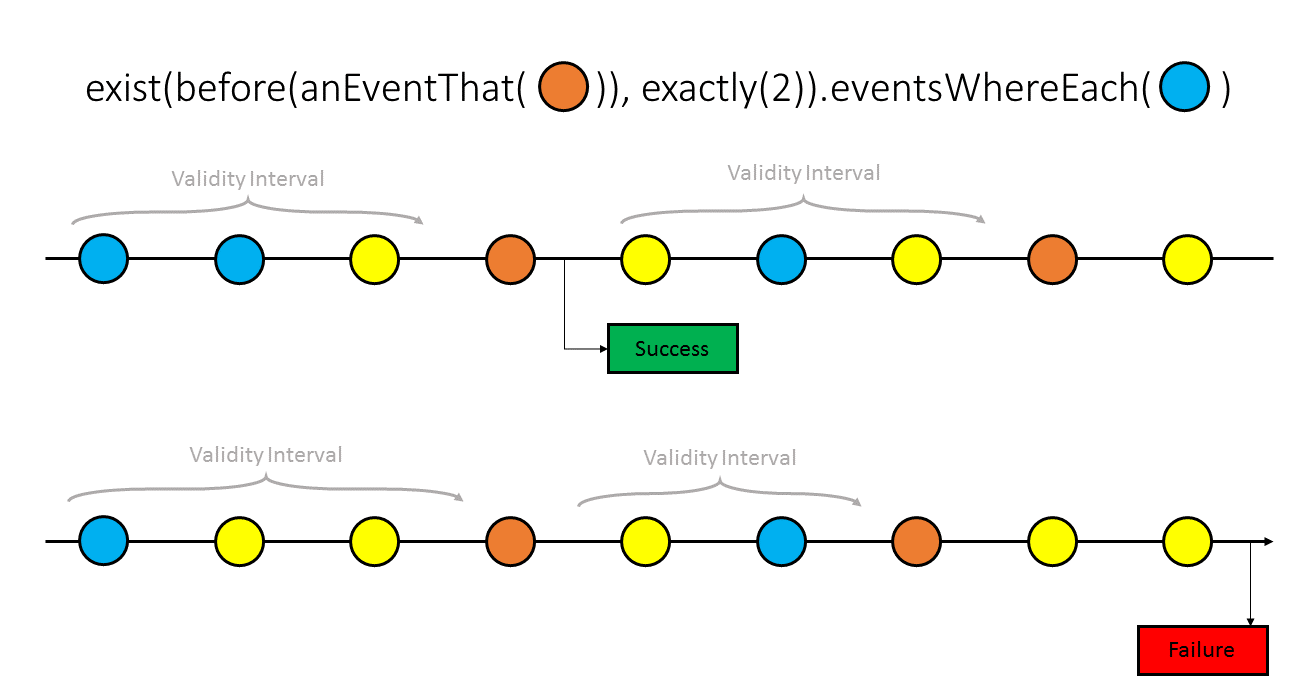
\includegraphics[width=400px]{Images/Event/Lang/Slide17.PNG}}
	
	
  	\\ \hline
  	
  \rotatebox[origin=c]{90}{\textbf{ Code Example }} & 
  
  	\begin{lstlisting}
	/* At least once, the service starts after a fragment initialization */
	exist(
		before(anEventThat(isServiceStart(mainService))),
		exactly(1))
			.eventsWhereEach(isFragmentLifecycleEvent(ON_CREATE));
	\end{lstlisting}
	
  	\\ \hline  	
  	 
\end{longtable}
\egroup
\end{center}

\fxnote*{New}{
\subsubsection{Exist Events Between}}

\begin{center}
\bgroup
\def\arraystretch{1.5}%
\begin{longtable}{ | m{0.3cm} | m{15cm} | }
  \hline
  
  \rotatebox[origin=c]{90}{\textbf{ Structure }} & 
  
  	\begin{lstlisting}
	exist(between(anEventThat(m2), anEventThat(m3)), exactly(n)).eventsWhereEach(m1)
	\end{lstlisting}
	
  	\\ \hline
  	 
  \rotatebox[origin=c]{90}{\textbf{ Description }} & 
  
  	Similar to the unbounded existential quantifier but with a restriction on the validity interval: exactly \texttt{n} events that match \texttt{m1} must exist exclusively between \textit{a} pair (i.e. at least once) of events where the first matches \texttt{m2} and the second matches \texttt{m3}.
	
  	\\ \hline

  \rotatebox[origin=c]{90}{\textbf{ FOL }} & 
  
  	\begin{multline*}
	\exists_{=n} e1 \Bigg( match(e1, m1) \land \bigg( \exists e2, e3 \Big( match(e2, m2) \land match(e3, m3) \land \\ between(e2, e1, e3) \land \neg \exists e2', e3' \big( match(e2', m2) \land between(e2, e2', e3) \lor \\ match(e3', m3) \land between(e2, e3', e3) \big) \Big) \bigg) \Bigg)
	\end{multline*}
	
  	\\ \hline

  \rotatebox[origin=c]{90}{\textbf{ Visual }} & 
  
	\raisebox{-200pt}{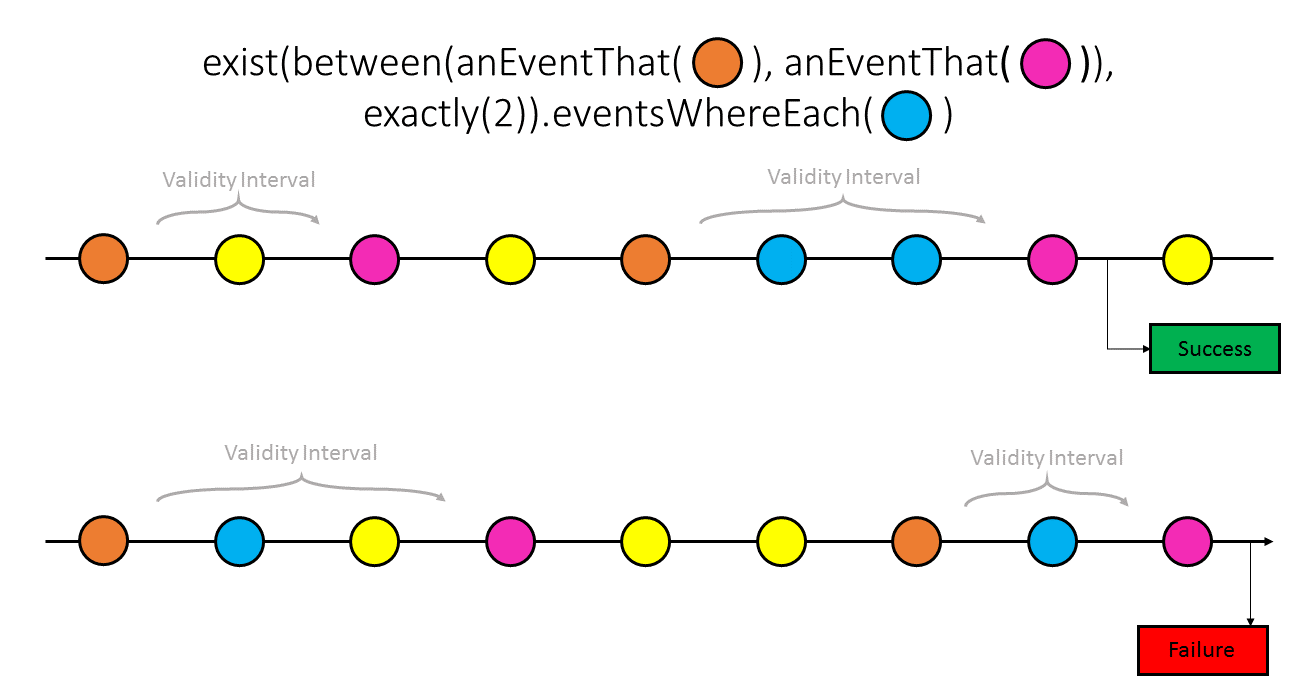
\includegraphics[width=400px]{Images/Event/Lang/Slide18.PNG}}
	
	
  	\\ \hline
  	
  \rotatebox[origin=c]{90}{\textbf{ Code Example }} & 
  
  	\begin{lstlisting}
	/* At least once, the service must query the database during its execution */
	exist(
		between(anEventThat(isServiceStart(mainService)),
				anEventThat(isServiceStart(mainService))),
		exactly(3))
			.eventsWhereEach(isDatabaseQuery());
	\end{lstlisting}
	
  	\\ \hline  	
  	 
\end{longtable}
\egroup
\end{center}


\subsection{Connectives between Checks}

These constructs allow to specify the standard logic connectives between one or more of the previously defined consistency checks.

\subsubsection{And}

\begin{center}
\bgroup
\def\arraystretch{1.5}%
\begin{longtable}{ | m{0.3cm} | m{15cm} | }
  \hline
  
  \rotatebox[origin=c]{90}{\textbf{ Structure }} & 
  
  	\begin{lstlisting}
	allHold(c1, c2,...)
	\end{lstlisting}
	
  	\\ \hline
  	 
  \rotatebox[origin=c]{90}{\textbf{ Description }} & 
  
  	All sub-checks \textit{c1}, \textit{c2}, etc. must succeed.
	
  	\\ \hline

  \rotatebox[origin=c]{90}{\textbf{ FOL }} & 
  
  	\begin{multline*}
	c1 \land c2 \land ...
	\end{multline*}
	
  	\\ \hline

  \rotatebox[origin=c]{90}{\textbf{ Visual }} & 
  
	\raisebox{-105pt}{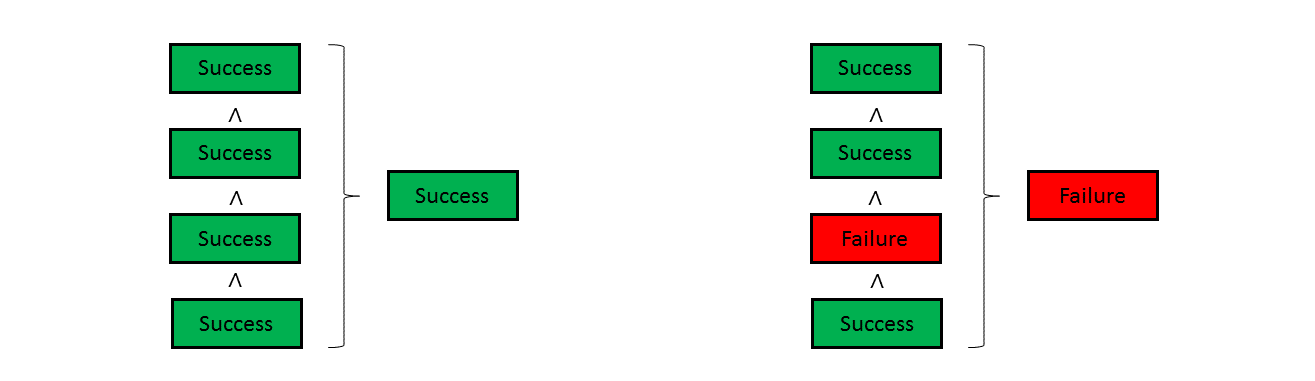
\includegraphics[width=400px]{Images/Event/Lang/Slide11.png}}
	
	
  	\\ \hline
  	
  \rotatebox[origin=c]{90}{\textbf{ Code Example }} & 
  
  	\begin{lstlisting}
	/* The service must only be started after the button is clicked */
	allHold(
		anEventThat(isStartService())
			.canHappenOnlyAfter(isClickOn(startButton)),
		exactly(1).eventsWhereEach(isStartService())
			.mustHappenAfter(isClickOn(startButton)));
	\end{lstlisting}
	
  	\\ \hline  	
  	 
\end{longtable}
\egroup
\end{center}

\subsubsection{Or}

\begin{center}
\bgroup
\def\arraystretch{1.5}%
\begin{longtable}{ | m{0.3cm} | m{15cm} | }
  \hline
  
  \rotatebox[origin=c]{90}{\textbf{ Structure }} & 
  
  	\begin{lstlisting}
	anyHolds(c1, c2,...)
	\end{lstlisting}
	
  	\\ \hline
  	 
  \rotatebox[origin=c]{90}{\textbf{ Description }} & 
  
  	At least one sub-check must succeed.
	
  	\\ \hline

  \rotatebox[origin=c]{90}{\textbf{ FOL }} & 
  
  	\begin{multline*}
	c1 \lor c2 \lor ...
	\end{multline*}
	
  	\\ \hline

  \rotatebox[origin=c]{90}{\textbf{ Visual }} & 
  
	\raisebox{-105pt}{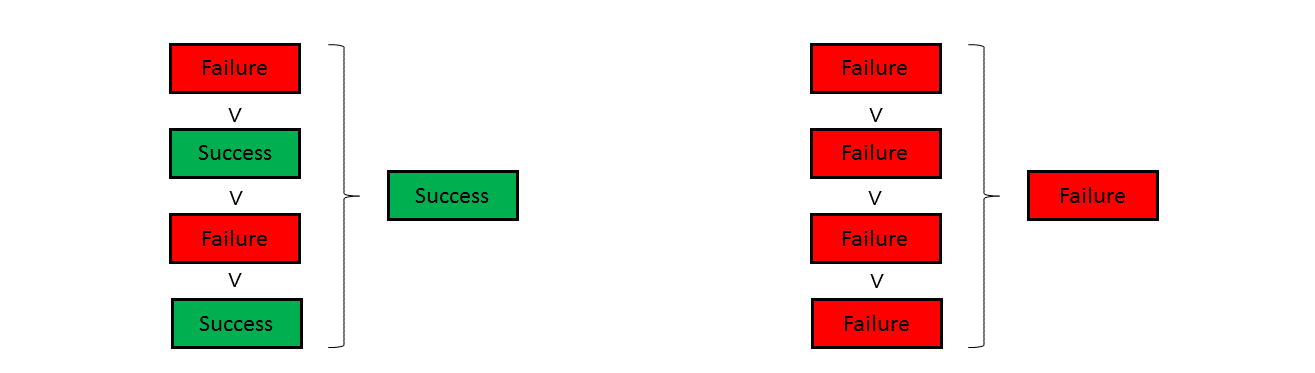
\includegraphics[width=400px]{Images/Event/Lang/Slide12.PNG}}
	
	
  	\\ \hline
  	
  \rotatebox[origin=c]{90}{\textbf{ Code Example }} & 
  
  	\begin{lstlisting}
	/* Either succeed or fail download (no situations where the user is not notified) */		
	anyHolds(
		exist(exactly(1))
			.eventsWhereEach(isDownloadSuccess()),
		exist(exactly(1))
			.eventsWhereEach(isDownloadError()));
	\end{lstlisting}
	
  	\\ \hline  	
  	 
\end{longtable}
\egroup
\end{center}

\subsubsection{Not}

\begin{center}
\bgroup
\def\arraystretch{1.5}%
\begin{longtable}{ | m{0.3cm} | m{15cm} | }
  \hline
  
  \rotatebox[origin=c]{90}{\textbf{ Structure }} & 
  
  	\begin{lstlisting}
	isNotSatisfied(c)
	\end{lstlisting}
	
  	\\ \hline
  	 
  \rotatebox[origin=c]{90}{\textbf{ Description }} & 
  
  	Inverts the outcome of the sub-check.
	
  	\\ \hline

  \rotatebox[origin=c]{90}{\textbf{ FOL }} & 
  
  	\begin{multline*}
	\neg c
	\end{multline*}
	
  	\\ \hline

  \rotatebox[origin=c]{90}{\textbf{ Visual }} & 
  
	\raisebox{-70pt}{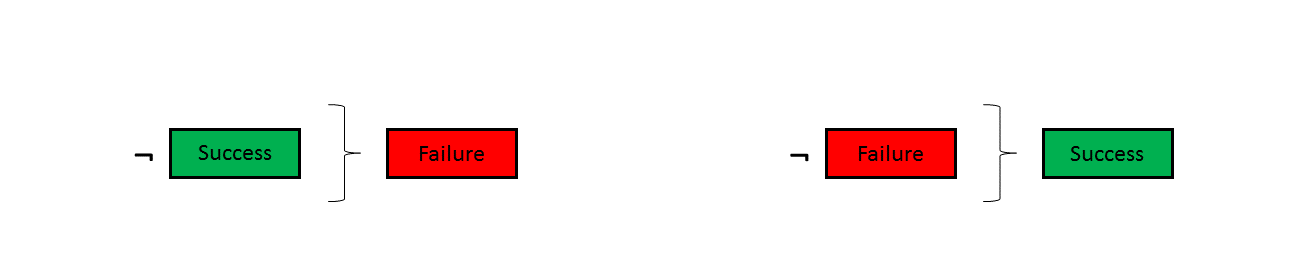
\includegraphics[width=400px]{Images/Event/Lang/Slide13.PNG}}
	
	
  	\\ \hline
  	
  \rotatebox[origin=c]{90}{\textbf{ Code Example }} & 
  
  	\begin{lstlisting}
	/* In this execution the email draft cannot be saved */		
	isNotSatisfied(
		existsAnEventThat(isSaveDraft()));
	\end{lstlisting}
	
  	\\ \hline  	
  	 
\end{longtable}
\egroup
\end{center}

\subsubsection{Single Implication}

\begin{center}
\bgroup
\def\arraystretch{1.5}%
\begin{longtable}{ | m{0.3cm} | m{15cm} | }
  \hline
  
  \rotatebox[origin=c]{90}{\textbf{ Structure }} & 
  
  	\begin{lstlisting}
	providedThat(c1).then(c2)
	\end{lstlisting}
	
  	\\ \hline
  	 
  \rotatebox[origin=c]{90}{\textbf{ Description }} & 
  
  	\texttt{c2} is checked only if \texttt{c1} succeeds.
	
  	\\ \hline

  \rotatebox[origin=c]{90}{\textbf{ FOL }} & 
  
  	\begin{multline*}
	c1 \Rightarrow c2
	\end{multline*}
	
  	\\ \hline

  \rotatebox[origin=c]{90}{\textbf{ Visual }} & 
  
	\raisebox{-140pt}{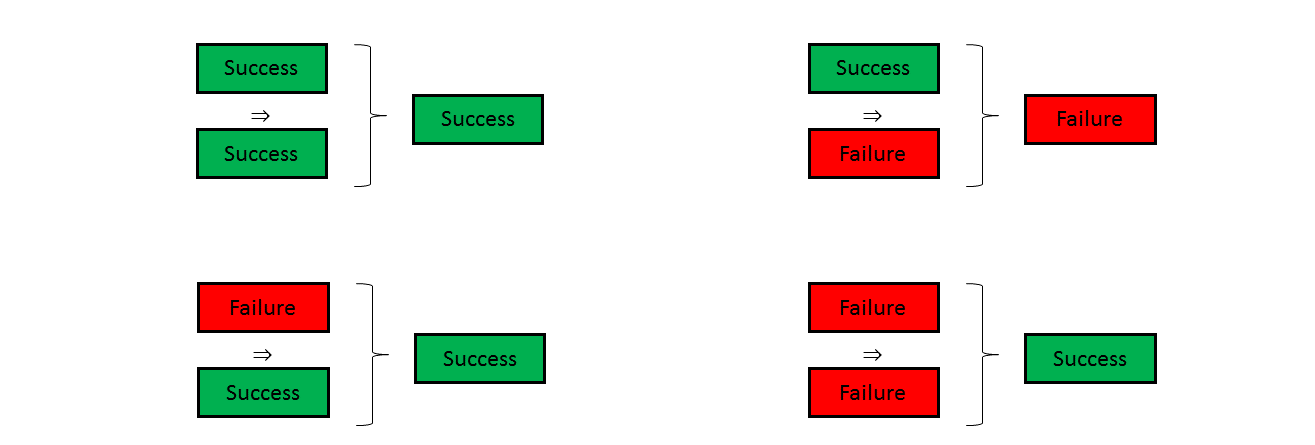
\includegraphics[width=400px]{Images/Event/Lang/Slide14.PNG}}
	
	
  	\\ \hline
  	
  \rotatebox[origin=c]{90}{\textbf{ Code Example }} & 
  
  	\begin{lstlisting}
	/* If the list order changes, then we must update the database */
	providedThat(
			exist(atLeast(1))
				.eventsWhereEach(isListOrderChange()))
		.then(
			exist(exactly(1))
				.eventsWhereEach(isSaveDatabase()));
	\end{lstlisting}
	
  	\\ \hline  	
  	 
\end{longtable}
\egroup
\end{center}

\subsubsection{Double Implication}

\begin{center}
\bgroup
\def\arraystretch{1.5}%
\begin{longtable}{ | m{0.3cm} | m{15cm} | }
  \hline
  
  \rotatebox[origin=c]{90}{\textbf{ Structure }} & 
  
  	\begin{lstlisting}
	isSatisfied(c1).iff(c2)
	\end{lstlisting}
	
  	\\ \hline
  	 
  \rotatebox[origin=c]{90}{\textbf{ Description }} & 
  
  	Succeeds only if both sub-checks fail or both succeed.
	
  	\\ \hline

  \rotatebox[origin=c]{90}{\textbf{ FOL }} & 
  
  	\begin{multline*}
	c1 \iff c2
	\end{multline*}
	
  	\\ \hline

  \rotatebox[origin=c]{90}{\textbf{ Visual }} & 
  
	\raisebox{-140pt}{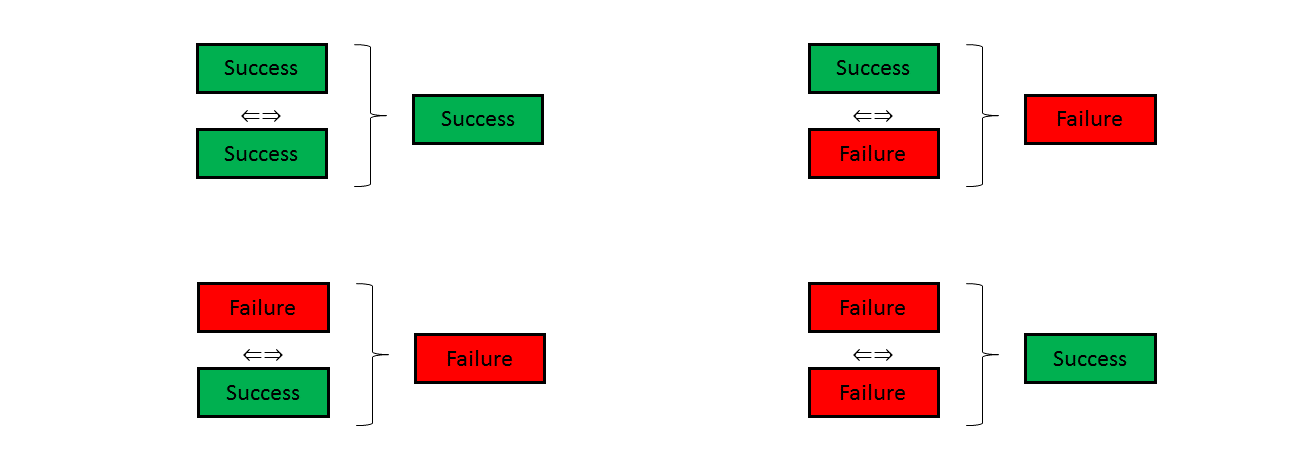
\includegraphics[width=400px]{Images/Event/Lang/Slide15.PNG}}
	
	
  	\\ \hline
  	
  \rotatebox[origin=c]{90}{\textbf{ Code Example }} & 
  
  	\begin{lstlisting}
	/* Send email if and only if the user clicks on the send button */			
	isSatisfied(
			existsAnEventThat(isClickOn(sendButton)))
		.iff(
			existsAnEventThat(isSendEmail()));
	\end{lstlisting}
	
  	\\ \hline  	
  	 
\end{longtable}
\egroup
\end{center}

\section{Design}\label{event_design}
To implement the event-based testing approach described so far, the following main components are employed:
\begin{itemize}
	\item Events: objects that represent events in the application.
	\item Event Generators: structures that actually create the events whenever something happens in the application.
	\item Checks: ways to specify the consistency rules defined in the previous section.
	\item Results: the outcomes of the checks.
	\item Event Monitor: the main interface of the system, receives the events, applies the checks and produces the results.
\end{itemize}
\begin{figure}\medskip
  \centering
  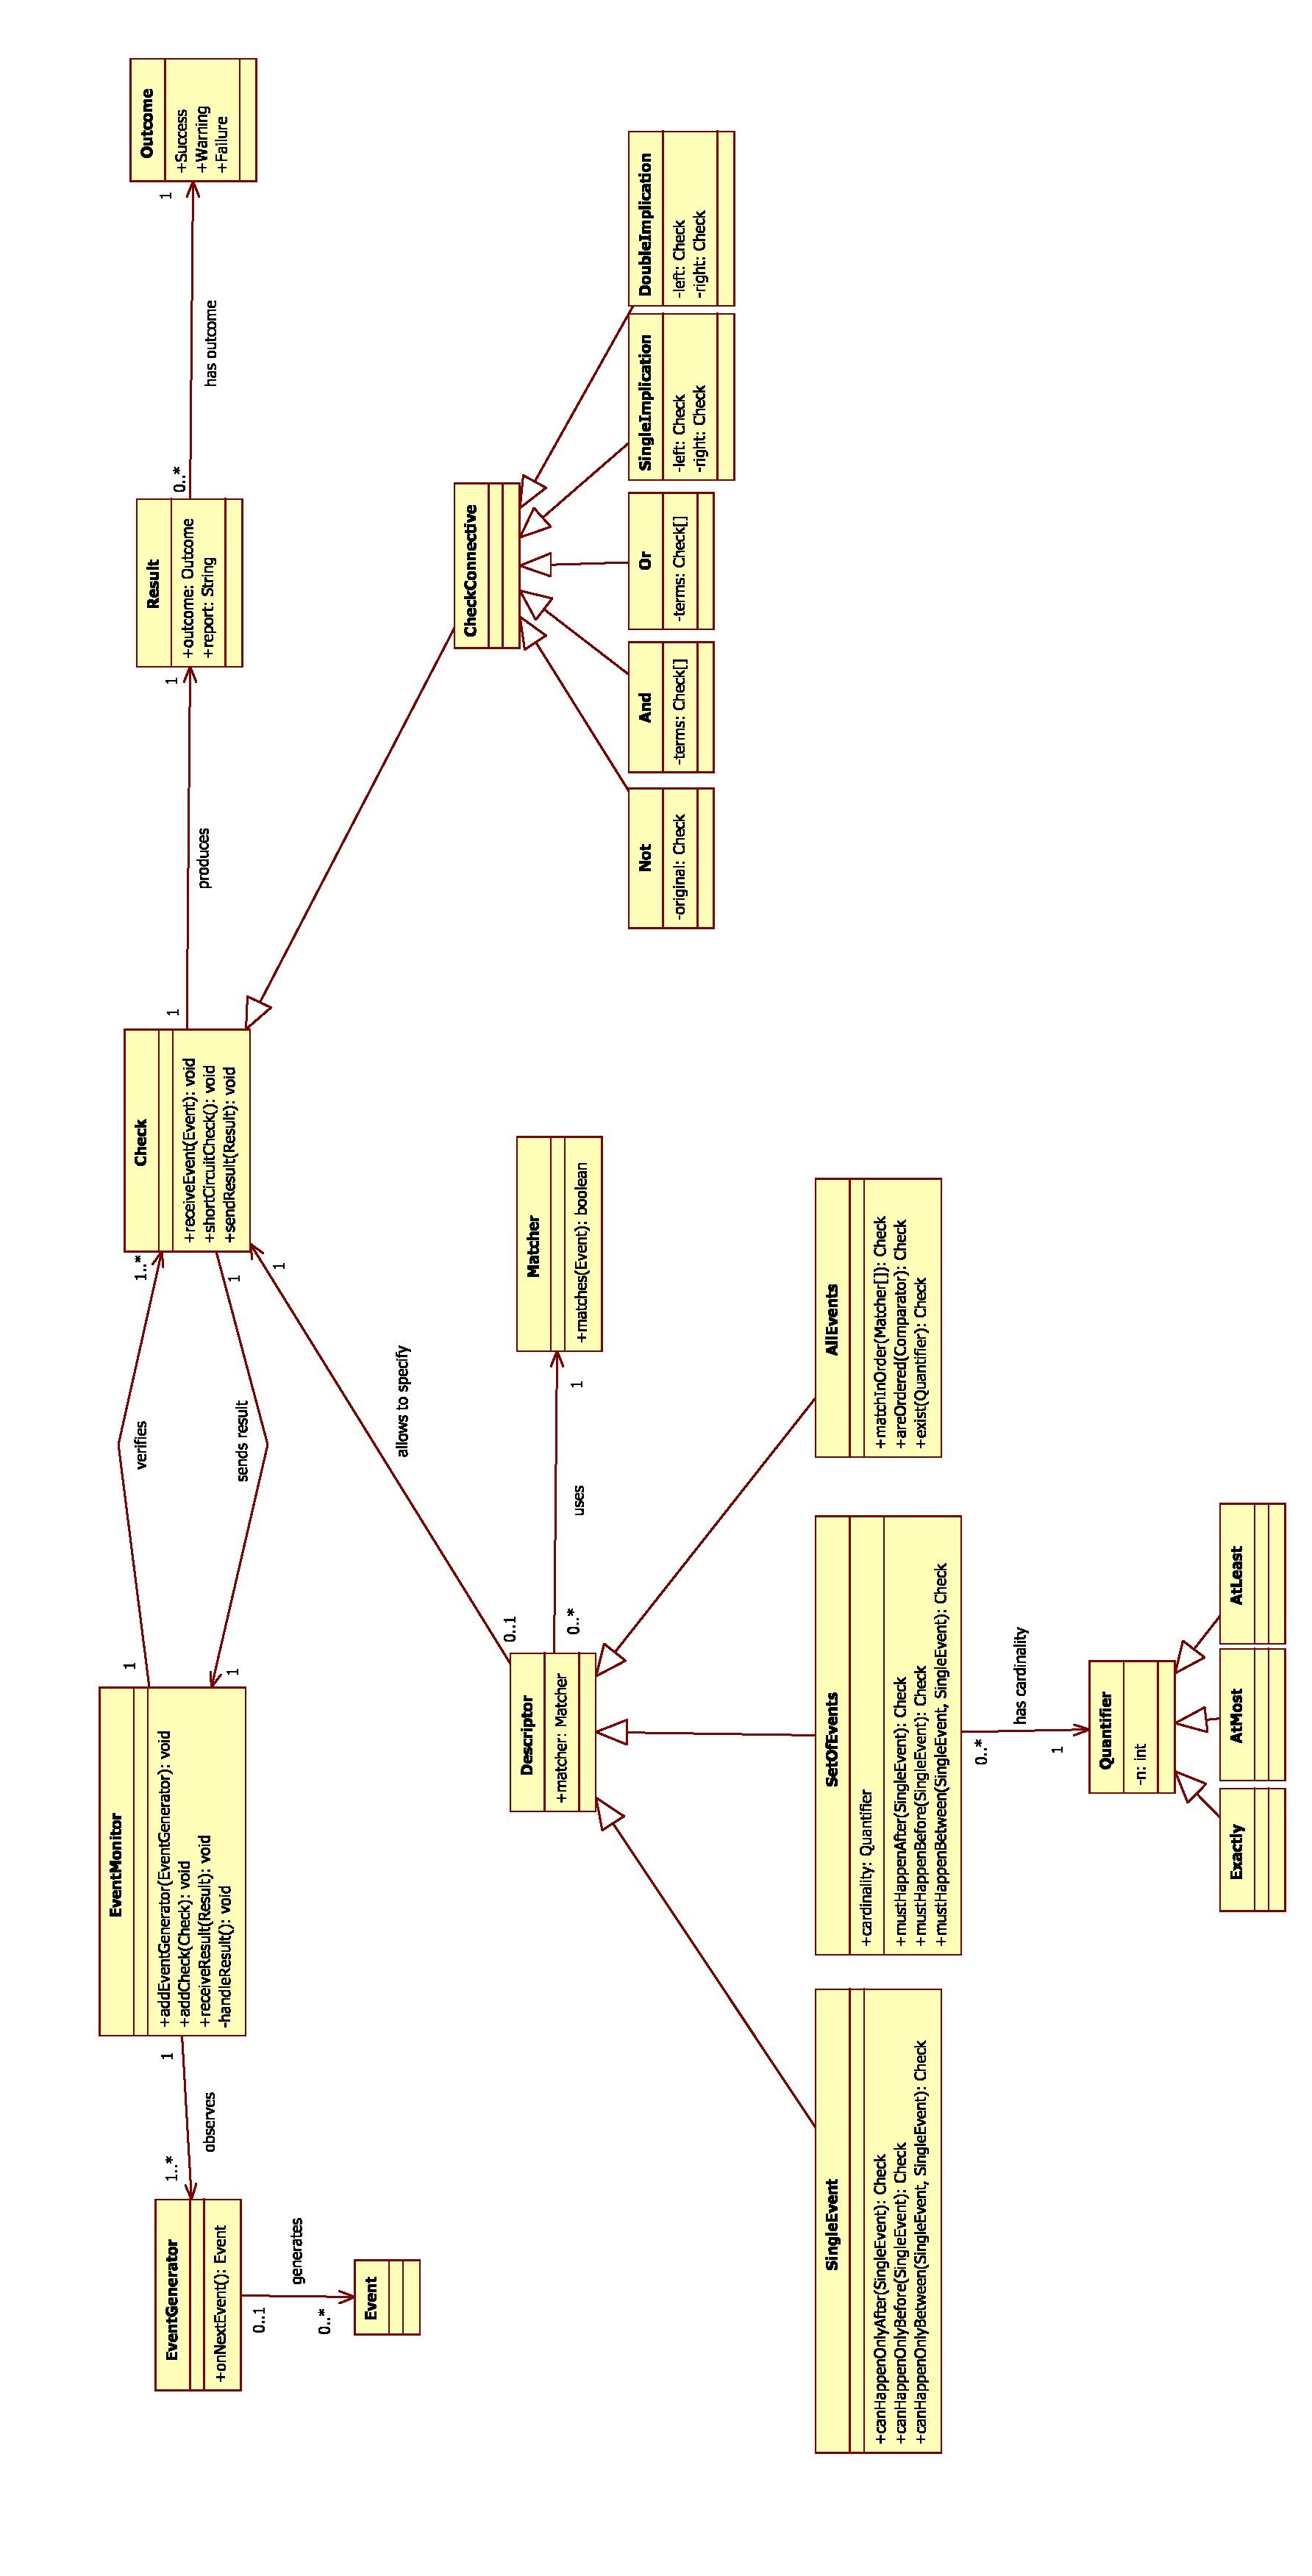
\includegraphics[height=\textheight]{Images/Event/UML/Design.jpg}
  \caption[Event-Based Testing Design UML]{UML Diagram for the Event-Based Testing Design}
  \label{fig:event_uml_design}
\end{figure}
Figure \ref{fig:event_uml_design} shows the design UML class diagram. The \textit{EventMonitor} offers methods to add one or more \textit{EventGenerator} objects to define the event stream, to add one or more \textit{Check} objects to be verified and handles the \textit{Result} objects in some way (e.g. makes a test case fail if the \textit{Result} is a failure).\medskip \\
Each \textit{Check} contains the logic of a consistency check: it receives each \textit{Event} of the stream in order and acts accordingly. A \textit{Check} has the possibility to short-circuit its behavior (i.e. interrupt the stream of events if the consistency check succeeds or fails before the end of the sequence). In any case, when it short-circuits or the stream comes to an end, the \textit{Check} produces one and only one \textit{Result} object.\medskip \\
Each \textit{Result} contains an \textit{Outcome} and a message describing it. In particular, an \textit{Outcome} can be a \textit{Success}, a \textit{Failure} and a \textit{Warning}. A \textit{Warning} outcome has not been included in the formal specifications of the checks in the previous section for simplicity: its meaning is that the \textit{Check} succeeded with some minor error or in a particular situation (for example a check that specifies that an event A always generates exactly one event B may return \textit{Warning} if no event A has been found in the sequence).\medskip \\
A \textit{Descriptor} allows to specify a \textit{Check}, i.e. it is the main component of the temporal assertion language syntax. It describes one or more events of the stream and provides methods to express a condition on them. In particular, \textit{SingleEvent} describes a single event of a certain type at a time, \textit{SetOfEvents} describes a set of events of a certain type at a time and \textit{AllEvents} describes all the events of a certain type in the whole stream. To determine the type of the events identified by the \textit{Descriptor}, a \textit{Matcher} object is used.\medskip \\
The cardinality of the descriptor \textit{SetOfEvents} is defined by a \textit{Quantifier} that has an integer value as input. A quantifier can be \textit{Exactly}, \textit{AtMost} or \textit{AtLeast}.\medskip \\
Finally, a \textit{CheckConnective} allows to transform one or more \textit{Check} objects into a single \textit{Check}, i.e. it specifies one of the standard logic connectives \textit{Not}, \textit{And}, \textit{Or}, \textit{SingleImplication} and \textit{DoubleImplication}.

\section{Implementation}

For the implementation of event-based testing~\cite{EventBasedTesting}, the ReactiveX library~\cite{ReactiveX} was chosen. This innovative reactive programming paradigm focuses on data flow: this means generating (statically or dynamically) and propagating a flow of events, allowing interested components to react to them. The idea of reactive programming is fire-and-forget messaging: send a request and asynchronously wait for the response to be ready or, even more importantly, in case of response sets wait for individual results to be forwarded (without waiting for the whole set to be computed).\bigskip \\
In the next sections a more detailed introduction to the ReactiveX library is presented, followed by the implementation of the proposed event-based testing testing tool.

\subsection{ReactiveX}
The Reactive Extensions (ReactiveX or Rx) are a reactive programming library to compose asynchronous and event-based programs. As defined by its authors, ReactiveX is a combination of the best ideas from:
\begin{itemize}
	\item The Observer pattern (design pattern where a subject automatically notifies the so-called observers of its state changes).
	\item The Iterator pattern (design pattern where an iterator is used to traverse a collection of elements, like an array).
	\item Functional Programming (declarative programming paradigm where computation is performed via mathematical functions that are not allowed to change the state of the system).
\end{itemize}
This approach is asynchronous because many instructions may execute in parallel and their results (events) are later captured, in any order, by the listeners. For this reason, the main idea to perform a computation is not to call methods like in classic sequential programming but to define a mechanism to react to results when they are ready.\bigskip \\
ReactiveX programming paradigm is essentially based on three steps:
\begin{itemize}
	\item Create: the Observable components are used to generate event or data streams.
	\item Transform: Operators allow to modify the event streams (e.g. change each event or filter out some of them) and compose them (e.g. join two streams).
	\item Listen: Subscriber components can listen to event streams and receive their elements one by one, to perform some computation.
\end{itemize}
An Observable is in charge of emitting events: it generates zero, one or more than one events (depending on the specific implementation), and then terminates either by successfully completing or with an error. Observables can be "hot" (emit events even if no Subscriber is listening) or "cold" (emit events only after a Subscriber is registered).\medskip \\
An Observable can be modified by an Operator: most Operators can be applied on an event stream generated by an Observable to return a new modified event stream. For example the Operator \texttt{map(function)} allows to apply a function to each event in the stream (e.g. a stream of numbers modified by a map with a summing function may become a stream where all the original numbers have been increased by 1). Since the result of an Operator is an Observable, Operators can be applied in chain (i.e. apply an Operator on the result of another Operator) to achieve complex modifications.\medskip \\
A Subscriber consumes the events emitted by the Observables (that can either be "original" or the result of one or more Operators). Subscribers allow to react to asynchronous results: for example, an Observer may send a network response whenever it is ready, the Subscriber receives it and shows the information to the user.\bigskip \\
The advantages of the Rx paradigm are:
\begin{itemize}
	\item Cross-Platform: it is available in many programming languages, like RxJava, RxSwift, RxJS, RxPHP, etc.
	\item Can be used for any application, from Front-End (e.g. UI events and API responses) to Back-End (e.g. asynchronicity and concurrency).
	\item Operators usually make computations less verbose and more readable.
	\item Error handling: if an error occurs in one of the steps of the computation the exception is automatically intercepted by Rx and forwarded to the user via appropriate callbacks.
	\item Easy concurrency: Rx allows to easily specify in which threads the components should be run, without worrying about implementation details.
	\item Extensible: a developer can define custom Observables, Operators and Subscribers to achieve anything an application may require.
\end{itemize}
The characteristics of ReactiveX make this programming paradigm very suitable for many applications. It is successfully employed in industry: examples of users are Microsoft, Netflix and GitHub.

\subsection{RxJava and RxAndroid}
RxJava~\cite{RxJava} is the Java implementation of ReactiveX. It is an open source project initially developed by Netflix for server-side concurrency. The main reason for its adoption and development was to avoid Java Futures (results of asynchronous computation) and callbacks because both are expensive when composed, especially if nested.\smallskip \\
In addition to implementing all functionalities of ReactiveX paradigm (Observables, Subscribers, Operators, etc.), RxJava also has the advantages of being:
\begin{itemize}
	\item Lightweight: zero dependencies and single small JAR to contain the whole library.
	\item Polyglot: supports Java 6 or higher and JVM-based languages such as Groovy, Clojure, JRuby, Kotlin and Scala.
	\item Composable: several RxJava Libraries are available to developers to manage common use cases.
\end{itemize} \bigskip
RxAndroid~\cite{RxAndroid} is a RxJava module that provides specific bindings for the Android platform, for example to easily specify the main (UI) thread as the observing thread or, more in general, a custom Looper. RxAndroid can in turn be extended by other modules, some of which are listed in the next section.

\subsection{Events Observable in Android}\label{android_observables}
Several modules allow Android developers to observe many events inside an application. For example, we can observe:
\begin{itemize}
	\item UI Widgets: RxBinding~\cite{RxBinding} module allows to observe user inputs or changes on UI widgets like TextView (e.g. clicks, text change), app bar menu (e.g. option selected), etc.
	\item Settings: RxPreferences~\cite{RxPreferences} module allows to receive events from the Shared Preferences system (storage provided by Android to store the app settings).
	\item Files: RxFileObserver~\cite{RxFileObserver} fires events for file accesses or changes.
	\item Database: StorIO~\cite{StorIO} allows to manage and observe an SQLite database.
	\item Network: ReactiveNetwork~\cite{ReactiveNetwork} detects network changes (e.g. WiFi or mobile connection).
	\item External API Requests: Retrofit~\cite{Retrofit} offers Observables to receive network responses (REST client).
	\item Broadcasts: RxBroadcast~\cite{RxBroadcast} builds an event stream from a Broadcast Receiver results.
	\item Location: ReactiveLocation~\cite{ReactiveLocation} allows to observe location changes.
	\item Sensors: ReactiveSensors~\cite{ReactiveSensors} fires events from hardware sensors.
	\item Permissions: RxPermissions~\cite{RxPermissions} allows to receive events from the permissions manager.
	\item Google Maps: RxGoogleMaps~\cite{RxGoogleMaps} fires events related to Google Maps.
	\item Google Wear: RxWear~\cite{RxWear} allows to observe messages to and from a connected smartwatch.
\end{itemize}\bigskip
The utility module RxLifecycle~\cite{RxLifecycle} allows to bind the listed Observables to the lifecycle of an Activity or a Fragment to avoid leaks. For example, without any binding to the lifecycle, an Observable that emits text change events on a TextView never ends (i.e. never calls \texttt{onCompleted()} or \texttt{onError()}) because it has no way of understanding when the text stops changing. In that situation the Observable will run even after the Activity has been removed and, keeping its reference, won't allow the garbage collector to delete the instance (memory leak). Thanks to RxLifecycle the developer can bind the Observable until a lifecycle event occurs (e.g. Activity is stopped), allowing it to terminate correctly.

\subsection{The System}
\begin{figure}
  \centering
  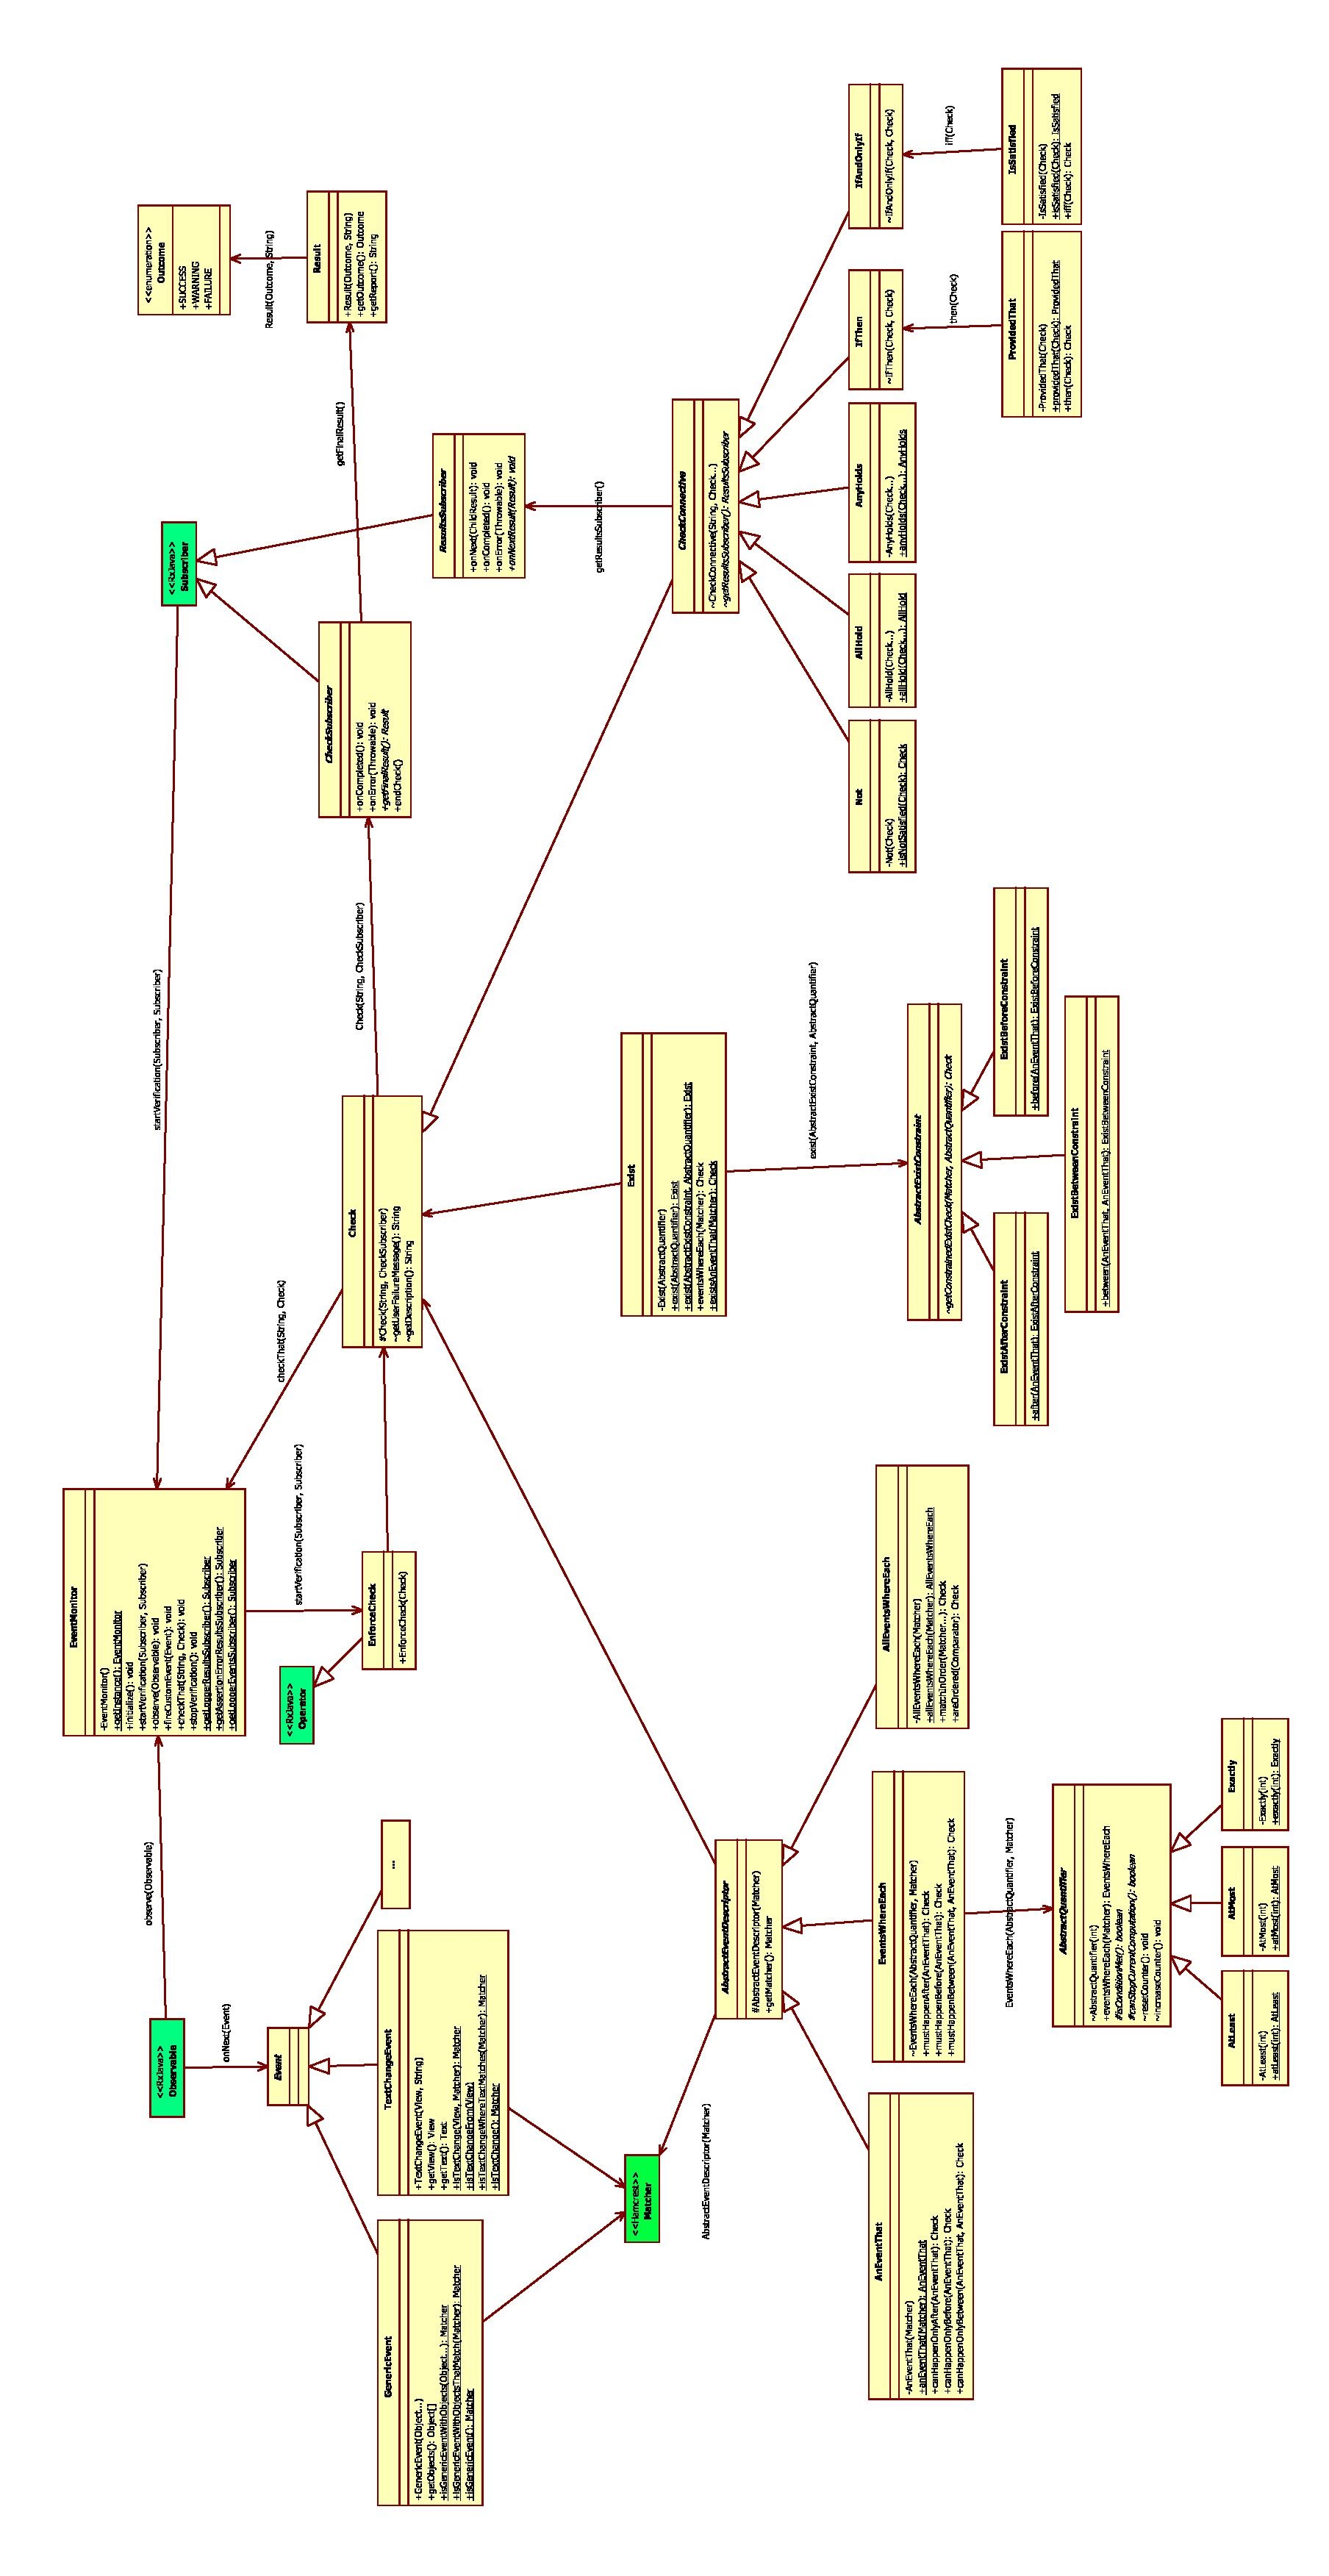
\includegraphics[height=\textheight]{Images/Event/UML/Implementation.jpg}
  \caption[Event-Based Testing Implementation UML]{UML Diagram for the Event-Based Testing Implementation}
  \label{fig:event_uml_implementation}
\end{figure}
The structure of the implementation of event-based testing is similar to what has been designed in section \ref{event_design}.\bigskip \\
A class diagram of the system is proposed in figure \ref{fig:event_uml_implementation}. Before starting the detailed explanation, note that many classes, like the descriptors, have a private constructor and a static method to create an instance. Similarly to the standard way of building assertions in JUnit, this is just syntactic sugar that allows to statically import the methods and to avoid writing the \texttt{new} keyword. These methods, and as a consequence their classes, are worded as close as possible to the English language: for example, the descriptor for single events is not called \textit{SingleEvent} but \texttt{AnEventThat} in order to build readable statements like:
\begin{lstlisting}
anEventThat(isTextChange())
	.mustHappenAfter(anEventThat(isButtonClick())
\end{lstlisting}

\subsection{Event Monitor}
The \texttt{EventMonitor} is a singleton class that is set up via the \texttt{initialize()} method. Once this is done, the developer can add Observables via \texttt{observe(Observable)} to build the event stream and checks via \texttt{checkThat(String, Check)}. This latter method also takes a String message as parameter representing an error shown if the check fails, similarly to standard assertions.\medskip \\
At this point a call to \texttt{startVerification(Subscriber<Event>, Subscriber<Result>)} is performed to start the validation process on the defined stream: the two Rx Subscribers are used by the developer to receive all the events of the stream in order and all the results of the checks respectively. The class provides some static methods to get simple pre-generated Subscribers for this purpose, e.g. passing \texttt{EventMonitor.getAssertionErrorResultsSubscriber()} as the second parameter the app crashes (or makes the test case fail) if a failure result is found.\medskip \\
When the developer calls \texttt{stopVerification()} the stream is interrupted and all the remaining check results are generated.\medskip \\
Finally, the class also provides the utility method \texttt{fireCustomEvent(Event)} that allows to directly generate an \texttt{Event} without creating an \texttt{Observable}.\medskip \\
Note that the \texttt{EventMonitor} observes the events on the thread specified by each Observable (usually the main thread) and runs the checks in a separate thread to avoid possible slowdowns of the UI thread.\medskip \\
The \texttt{EventMonitor} can be used as:
\begin{itemize}
	\item Runtime monitor during the manual debugging phase of the application development: just like the standard assertions placed in production code, the developer can use the monitor for example inside an activity to log all events and the results of the checks.
	\item Testing mechanism: the developer can start the monitor at the beginning of a test and add some specific checks, then execute the actions allowed by the chosen testing framework and finally stop the monitor at the end. The monitor works as a standard assertion mechanism, making the test fail in case a consistency check is not successful. Note that this mechanism, since it's not framework-specific, can be used for any type of test, from unit to UI, and with any library. A code example of the EventMonitor used as a testing mechanism can be found in listing \ref{lst_event_test}.
\end{itemize}

\subsection{Event Generators}
As introduced, the event generators are implemented as \texttt{Observable} objects provided by RxJava, an example of which can be found in listing \ref{lst_event_custom_observable}. Each Observable added to the \texttt{EventMonitor} builds the event stream: in particular, all the Observables are combined using the RxJava Operator \texttt{merge()}, which transforms a set of Observables into a single one that emits all the events in their respective order.\medskip \\
The events generated by these Observables are subclasses of \texttt{Event}, of which just two have been reported in the diagram since there could be hundreds of them. An \texttt{Event} class may also provide one or more static methods to create matchers, as is shown for example in listing \ref{lst_event_custom_event}.

\subsection{Checks}
A \texttt{Check} implements is logic using a \texttt{CheckSubscriber}, a subclass of the RxJava \texttt{Subscriber}. This component receives all the events of the stream via \texttt{onNext(Event)} and performs some internal computation, possibly short-circuiting the validation calling \texttt{endCheck()}. The callback \texttt{getFinalResult()} is called to return the unique \texttt{Result} of the check. An example of check implementation can be found in listing \ref{lst_event_check}.\medskip \\
The \texttt{EventMonitor} applies a check on the event stream by calling the Operator \texttt{EnforceCheck} on it, which is in charge of transforming a stream of \texttt{Event} objects into a stream containing a single \texttt{Result}.\medskip \\
Connectives between checks are implementations of \texttt{CheckConnective}, which is in turn a subclass of \texttt{Check}. Each of them implements a \texttt{ResultsSubscriber} that, analogously to a \texttt{CheckSubscriber}, receives the results of its terms, performs some computation and then produces a single \texttt{Result} as output. \texttt{Not}, \texttt{AllHold} and \texttt{AnyHolds} (implementations of the logic \textit{negation}, \textit{and} and \textit{or} respectively) provide static methods as constructors (e.g. \texttt{allHold(check1, check2, check3)}), while \texttt{IfThen} and \texttt{IfAndOnlyIf} (implementations of \textit{single} and \textit{double implication}) are built starting from the \texttt{ProvidedThat} and \texttt{IsSatisfied} classes respectively (e.g. \texttt{providedThat(check1).then(check2)}), to make the calls more human-readable.

\subsection{Descriptors}
The descriptors are subclasses of \texttt{AbstractEventDescriptor}. \texttt{AnEventThat} (single event) and \texttt{AllEventsWhereEach} (all the events in the whole stream) provide static constructors, while \texttt{EventsWhereEach} descriptors (sets of events) do not provide one because they are built starting from a quantifier, e.g. \texttt{exactly(10).eventsWhereEach(...)}.\medskip \\
The \texttt{Exist} class provides the means to express the existential quantifiers, i.e. \texttt{existsAnEventThat(...)} and \texttt{exist(...).eventsWhereEach(...)}. The latter type uses quantifiers and constraints to define the cardinality of the set in the first case and the possible validity interval in the second.\medskip \\
Existential constraints are subclasses of \texttt{AbstractExistConstraint}. They simply implement an abstract method to define the constraint logic and provide a static method to be used in the existential check expressions.\medskip \\
Quantifiers are subclasses of \texttt{AbstractQuantifier}. Each of them uses an internal counter and overrides several methods like \texttt{isConditionMet()} and \texttt{canStopCurrentComputation()} to implement its logic. All of them have a private constructor and a static method like the descriptors.\medskip \\
The matchers that describe the type of events identified by each descriptor are implemented using the external library JavaHamcrest~\cite{Hamcrest}, a well known way to describe objects. The library provides several matchers on the most common objects (like Strings, e.g. \texttt{isEmptyString()}, \texttt{startsWith(String)}, etc.), some connectives to compose matchers (e.g. \texttt{allOf(Matcher...)}) and the means to implement custom matchers, which have been used to define matchers for the events.

\fxnote*{New}{\section{Evaluation}}

\subsection{Applicability}
The event-based testing library is most suitable for applications that are characterized by a high number of different operations that can possibly run concurrently. This usually means applications that heavily employ the network (i.e. that query the web in background), the device sensors (e.g. receive GPS events to update a map) and/or, in general, that perform several sub-routines in parallel thanks to Services and threads.\medskip \\
However, the library may be applicable also to more "sequential" applications, especially for the event counting and ordering capabilities, e.g. the developer might be interested in easily quantifying the number of click events during a particular execution.\medskip \\
Event-based testing is especially useful for applications that already use the ReactiveX library in production code since the Observables to generate the events are already built.\medskip \\
The library can be applied both as a testing support tool, expressing conditions during test cases built in Espresso, Robolectric or any other framework, or as a debugging tool directly in production code in the early stages of development, to observe how the event stream is built.

\subsection{Effectiveness}
To discuss the effectiveness of the event monitor tool we can focus on three aspects:
\begin{itemize}
	\item Event Stream Composition: it may be noted that, thanks to the available listeners and RxAndroid extensions, many events can be easily observed in an Android application, like user interaction on most View components, sensor data, broadcasts, etc. However, there are many events that cannot easily be observed, mainly because Android does not provide any listener on which to build the ReactiveX Observable (e.g. no listener is available to see when a View element becomes visible or hidden) or because it only allows to manage a single listener (e.g. only one focus change listener is allowed per View component and, if the developer uses one inside the production code of the application, RxJava cannot use another to build the Observable). This of course can limit the event stream composition and, as a consequence, the possible checks that can be expressed on it.
	\item Assertions Language Expressiveness: the proposed assertion language allows to express temporal constraints (events can happen only after/before/between other events), causality (events must happen after/before/between other events), existence, ordering and quantification among events, as well as correlating check results via logic connectives. This expressiveness allows to express the majority of temporal operators, but may be extended in future work to support more complex assertions, for example like the possibility of correlating the matched events between several checks.
	\item Results Handling: the result of each consistency check contains an outcome (success, failure or warning) and a report message to understand its meaning. For example, the result of the check asserting that a text change event can only happen after a fragment started can contain the report \textit{The event $\left\{\mbox{Text change "MyText" from TextView1}\right\}$ was found before an event that is a fragment lifecycle event "onStart"}, which clearly shows what event made the check fail. Moreover, the event monitor offers the possibility of printing the whole event stream as it was registered during the execution, allowing the developer to analyze it to find possible causes of a bug.
\end{itemize}

\subsection{Usability}
The generation effort to build the event stream depends on the specific application and on what the developer wants to achieve. If the events that need to be observed are covered by one of the RxAndroid extensions listed in section \ref{android_observables} the generation of the Observables is straightforward. However, if the developer needs to observe Android events not covered by any extension or events specific to the application under test, it may be required to build custom Observables. Usually, creating a custom Observable is not a complex task because of the RxJava library support, but in some cases it may require some effort.\medskip \\
With regard to the consistency checks, the effort required for their specification is mostly due to the "logic" approach. Developers are used to express sequential conditions on the current state of the component under test, so they might find difficult to adapt to the temporal assertions language, that requires to specify conditions that must hold throughout the entire test execution. Nevertheless, care has been taken to offer a language as close as possible to the English language, to allow the developers to easily write and understand the meaning of a check at first glance.\medskip \\
Finally, it may be noted that the library is not framework-specific. This means that it can be easily employed in any testing framework, like Espresso, Robolectric or the built-in instrumented unit testing, provided that it is able to observe all the required events in the application

\subsection{Performance}
The performance overhead introduced by the event-based testing library is, in general, negligible. For example, in the case of the test suite described in section  \ref{event_eval_real}, executing the same Espresso test with and without the Event Monitor (with 2 tests, 7 checks each and more than 130 observed events) a performance degradation of less than 3\% was registered (an average of 40 seconds with the monitor active against an average of 39 seconds without any event-related condition).\medskip \\
This is due to the fact that the RxJava library provides a very lightweight and scalable event handling system and to the implementation of the checks as Subscribers that perform very simple operations at each event of the stream. Moreover, the check logic is implemented in a separate thread from the main UI thread of the Android application, in order not to decrease the app responsiveness.\medskip \\
It can also be noted that is some situations it may be required to edit the production code to insert custom event firing, when a listener is not available. This, however, does not create any issue when the application is run outside the event-based test case. If the \texttt{EventMonitor} component is not initialized, any call to add Observables, checks or fire custom events is ignored and so the performance is not degraded. Moreover, it is possible to completely remove these calls in "release" builds (e.g. the application is made available on the Play Store) with tools like ProGuard~\cite{ProGuard}.

\subsection{Extensibility}
The library can be extended by the developer to adapt it to the specific needs of the application under test. In particular, a developer can implement:
\begin{itemize}
	\item Custom Events and Matchers: it is enough to extend the \texttt{Event} class, providing any parameter and Hamcrest matcher required.
	\item Custom Observables: to inject custom events in the stream the developer just needs to create a ReactiveX Observable.
	\item Custom Subscribers: the library provides simple Subscribers for both the event stream and the check results, but the developer can build custom implementations by simply implementing a ReactiveX Subscriber. This allows to manage the event monitor results in any way, from logging to saving them in a database or file.
	\item Custom Checks: it is also possible to build customized checks and check connectives, by implementing a ReactiveX Subscriber that, receiving all the events of the stream, keeps a state and returns one final result.
\end{itemize}

\subsection{Comparison with Testing Frameworks}
Comparing temporal assertions with the standard Android testing frameworks like Espresso, Robolectric and the instrumented unit tests, the event-based testing approach can be seen both as an extension and as an alternative.\medskip \\
It is an extension because the event monitor is a tool that needs to be executed during a standard test case, since it is necessary to define the tested components and the actions (e.g. clicks) to be performed.\medskip \\
It is, however, also an alternative to the standard assertions that can be used during these tests. If we consider the example of assessing that an AsyncTask starts only after the user clicks on a button, it can be easily expressed with a temporal check but it is very complex to specify it with standard assertions. It would require for example to continuously poll the AsyncTask variable before the click action to check if the task is running (or to manually setup a test listener invoked when the task starts) and, using boolean variables, assert that one is always false before the other becomes true.

\subsection{Comparison with Race Detection Tools}
Comparing the proposed solution with race detectors like EventRacer and DEvA, it is first important to stress the fact that the approach is different. The mentioned tools try to detect possible race conditions, either dynamically or statically, without requiring the developer to write any test case. In the event-based testing library, instead, the focus is on manually generated test cases that allow to verify conditions on the event stream. For this reason, event-based testing is proposed as a complementary tool, and not as an alternative.\medskip \\
From the point of view of race conditions, it can be noticed that the two approaches mostly focus on different types races.
\begin{itemize}
	\item EventRacer and DEvA focus their attention mainly on data races, i.e. they detect when two or more callbacks that use the same variable may be in conflict. If we consider the example (reported in listing~\ref{lst_event_race_detectors}) of a button click callback where a Service is invoked and a connection callback where the Service is initialized, a race might be detected by the tools. In this example, it does not necessarily mean that the click callback cannot happen before the connection one, but just that the developer should handle that situation, e.g. by checking if the Service variable is null in the click callback before using it and, if so, just show a message to the user.
	\item The event-based testing approach, instead, focuses on races between events that cannot be verified in any possible execution, i.e. specifying that a given event can happen only after/before/between other given events. An example (reported in listing~\ref{lst_event_race_eventbased}) of this can be the situation where the application logic imposes that text change events of an email contents can happen only before the user clicks on the "Send" button.
\end{itemize}
Given this distinction, we can have races that:
\begin{itemize}
	\item Can only be recognized by race detection tools: the example of the click-connection race cannot be expressed with temporal assertions since the two callbacks may happen in any order.
	\item Can only be tested by the event-based approach: the example of the text changes before the click cannot be recognized by the race detectors since there is no variable in common between the click and the text change callbacks.
	\item Can be both recognized by race detectors and tested with the event-based approach: an example (reported in listing~\ref{lst_event_race_both}) of this is the event of placing a marker on a map when this has not been initialized yet. These two events generated by the application without user interaction must never be in the wrong order, otherwise the application might crash or result in the marker not being placed on the map. This condition can be expressed with a temporal assertion and, since we have a common variable (the map object), it may be recognized by race detectors.
\end{itemize}\medskip
Moreover, with the proposed library the developer is able to focus on events in general, and not only on race conditions like the aforementioned tools. This means that there is the possibility of looking at the event stream generated by an execution from a broader perspective, being also able to express conditions on existence, ordering and quantification of events.

\subsection{Real-World Application}\label{event_eval_real}
As a real-world example of event-based testing application, the WordPress for Android app was chosen. The idea is to define some temporal assertions on the latest version at the time of writing~\cite{WordPress2016-07-15}, to discuss the expressiveness of the language, the generation effort and the types of events that can be observed.\medskip \\
In particular, this evaluation focuses on the \texttt{EditPostActivity}, which allows the users to write and publish a post on their blog. The Activity contains an instance of \texttt{EditorFragment}, which manages the fields for writing the post content, and uses the \texttt{PostUploadService} to publish the post and the \texttt{MediaUploadService} to add an image or video to the content.

\subsubsection{Structure}
The test suite of the aforementioned example is defined in Espresso and can be visualized in listing~\ref{lst_event_test}. The Activity under test is defined by a \texttt{IntentsTestRule}, an object similar to \texttt{ActivityTestRule} but specific for Intent mocking (used to simulate the image selection). The test case uses the callbacks provided by the \texttt{IntentsTestRule} to manage the Event Monitor:
\begin{itemize}
	\item During \texttt{beforeActivityLaunched()}, called before each test starts, the monitor is initialized.
	\item During \texttt{afterActivityLaunched()}, called just after the tested Activity is started, Observables and checks can be added. Since the method is called for each test, the Observables and checks added here are valid for all the defined test cases.
	\item During \texttt{afterActivityFinished()}, called after each test ends, the Event Monitor verification is terminated.
\end{itemize}
After the definition of the \texttt{IntentsTestRule} object, the developer can specify one or more test cases that use the Event Monitor. First of all, in each of them further Observables and checks, which are specific for that test, can be added, and then the validation process is started. At this point, the developer defines the standard UI actions of an Espresso test, to drive the application execution.\bigskip \\
Given this structure, the Event Monitor executes in the background of a normal Espresso test, observing all the events generated by the UI actions and validating the defined checks, similarly to the standard assertions mechanism.

\subsubsection{Events}
The test for the \texttt{EditPostActivity} observes both imported and custom events, including:
\begin{itemize}
	\item Text change events on title and content fields of the post.
	\item Toast (quick and short messages displayed to the user as feedback) display.
	\item Media upload start, progress and completion.
	\item Post upload start.
	\item Click on menu options, like the "Publish" button.
	\item Lifecycle events of the Activity and Fragment under test.
	\item HTML mode toggle event (while writing the post the user can switch between visual and HTML modes).
\end{itemize}\medskip
The imported events include for example the text change events of title and content of the post, observed thanks to the RxBinding module. Since they are easily observable by just calling a single method, these events do not require any particular coding effort by the developer.\medskip \\
Most of the events, however, are specific for the WordPress application, for example the HTML toggle event and the media upload progress event. As such, these events need to be created by the developers, together with the proper Hamcrest matchers, similarly to what can be seen in listing~\ref{lst_event_custom_event}. The generation effort of the event classes is very low, to define the custom events for the WordPress application less than a couple of minutes per class were required.\medskip \\
Once the custom events are defined, they either need to be fired manually (i.e. modifying the production code of the application) using the \texttt{EventMonitor\#fireCustomEvent(Event)} method (in case of lack of valid listeners, like in the case of the HTML toggle event) or an Observable must be generated. An example of the latter case is the media upload progress events Observable, defined in listing~\ref{lst_event_custom_observable}. The generation effort of the Observables highly depends on the specific case (i.e. available listeners): in this case, to define the Observable for media upload progress events took approximately five minutes.

\subsubsection{Checks}
The defined checks, valid for all the tests, enforce the following conditions:
\begin{itemize}
	\item The HTML mode cannot be activated while a media item is uploading, for an application logic constraint.
	\item The post title and content cannot change after the publication procedure has started.
	\item Clicking on the "Publish" button must always be followed either by a Toast display (e.g. an error occurred) or by the publication procedure start, i.e. there cannot be situations where the button is unresponsive.
	\item If the Editor Fragment is detached from the host Activity (e.g. the application is closed) while a media upload is in progress, the upload must be interrupted.
	\item Before the publication procedure starts, all media uploads must complete.
	\item The media upload progress values must be sent in order, i.e. there cannot be situations where the service sends incoherent percentages of uploaded content.
\end{itemize}
The test case \texttt{testPublishError()} also adds a specific check that states that the click on the "Publish" button must generate an error saying that the post is empty.\medskip \\
Once the checks are defined, the developer can stress-test the application (e.g. try several sequences of actions, drive the application lifecycle, etc.) to see if the defined temporal assertions hold in all possible situations.\medskip \\
Regarding the generation effort, once the condition to be verified has been identified, the generation of the check specification took approximately five minutes each.

\subsubsection{Check Results}
Since the objective of this evaluation was not to stress-test the application for bug detection but just to show how the library can be applied in a real-word context, only a couple of Espresso tests were specified to drive the application execution and, as a consequence, all the defined check results were successful.\medskip \\
For example, the outcomes printed by the tool during the \texttt{testUploadImage()} test were:
\begin{itemize}
	\item \texttt{[SUCCESS] No event that is any HTML toggle event happens between a pair of events where the first is media upload progress and the second is any media upload outcome (success/failure/cancel)\\
REPORT: The condition was never met between any of the 1 pairs}
	\item \texttt{[SUCCESS] IF (Exists an event that is post upload start) THEN (Every event that is post change happens before an event that is post upload start)\\
REPORT: Every event that is post change was found before $\left\{\text{Post upload start}\right\}$}
	\item \texttt{[SUCCESS] Every event that is click on menu option <2131821737> is followed by at least 1 events where each (is post upload start or is any toast display)\\
REPORT: Check verified for each of the 1 events where each is click on menu option <2131821737>}
	\item \texttt{[SUCCESS] IF (exactly 1 events where each is a fragment lifecycle event \char`\"onDetach\char`\"~are between at least one pair of events where the first is media upload progress and the second is any media upload outcome (success/failure/cancel)) THEN (Every event that is a fragment lifecycle event \char`\"onDetach\char`\"~is followed by at least 1 events where each is media upload cancel)\\
REPORT: The pre-condition didn't hold: The condition was never met between any of the 1 pairs}
	\item \texttt{[SUCCESS] NOT TRUE THAT (at least 1 events where each is post upload start are between at least one pair of events where the first is media upload progress and the second (is any media upload outcome (success/failure/cancel) or is media upload progress))\\
REPORT: The condition was never met between any of the 131 pairs}
	\item \texttt{[SUCCESS] All events where each is media upload progress are in the order defined by the comparator: org.wordpress.android.ui.posts.EditPostActivityTest$1$1@a746538\\
REPORT: All 131 events were in order}
\end{itemize}


%..............................................................................%
%................................. CONCLUSION .................................%
%..............................................................................%

\newpage
\part{Conclusions and Future Work}\label{part_conclusion}

\fxnote*{New}{
\section{Conclusions}
This thesis presented a possible \fix{possible? perhaps comprehensive, covering different development stages and tasks} testing approach that focuses on the events generated during the execution of an Android application. It analyzed first a subset of events, lifecycle transitions, and then focused on a more generic concept of events.\medskip \\
Section \ref{section_lifecycle_static} proposed a static analysis approach for lifecycle testing, focusing on the management of selected components according to the host Activity/Fragment lifecycle. This approach is mainly useful in the early stages of development to warn the developer of possible criticalities, concerning performance or correctness.\medskip \\
In section \ref{section_lifecycle_dynamic}, instead, it is reported the description of a dynamic approach for lifecycle testing. The idea is to provide a more complete support for lifecycle testing, hiding to the developers the complexity of driving the transitions and so allowing them to just focus on actions and assertions defined in the test case. The relevance of thoroughly testing an Activity or a Fragment with regard to its lifecycle is an important step to ensure confidence of correctness of the component, since lifecycle handling can often generate many issues.\medskip \\
Part \ref{part_events} proposed an event-based testing library. The idea is to first build an event stream, observing different Android events defined by the developer, and then to express consistency checks on it, using a temporal assertions language. This allows to check for a specific type of race conditions and to assess existence, ordering and quantification of the events generated during the application execution.\medskip \\
Finally, it is interesting to note that the three approaches proposed by the thesis can all be employed at the same time. For example, the developers may use the static lifecycle checks to easily spot problems while coding the application, then define test cases that exploit both temporal assertions and lifecycle tests to verify the consistency in the event stream during critical lifecycle transitions.

\section{Future Work}
Possible future extensions on the proposed work include:
\begin{itemize}
	\item For static lifecycle testing:
	\begin{itemize}
		\item Provide more static checks implementations, such as camera, location updates, etc.
		\item Extend the static analysis scope by providing more complex checks. It may be possible not only to focus on release, double instantiation and best practices but also, for example, to build a complete graph of usages per each component with regard to the host Activity/Fragment lifecycle and to analyze it for possible critical aspects.
		\item Provide a mechanism to automatically fix, whenever possible, the detected problems.
	\end{itemize}
	\item For dynamic lifecycle testing:
	\begin{itemize}
		\item Provide a better testing interface: for example it may be possible to avoid the subclassing and the implementation of the abstract callback methods by providing annotations that automatically generate the required tests. This would allow to define more tests of the same type (e.g. two rotation tests in the same test suite) and to avoid methods that return null if the developer is not interested in some test cases.
		\item Provide testing not only for Activities but also for Fragments. This would require to create a new testing mechanism (e.g. Fragment Test Rule), since it is not provided by Android.
		\item Automatically generate appropriate lifecycle test cases for selected Activities or Fragments, with automated assertion placement.
	\end{itemize}
	\item For event-based testing:
	\begin{itemize}
		\item Provide a better support for building the event stream, i.e. allow in some way to observe events that do not have an Android listener or to easily observe other events without the need to edit the production code (e.g. it may be possible to observe any callback invocation with aspect-oriented programming).
		\item Increase the assertion language expressiveness, adding more checks and allowing to specify dependencies among sub-checks in check connectives.
		\item Provide a better check results handling: for example, it may be possible to write a more complete report on the event monitor outcome, with cleaner interface (e.g. generating an HTML file) and more information to allow the developer to understand the problem more easily and to reproduce the behavior in other tests.
		\item Evaluate the possibility of reordering the events in the stream (e.g. by automatically generating delays in the invocation of callbacks) to better test the consistency among events.
		\item Provide automated assertion placement support, allowing the developer to start from relevant pre-generated temporal assertions.
	\end{itemize}
\end{itemize}
}


%..............................................................................%
%................................. APPENDICES .................................%
%..............................................................................%

\newpage
\begin{appendices}
\addcontentsline{toc}{part}{Appendices}

\fxnote*{New}{\section{Code Listings}}
%\setcounter{lstlisting}{0}
\lstset{
  numbers=left,
  frame=single
}

\lstinputlisting[label={lst_lifecycle_wp},caption={Example of lifecycle test. In particular, it is the test case defined for the \texttt{MyProfileActivity} in the WordPress app that checks if, after a rotation, the inserted name is kept.}]{Listings/LifecycleDynamic/ExampleWP.java}

\lstinputlisting[label={lst_event_race_first},caption={Example of race condition: if the user rotates the device while the AsyncTask is running, the application crashes with an \texttt{IllegalStateException}.}]{Listings/Event/RaceExampleFirst.java}

\lstinputlisting[label={lst_event_test},caption={Example of Espresso test that uses the event-based testing library, defined for the \texttt{EditPostActivity} of the WordPress app.}]{Listings/Event/CompleteTestImplementation.java}

\lstinputlisting[label={lst_event_custom_event},caption={An example of custom event implementation for event-based testing: the HTML toggle event in the WordPress app. It can have any parameter (in this case just a boolean), provide several static methods to build Hamcrest matchers and define the \texttt{toString} method, whose output is used by the EventMonitor.}]{Listings/Event/EventImplementation.java}

\lstinputlisting[label={lst_event_custom_observable},caption={An example of custom Observable for event-based testing: generates the media-related events in the WordPress application. \texttt{EventBusObservable} just provides a static method to easily get the Observable, \texttt{EventBusSubsriber} is an abstract class created for reuse and \texttt{MediaUploadOnSubscribe} is the actual implementation of the Rx Observable that fires the events.}]{Listings/Event/ObservableImplementation.java}

\lstinputlisting[label={lst_event_check},caption={An example of check implementation for event-based testing: the "can happen only between" of \texttt{AnEventThat}. The subscriber is implemented as a finite state machine that handles the events in order, changing state and/or short-circuiting the check if we have a match.}]{Listings/Event/CheckImplementation.java}

\lstinputlisting[label={lst_event_race_detectors},caption={Race condition that can be recognized by detectors like EventRacer or DEvA but cannot be expressed with a temporal assertion.}]{Listings/Event/RaceExampleDetectorsOnly.java}

\lstinputlisting[label={lst_event_race_eventbased},caption={Race condition that can be expressed with a temporal assertion but cannot be recognized by detectors like EventRacer or DEvA.}]{Listings/Event/RaceExampleEventBasedOnly.java}

\lstinputlisting[label={lst_event_race_both},caption={Race condition that can be both recognized by detectors like EventRacer or DEvA and expressed with a temporal assertion.}]{Listings/Event/RaceExampleBoth.java}

\end{appendices}

\newpage
\listoffigures
\addcontentsline{toc}{part}{List of Figures}

%..............................................................................%
%.................................. REFERENCES ................................%
%..............................................................................%

\newpage

\fix{You can merge all these bib files in one and reference just that one file}

\bibliographystyle{unsrt}
\bibliography{Bib/DEvA,Bib/CAFA,Bib/EventRacer,Bib/JUnit,Bib/Lint,Bib/Mockito,Bib/Oracles,Bib/ReactiveLocation,Bib/ReactiveNetwork,Bib/ReactiveSensors,Bib/Retrofit,Bib/Robolectric,Bib/RxAndroid,Bib/RxBinding,Bib/RxBroadcast,Bib/RxFileObserver,Bib/RxGoogleMaps,Bib/RxJava,Bib/RxLifecycle,Bib/RxPermissions,Bib/RxPreferences,Bib/RxWear,Bib/StorIO,Bib/THOR,Bib/CountingLogic,Bib/Hamcrest,Bib/Stats,Bib/InTheClear,Bib/TrackBuddy,Bib/WordPressApp,Bib/WordPressCMS,Bib/WordPress2015-12-06,Bib/WordPress2016-07-15,Bib/ERVA,Bib/SoftwareTestingAndAnalysis,Bib/Espresso,Bib/UIAutomator,Bib/monkeyrunner,Bib/UIExerciserMonkey,Bib/ProGuard,Bib/StaticLifecycleChecks,Bib/DynamicLifecycleTesting,Bib/EventBasedTesting,Bib/ReactiveX} 
\addcontentsline{toc}{part}{References}

\end{document}


